\section{GeoFit Corrections}
\label{sec:app_geofitcorr}
Reconstructed muons in CMS can have non-zero d0 values. If the d0 value is a result of reconstructing a slightly wrong track for the muon, this can cause a shift in the \pt of the muon. This \pt shift causes an increase in overall dimuon mass resolution due to a smearing of the dimuon mass peak reconstructed from muons with non-zero d0 values. Fig.~\ref{fig:2D_Z_mass_vs_d0} shows 2D plots derived from Z+jets MC samples which show the pulls in fitted values for dimuon mass peaks versus d0 values of the $\mu^+$ and $\mu^-$. There is a clear trend in the fitted dimuon mass peak values such that the peak value increases along $\text{d0}_{\mu^+}-\text{d0}_{\mu^-}$ direction. As can be seen in Fig.~\ref{fig:2D_Z_mass_vs_d0} the effect is consistent in both data and MC and since the muon \pt values used in these plots are after the \textit{Rochester Corrections} it is clear that this effect is not fixed by them. Therefore there is a need for a different correction to fix the dependence of muon \pt values on the muon d0 values. 

\begin{figure}[h!]
    \centering
    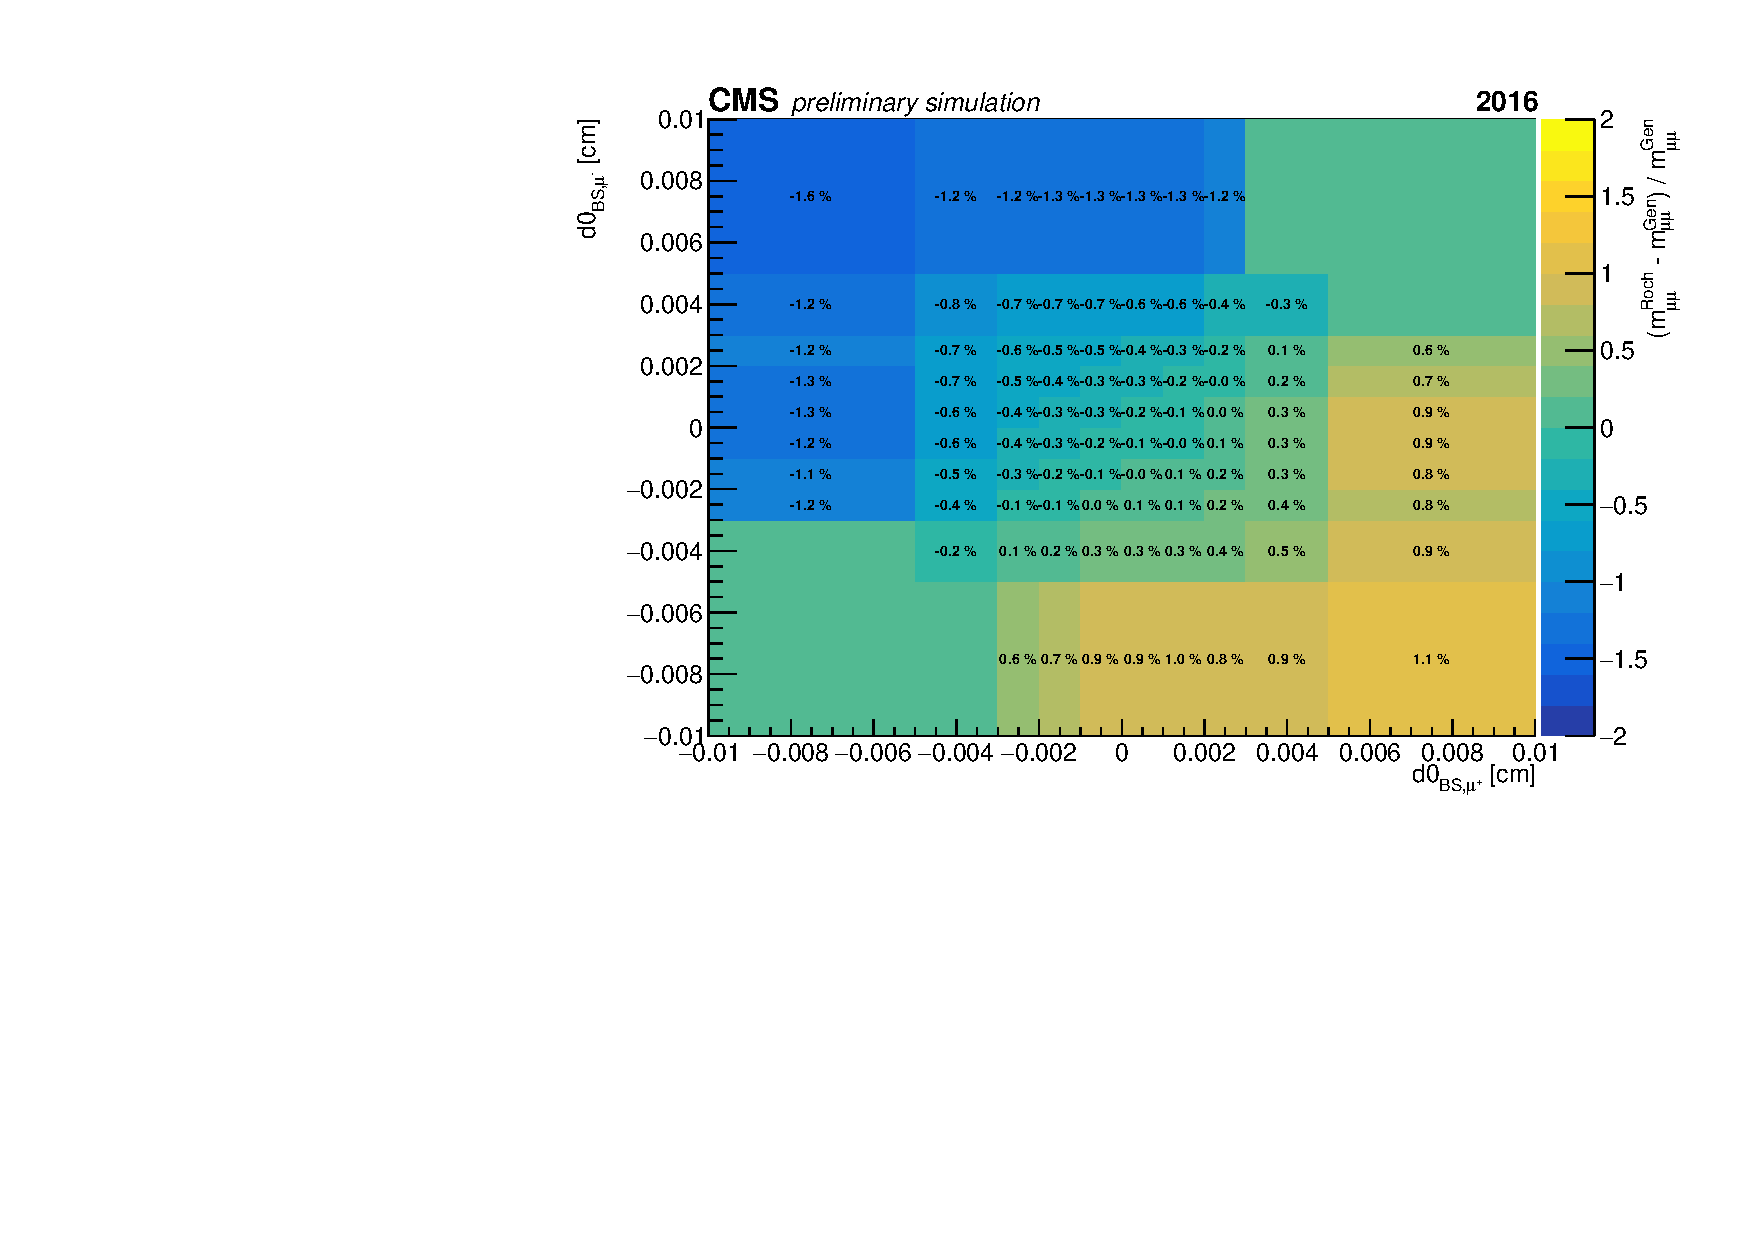
\includegraphics[width=0.49\textwidth]{images_geofit/2D_Z_mass_vs_d0_pulls.pdf}
    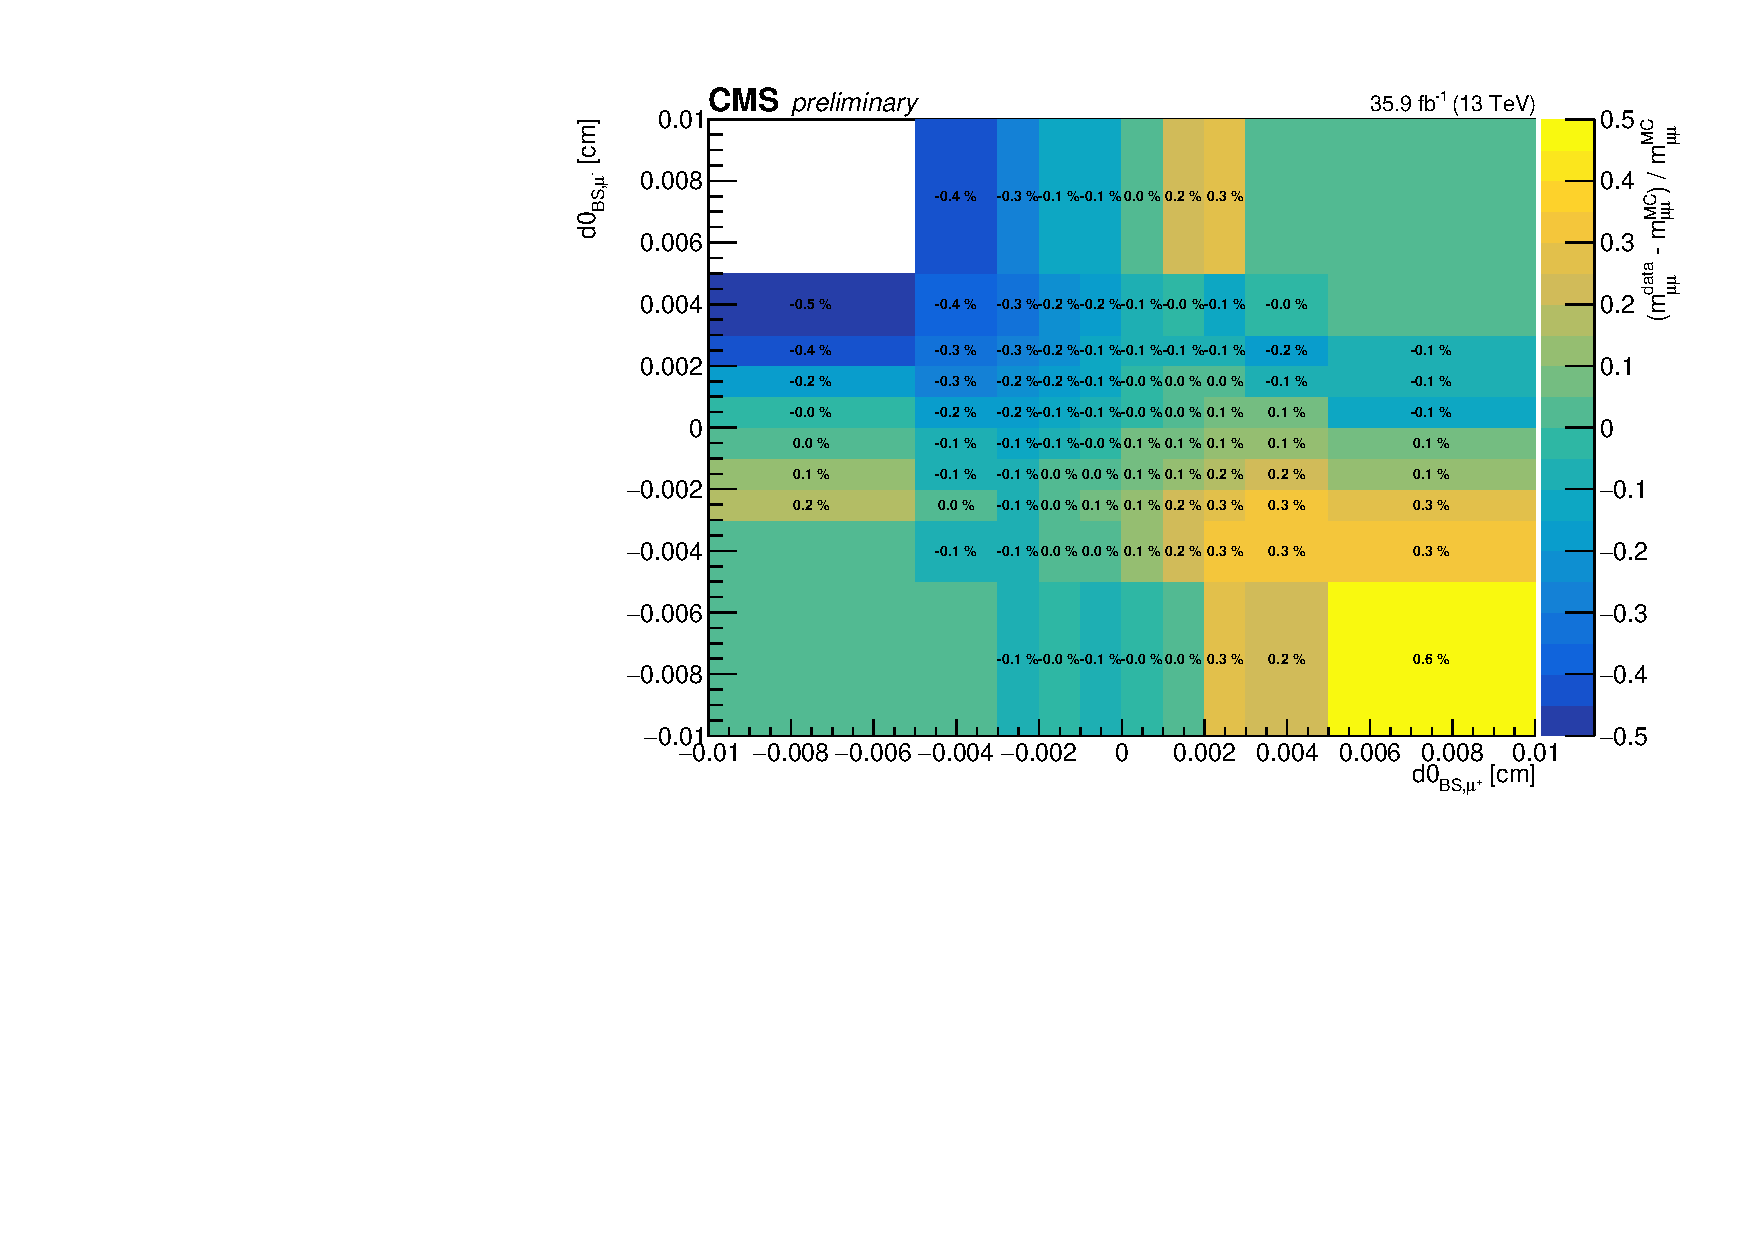
\includegraphics[width=0.49\textwidth]{images_geofit/2D_Z_mass_vs_d0_data_MC.pdf}
    \caption{2D maps showing pulls on dimuon mass around Z boson mass peak, comparing reconstructed mass and generator level mass (left) and data and MC (right) binned in $\text{d0}_{\mu^+}$ and $\text{d0}_{\mu^-}$ for Z+jets MC samples from 2016.}
    \label{fig:2D_Z_mass_vs_d0}
\end{figure}

A simple geometric inspection shows that in tracks that are bent by the magnetic fields, d0 values are related to the radius of curvature of the tracks as follows:

\begin{equation}
  d0 \sim \frac{\Delta R}{R^2}
\label{eqn:d0_R}
\end{equation} 

Since in homogeneous magnetic fields $\pt \sim R$, we can write the above equation as:

\begin{equation}
  d0 \sim \frac{\Delta \pt}{\pt^2} 
\label{eqn:d0_pt}
\end{equation}

Therefore the shift in \pt of the muons due to this effect can be corrected by finding the constant of proportionality in Eq.~\ref{eqn:d0_pt}. The correction derived using this procedure is named \textit{GeoFit Corrections} due to its geometric motivation. 

The constant of proportionality of \textit{GeoFit Corrections} may depend on other factors such as muon $\eta$, muon $\phi$, pileup, etc. Since the constant of proportionality between d0 and \pt depends on the magnetic field, we expect muon $\eta$ to have an effect on this effect. Furthermore, since muon charge affects the direction the muon bends in magnetic field we expect this effect to have reversed sign for $\mu^-$ compared to $\mu^+$. Therefore, in this study the value of d0 is always multiplied by muon charge to take this effect into account. The effects of other variables on \textit{GeoFit Corrections} are harder to guess, and in order to understand these effects all of these dependencies should be studied.

Firstly, the definition of d0 that is used in these corrections needs to be determined. In general, d0 values for muons are defined as the distance of closest approach of the muon track to the PV (\dzeroPV). It is calculated as $\text{d0} = -x_0\sin(\phi_0) + y_0 \cos(\phi_0)$ where $(x_0,y_0)$ are the coordinates of the point on the track closest to the PV, and $\phi_0$ is the azimuthal angle of the track at that point. However, since PV is determined by the tracks of physics objects in an event, in events with few high \pt tracks the PV position tends to be closer to these tracks. This results in calculated \dzeroPV values to be smaller than the true values. Another useful d0 parameter can be calculated by using the \textit{beam spot} (BS) instead of PV, and is denoted as \dzeroBS. Since BS is calculated over several events, it has a more averaged out position which is less biased towards high \pt tracks. Figures~\ref{fig:d0_data_MC_comparisons} show the distribution of \dzeroPV and \dzeroBS values of the leading muon for data and MC samples. As can be seen from these figures, \dzeroPV distributions have a sharper peak at the middle of the distribution which is stacked on top of a wider peak which is in line with our reasoning.

\begin{figure}[h!]
    \centering
    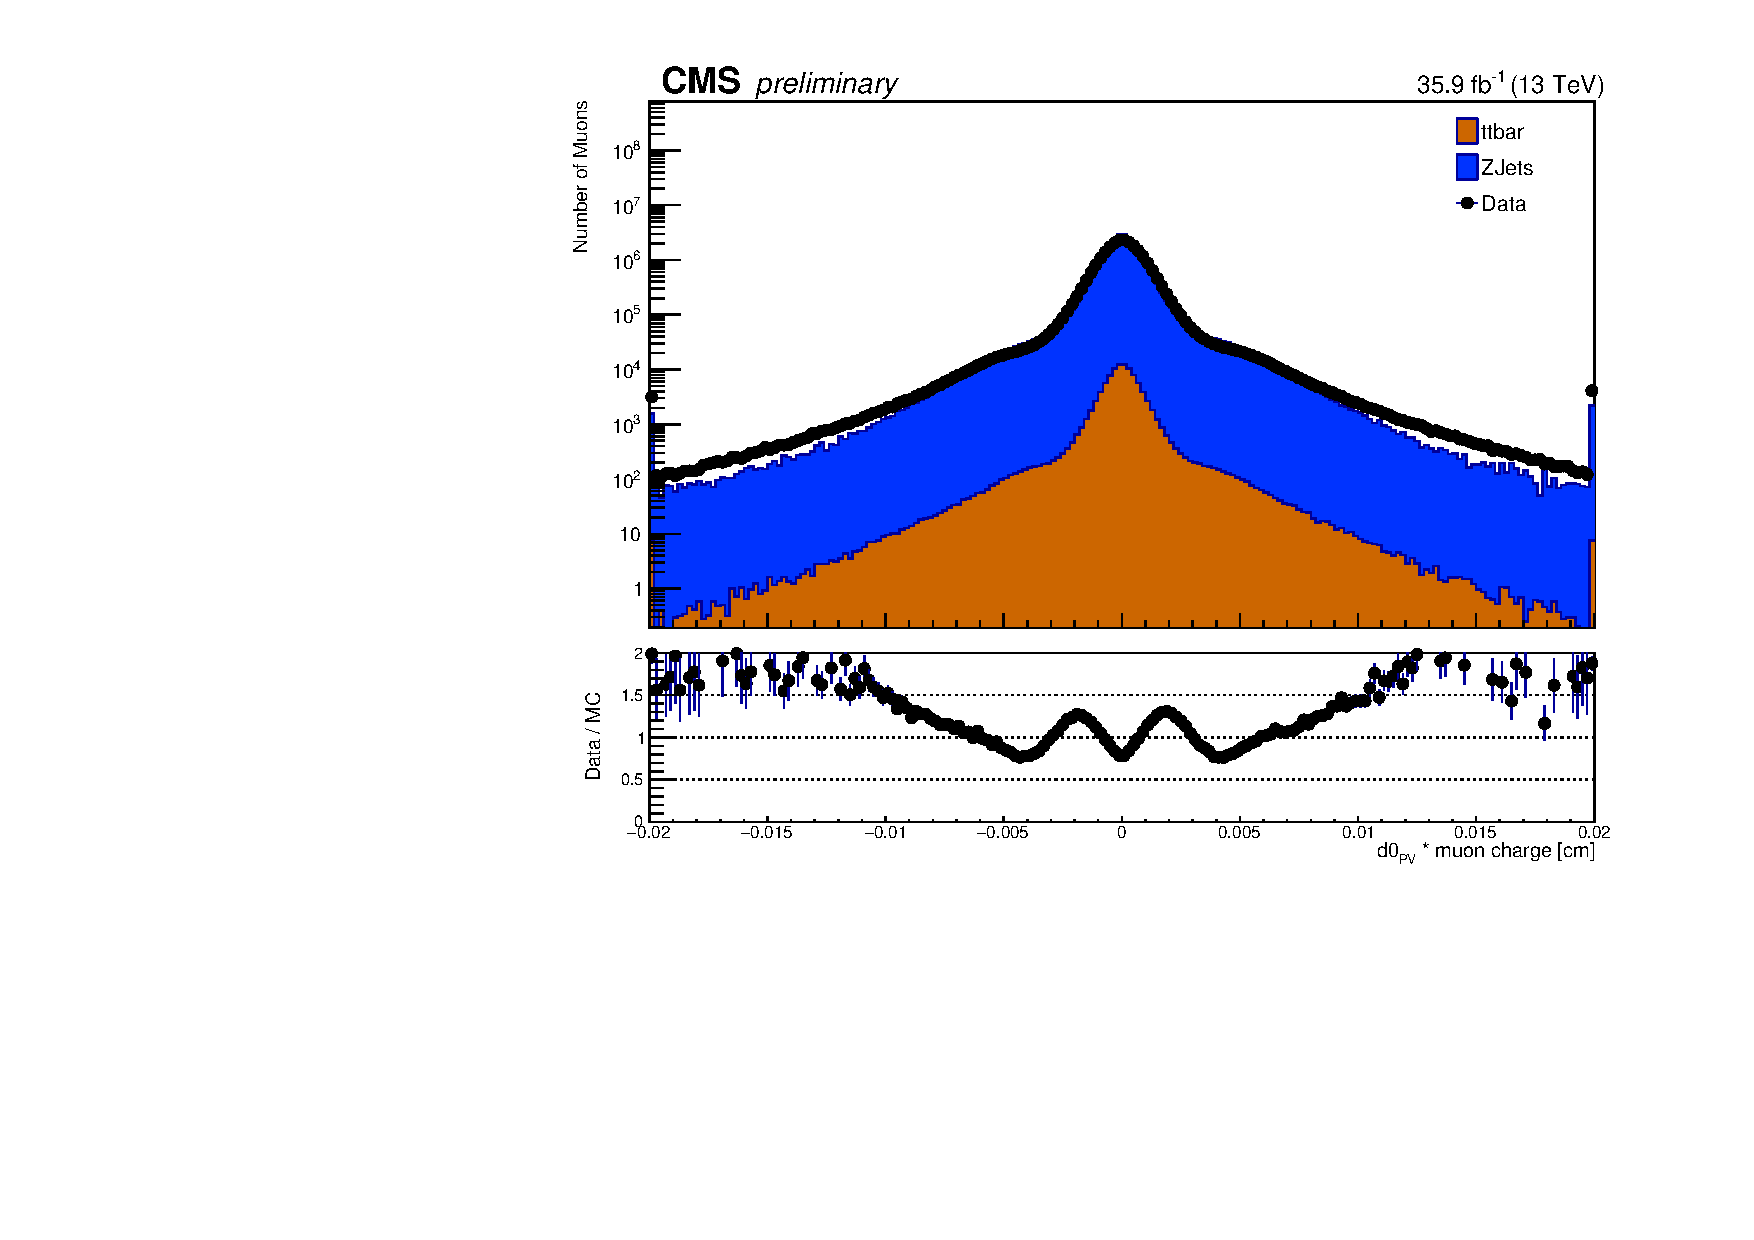
\includegraphics[width=0.49\textwidth]{images_geofit/d0_PV_data_MC_comp.pdf}
    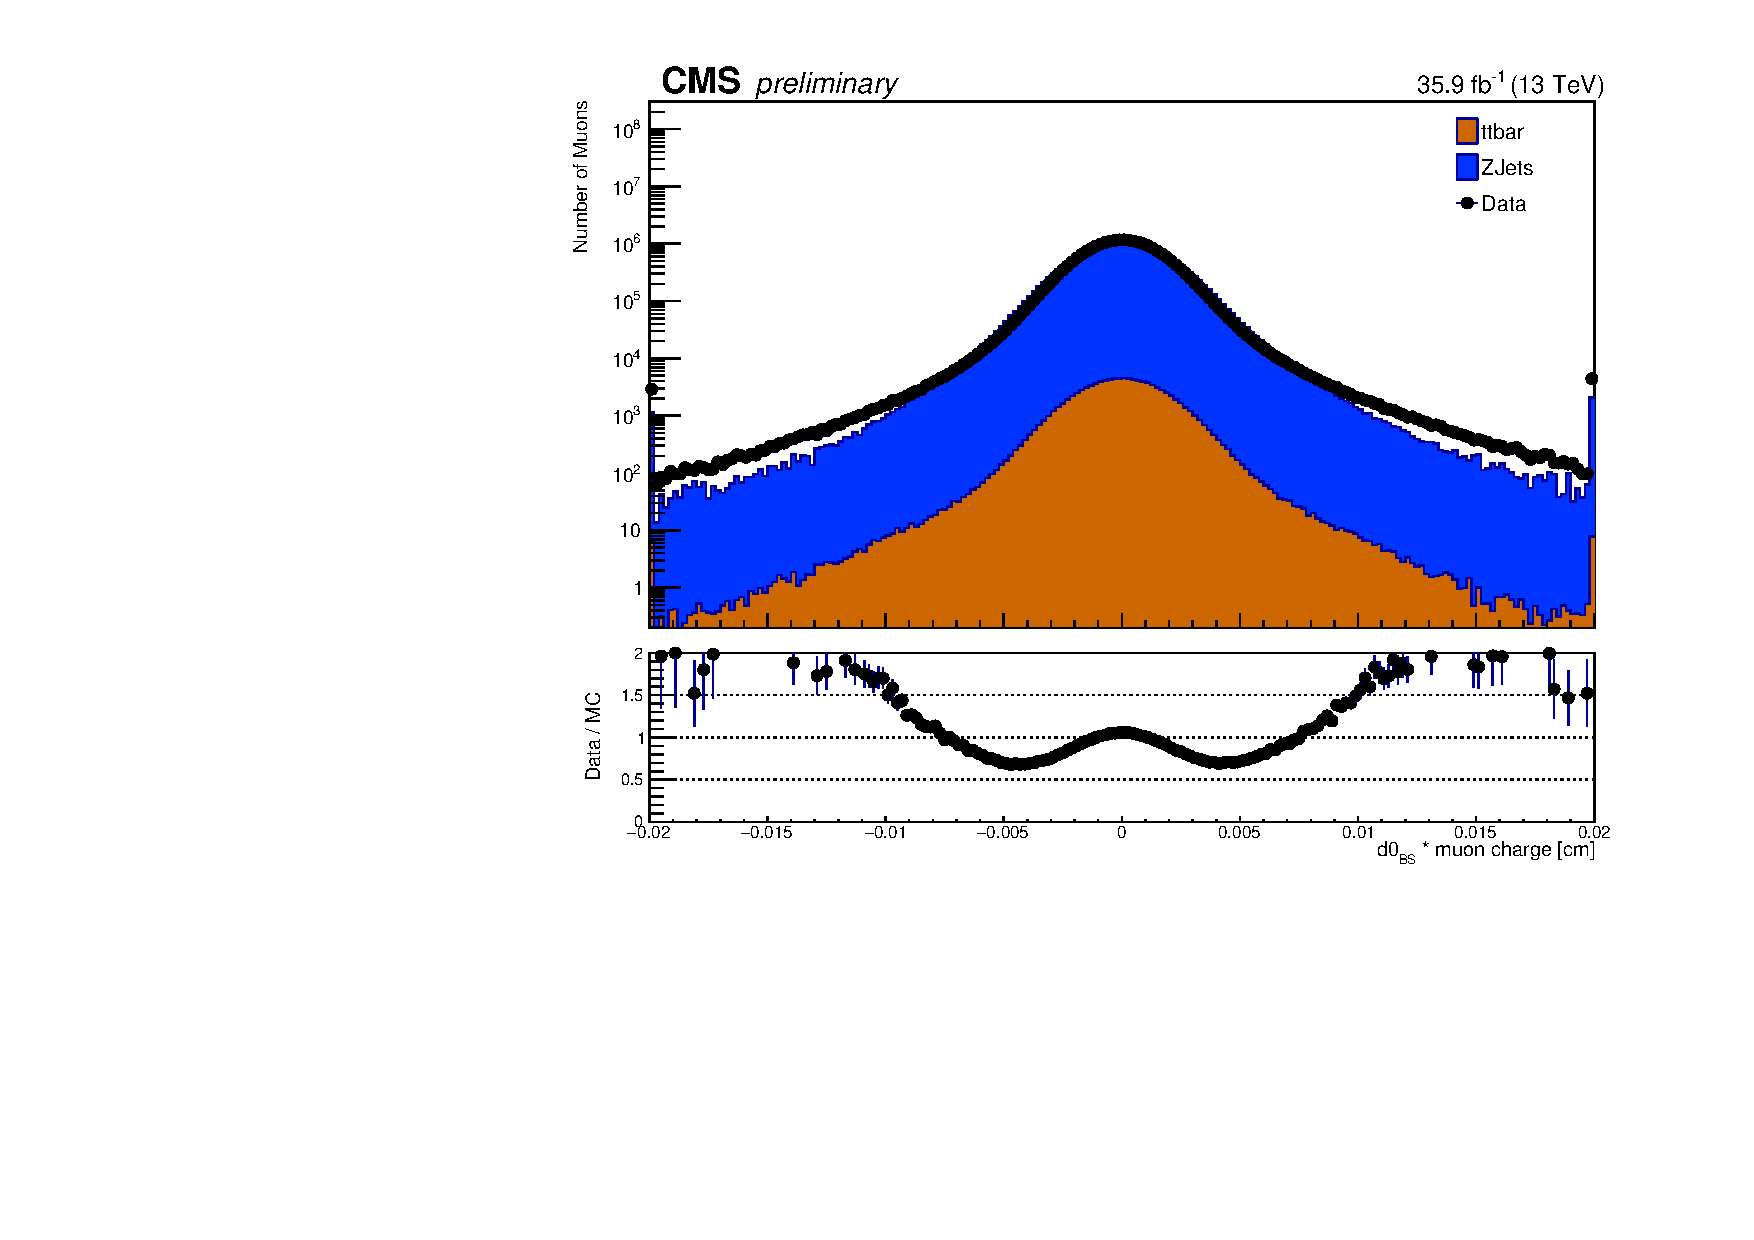
\includegraphics[width=0.49\textwidth]{images_geofit/d0_BS_data_MC_comp.pdf}
    \caption{Plots showing comparisons of \dzeroPV (left) and \dzeroBS (right) of leading muon between data and MC. \dzeroPV plot shows the narrow peak around zero, while \dzeroBS distribution does not have a similar feature.}
    \label{fig:d0_data_MC_comparisons}
\end{figure}

In order to inspect the effect of using \dzeroPV or \dzeroBS further, Figures~\ref{fig:2D_d0_dpTOverpT2_inclusive} contain 2D plots derived from Z+jets MC samples that display the number of muons in bins of \dptoverptsquare and \dzeroPV or \dptoverptsquare and \dzeroBS. From these plots we can see that the linear relationship between \dptoverptsquare and \dzeroBS is more pronounced compared to \dzeroPV. 

\begin{figure}[h!]
    \centering
    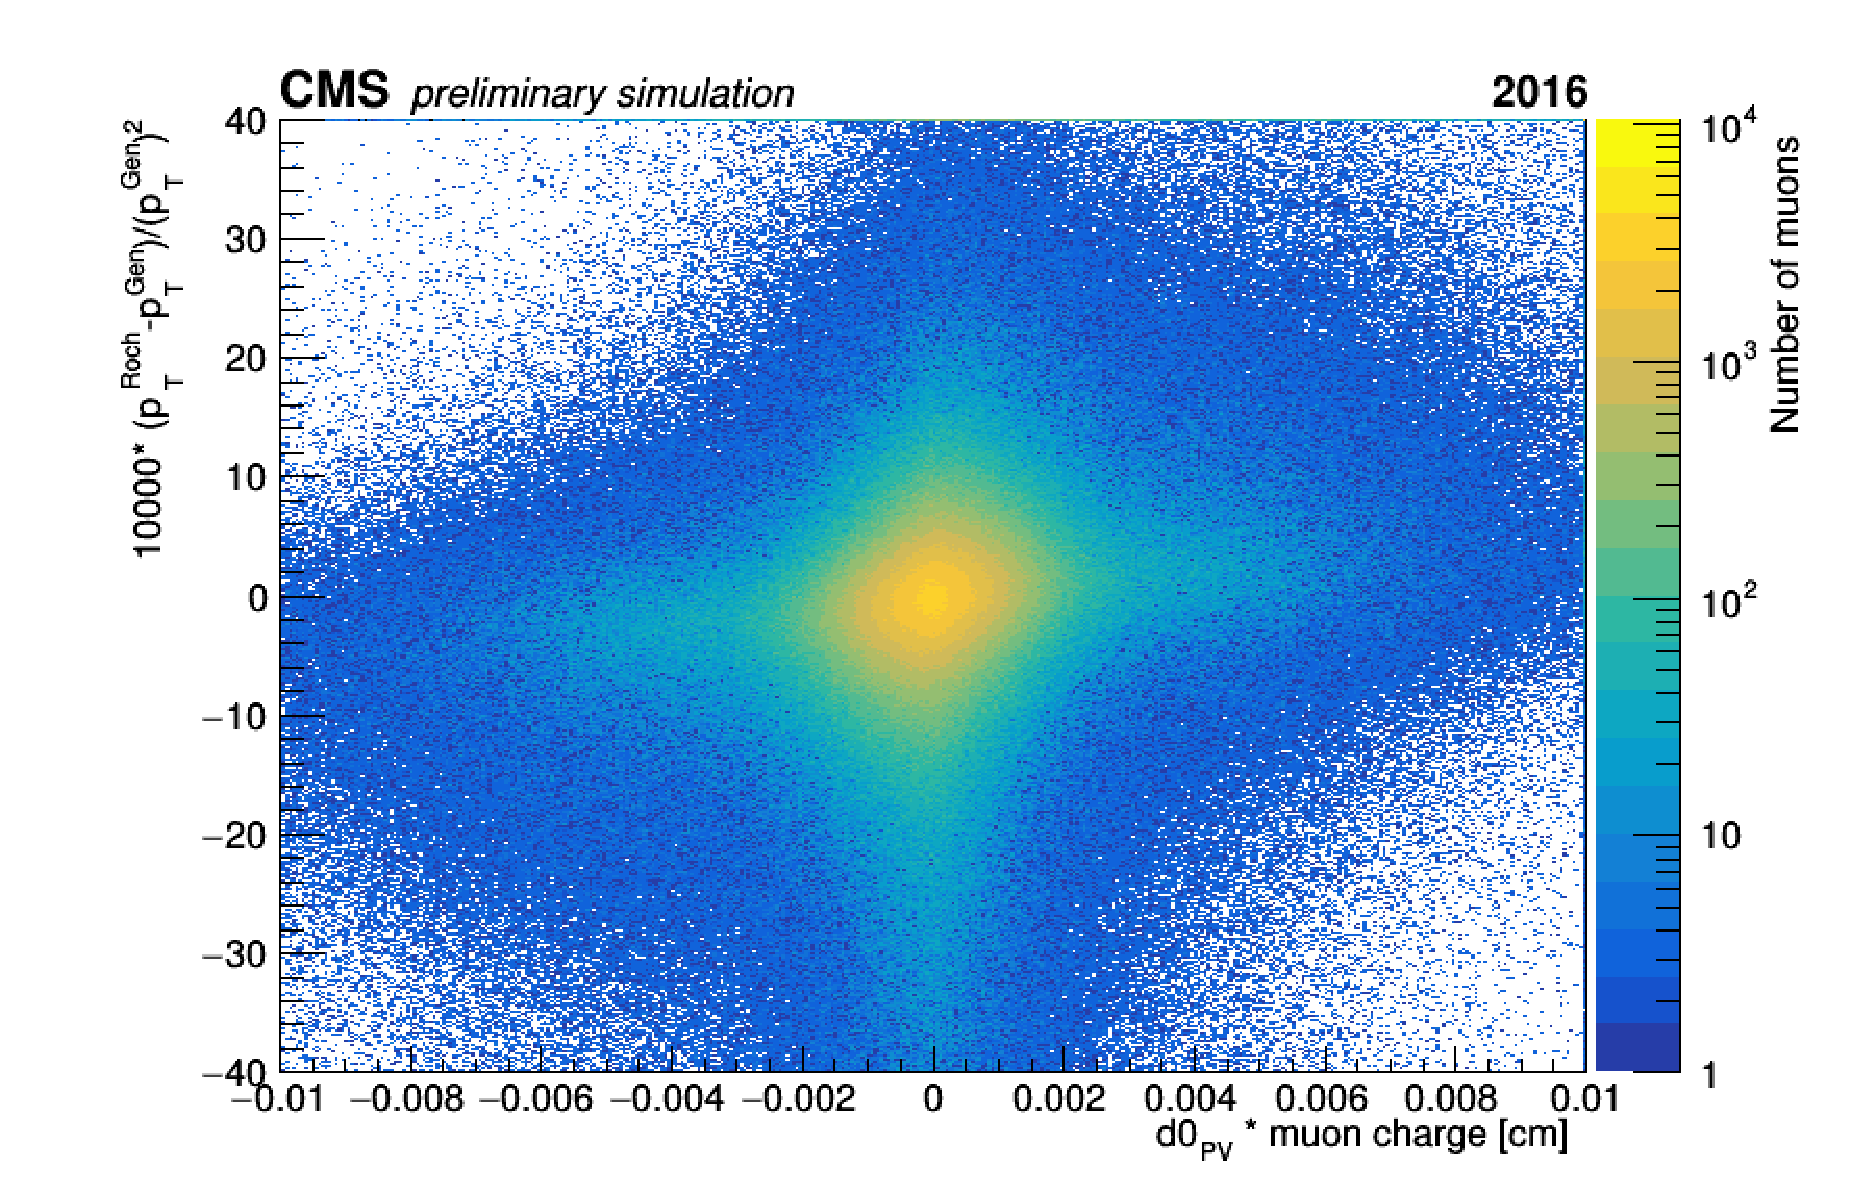
\includegraphics[width=0.49\textwidth]{images_geofit/2D_d0_PV_dpTOverpT2_lowRes.pdf}
    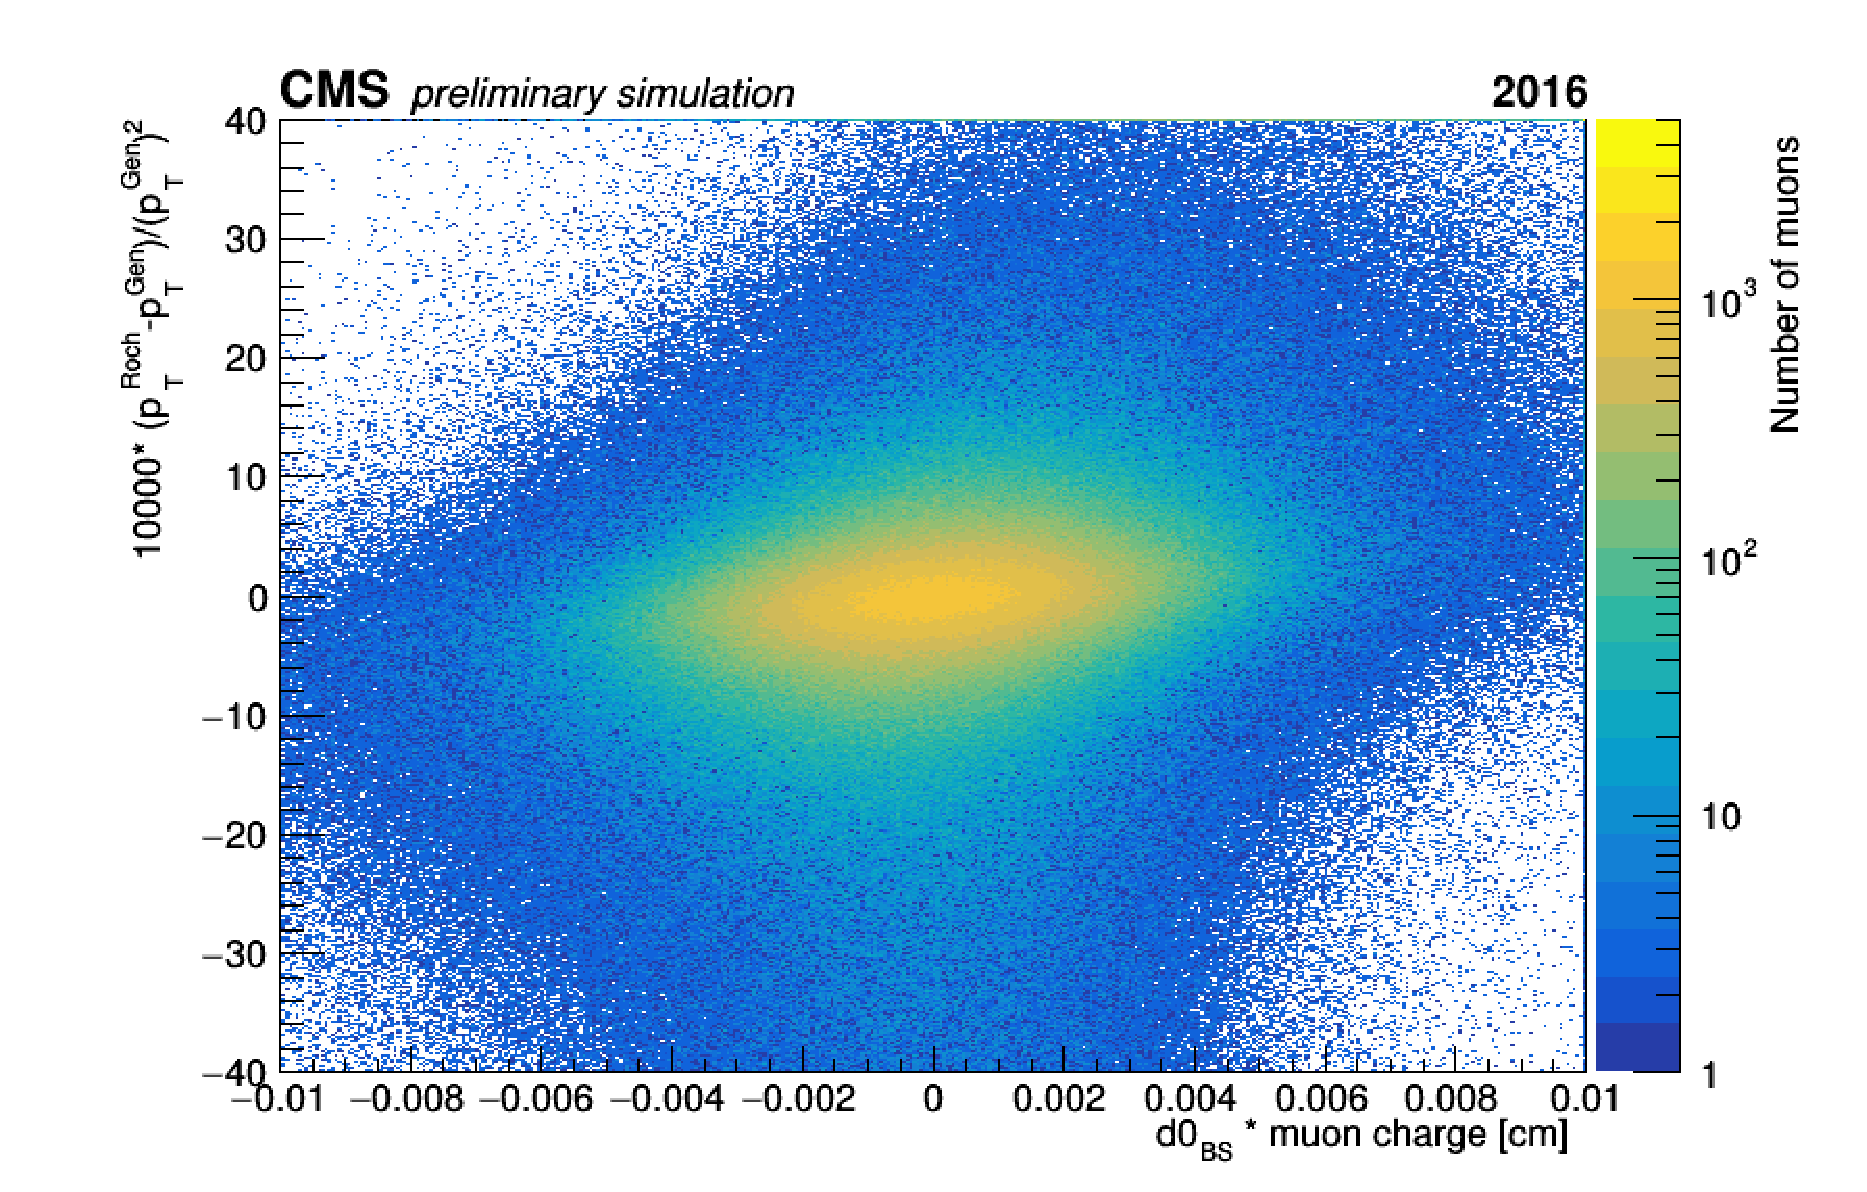
\includegraphics[width=0.49\textwidth]{images_geofit/2D_d0_BS_dpTOverpT2_lowRes.pdf}
    \caption{2D maps showing number of muons in bins of \dptoverptsquare and \dzeroPV (left) and \dptoverptsquare and \dzeroBS (right). The linear relationship is more pronounced in the right plot, whereas the left plot have a more concentrated and circular distribution near the center.}
    \label{fig:2D_d0_dpTOverpT2_inclusive}
\end{figure}

In order to extract the constant of proportionality, we take slices of \dzeroPV or \dzeroBS and find the peak and width of Gaussian-like \dptoverptsquare distributions in these slices. Figures~\ref{fig:d0_dpTOverpT2_inclusive} show data points which represents the positions of the peaks for each of the d0 slices with error bars representing the width of these distributions in each slice. As can be seen from these plots, the distributions with \dzeroBS show a clear linear dependence between \dptoverptsquare and \dzeroBS whereas the distributions with \dzeroPV show a non-linear dependence. Therefore \dzeroBS is a better handle to calculate the effect of non-zero muon d0 on muon \pt, and is chosen to be used throughout these corrections.

\begin{figure}[h!]
    \centering
    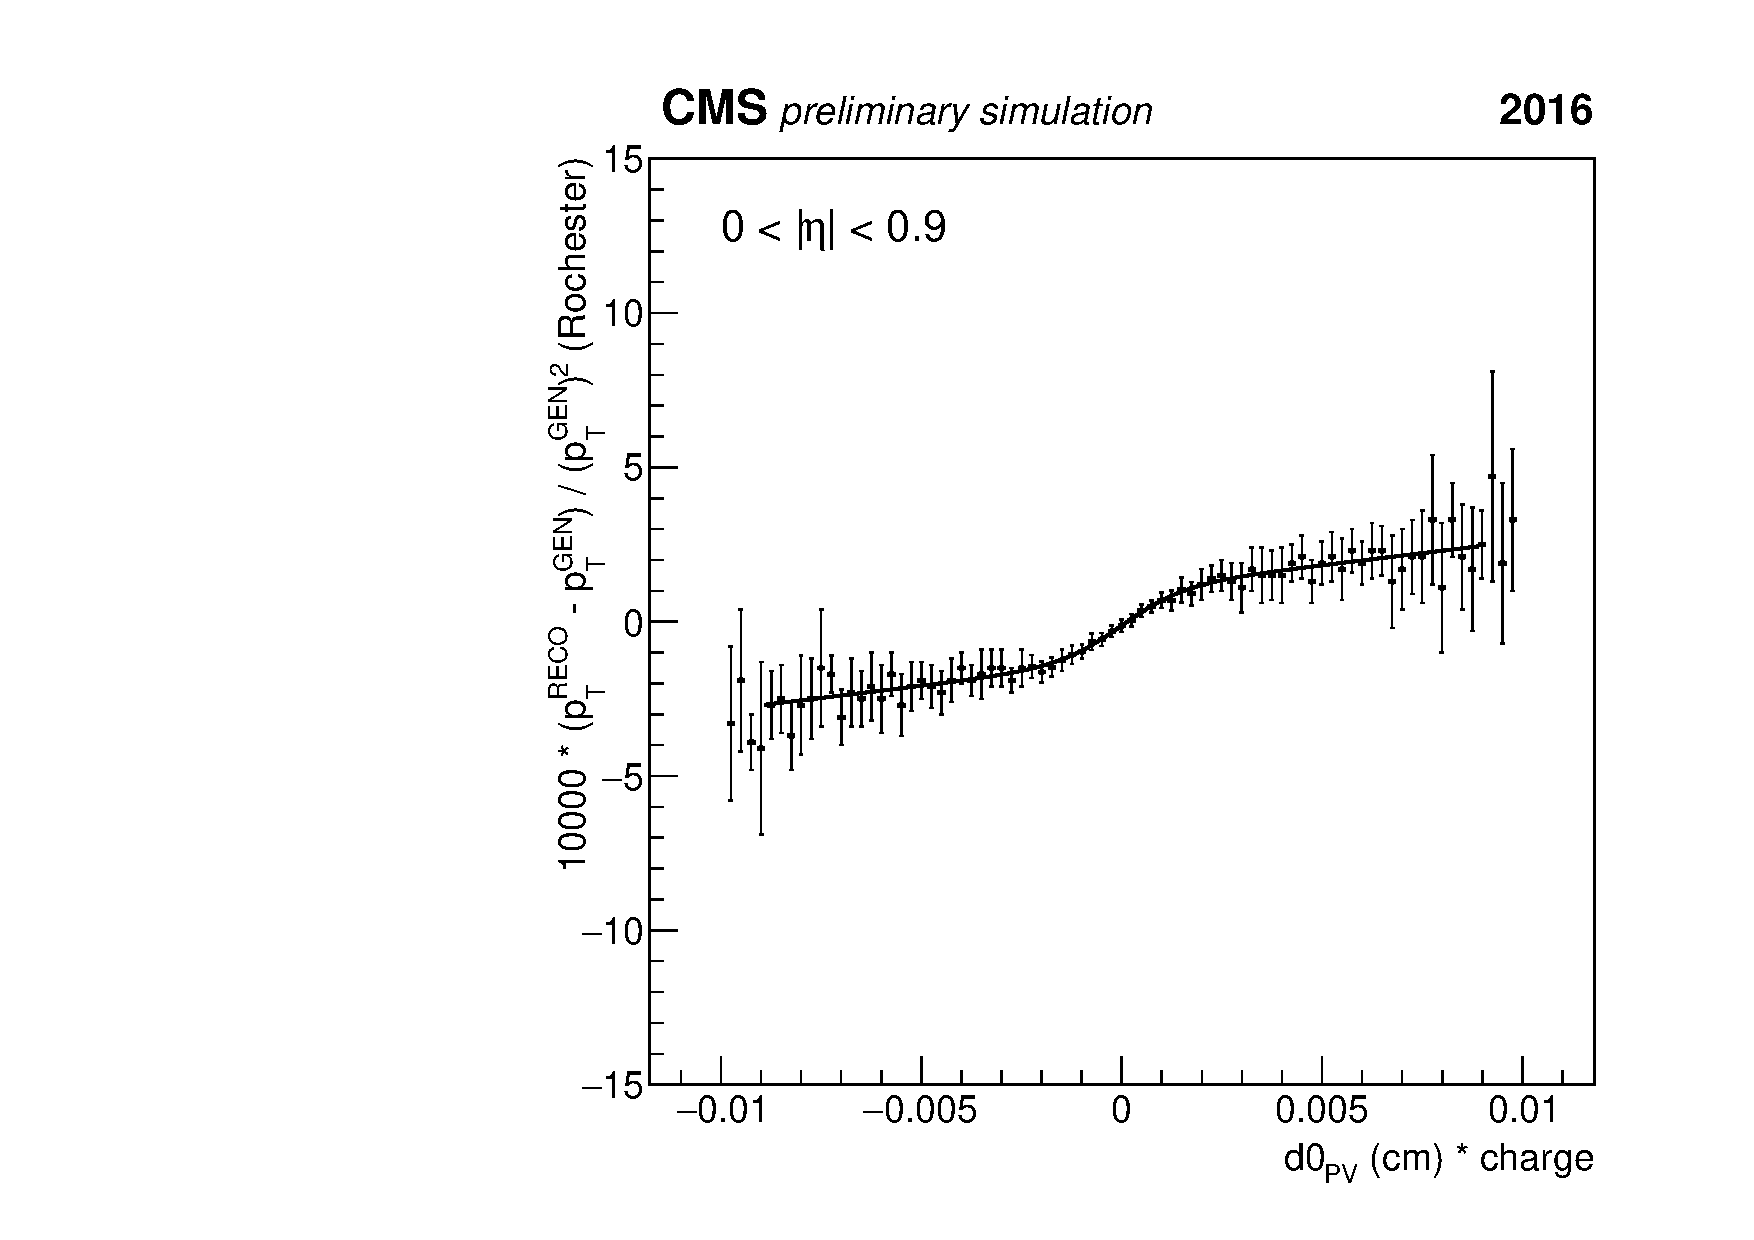
\includegraphics[width=0.49\textwidth]{images_geofit/d0_PV_dpTOverpT2_eta_0_0p9.pdf}
    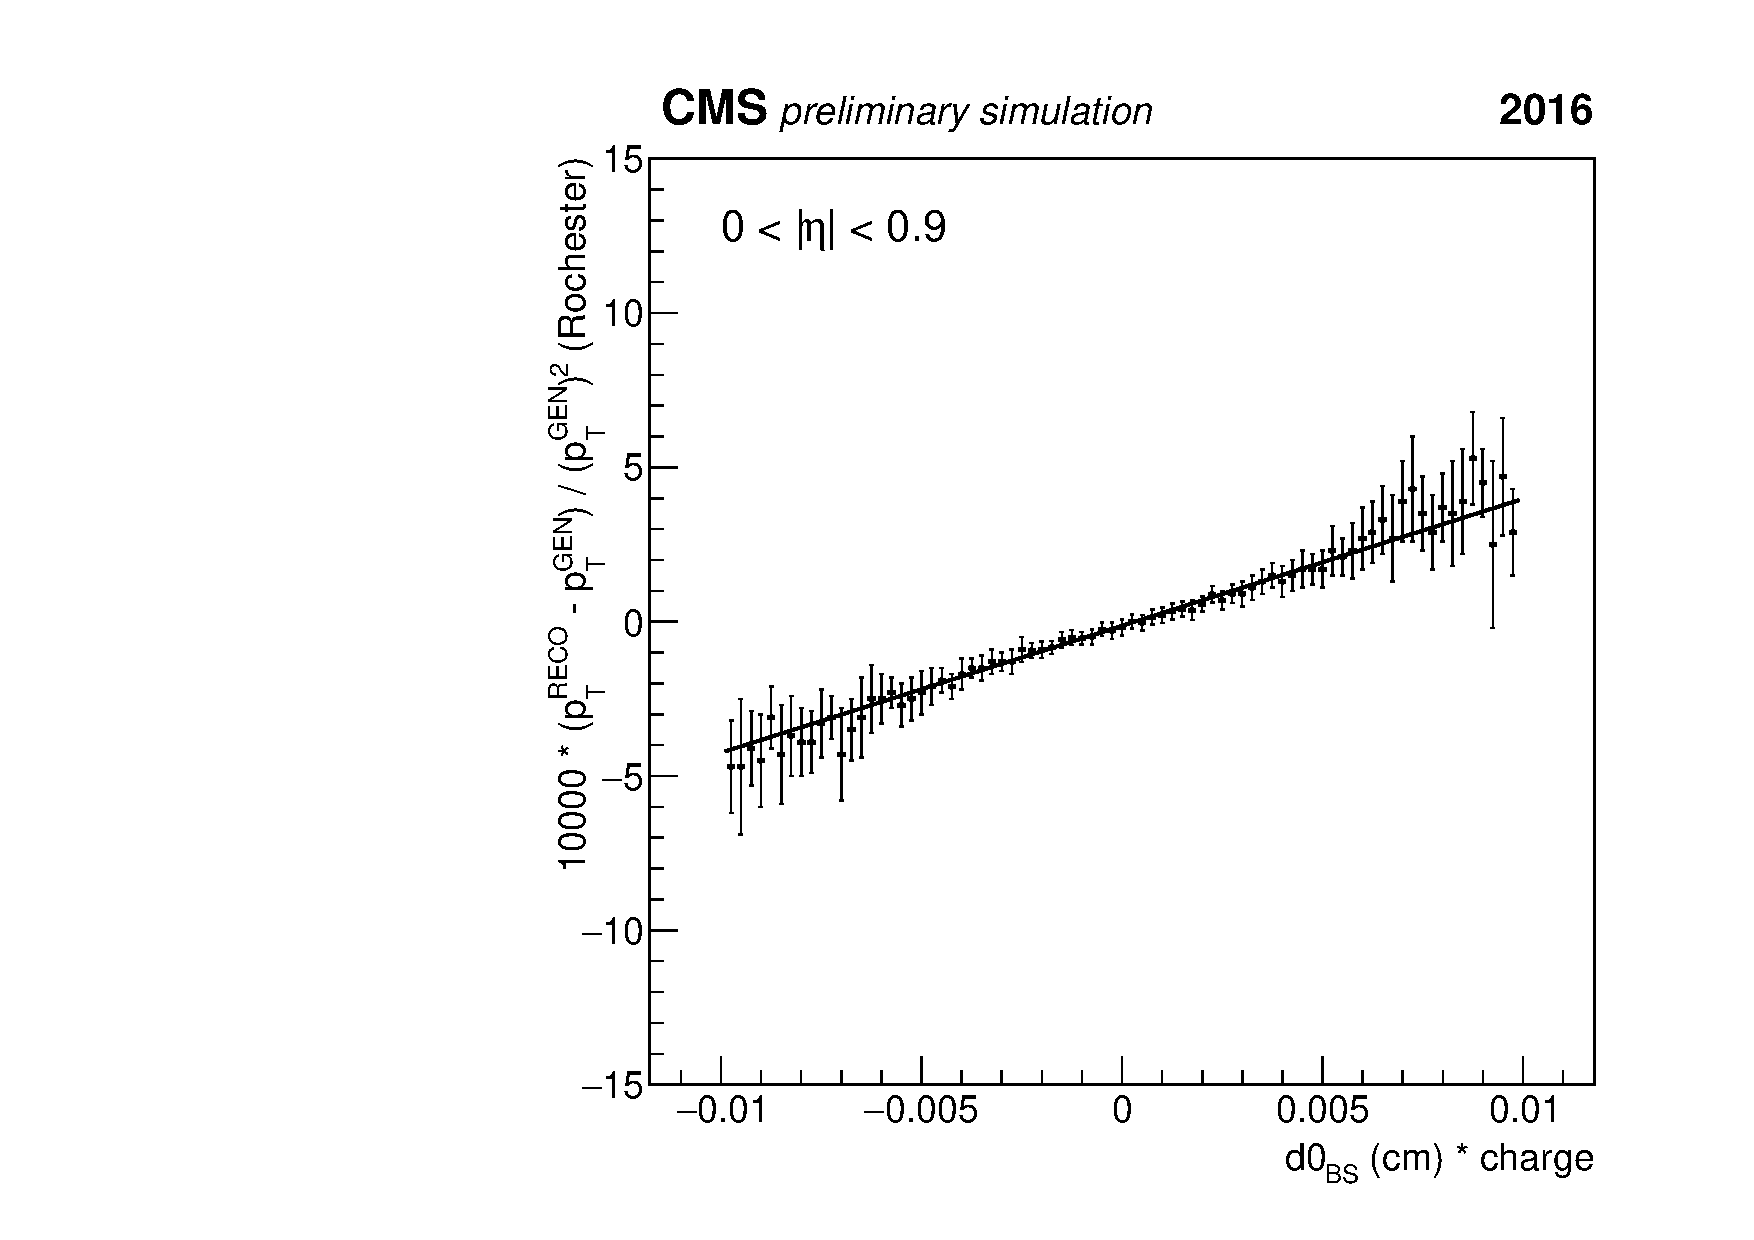
\includegraphics[width=0.49\textwidth]{images_geofit/d0_BS_dpTOverpT2_eta_0_0p9.pdf}
    \caption{Plots showing the dependence of \dptoverptsquare on \dzeroPV (left) and \dzeroBS (right). The dependence is clearly non-linear for \dzeroPV while being linear for \dzeroBS.}
    \label{fig:d0_dpTOverpT2_inclusive}
\end{figure}

After deciding which d0 definition to use, it is still necessary to understand if these corrections are correlated with other event parameters. Figures~\ref{fig:2D_d0_eta} show the dependence of the dimuon mass peak shift vs muon $\eta$. As can be seen from these plots this effect is more pronounced in higher $\eta$ regions compared to lower $\eta$ regions and that this relationship is consistent between data and MC. Figures~\ref{fig:2D_d0_eta} suggest that when deriving the constant of proportionality for \textit{GeoFit Corrections} we need to consider three separate $\eta$ regions: $|\eta| < 0.9$, $0.9 < |\eta| < 1.7$, and $|\eta| > 1.7$.  

\begin{figure}[h!]
    \centering
    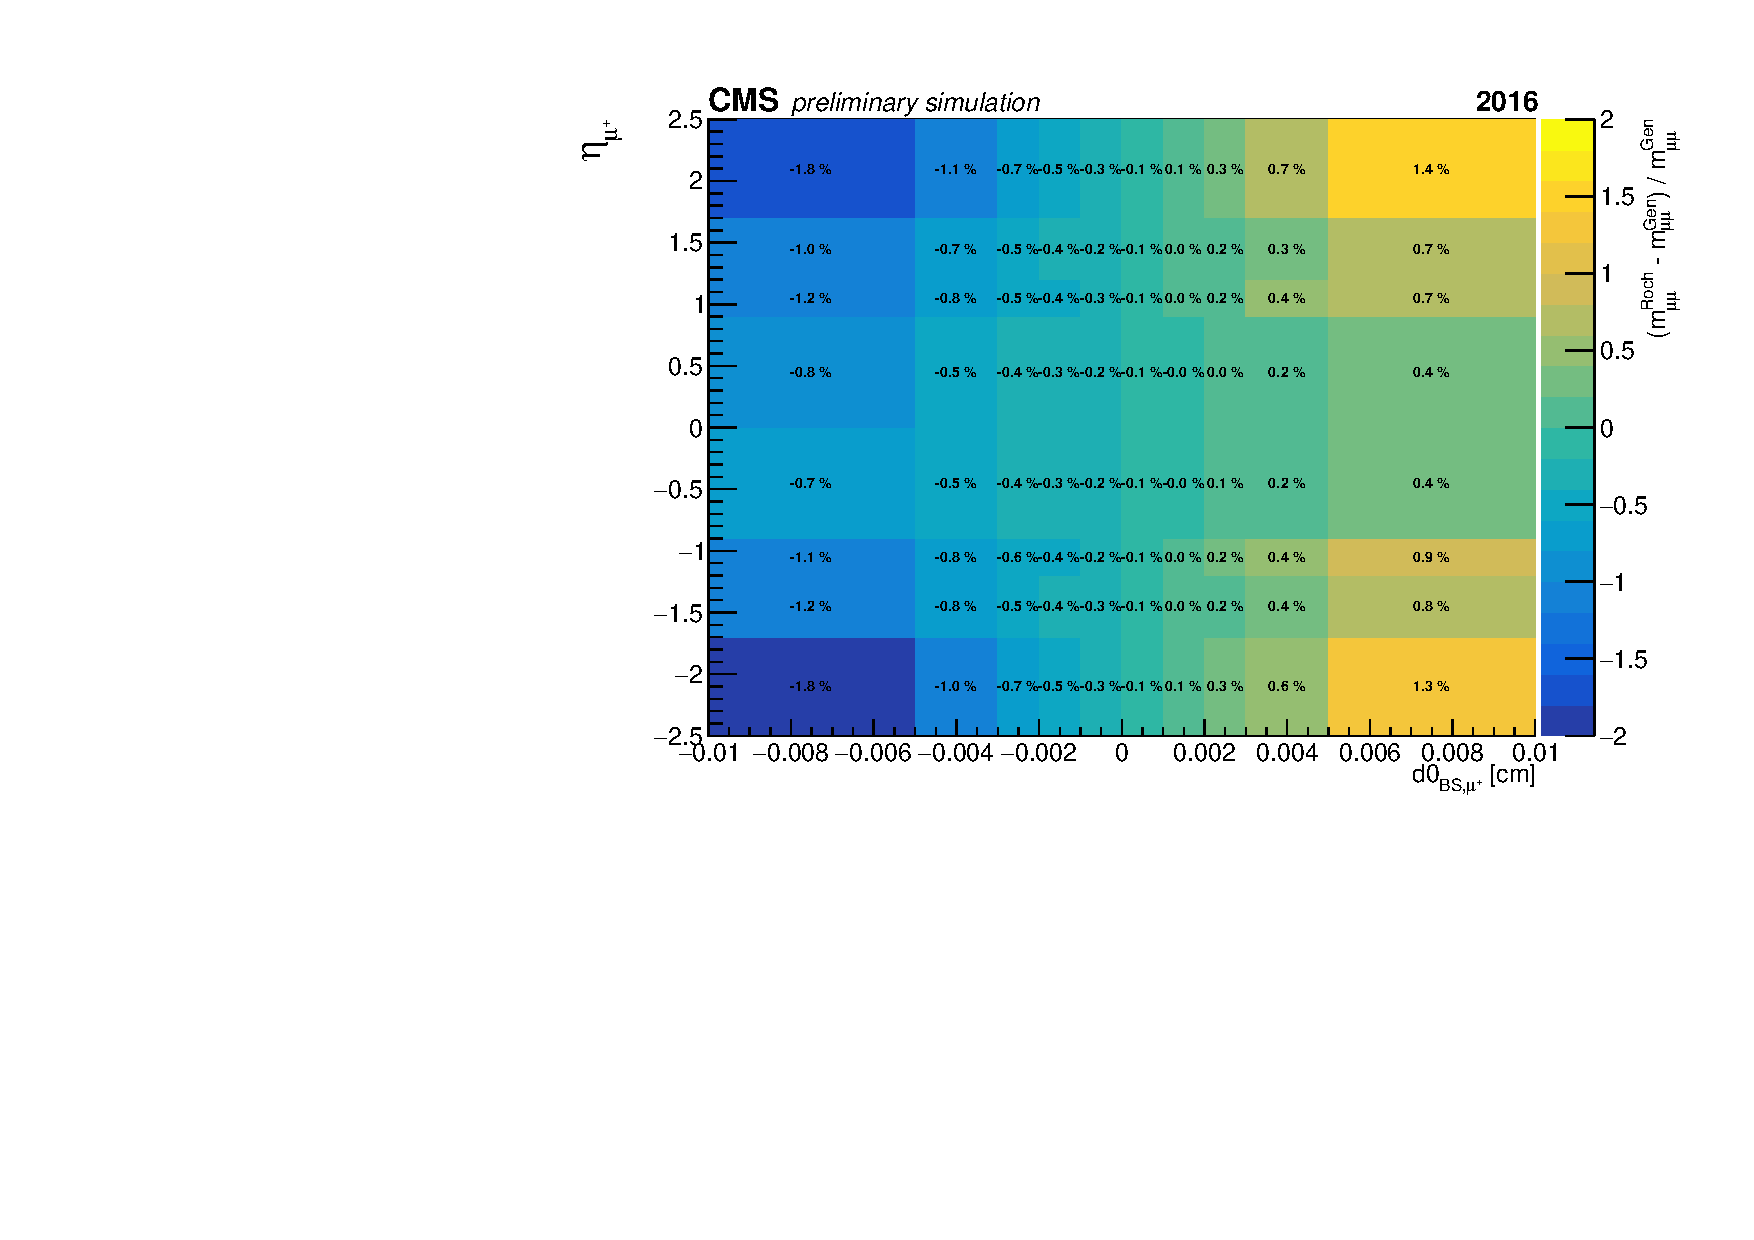
\includegraphics[width=0.49\textwidth]{images_geofit/dimu_mass_vs_eta_MC.pdf}
    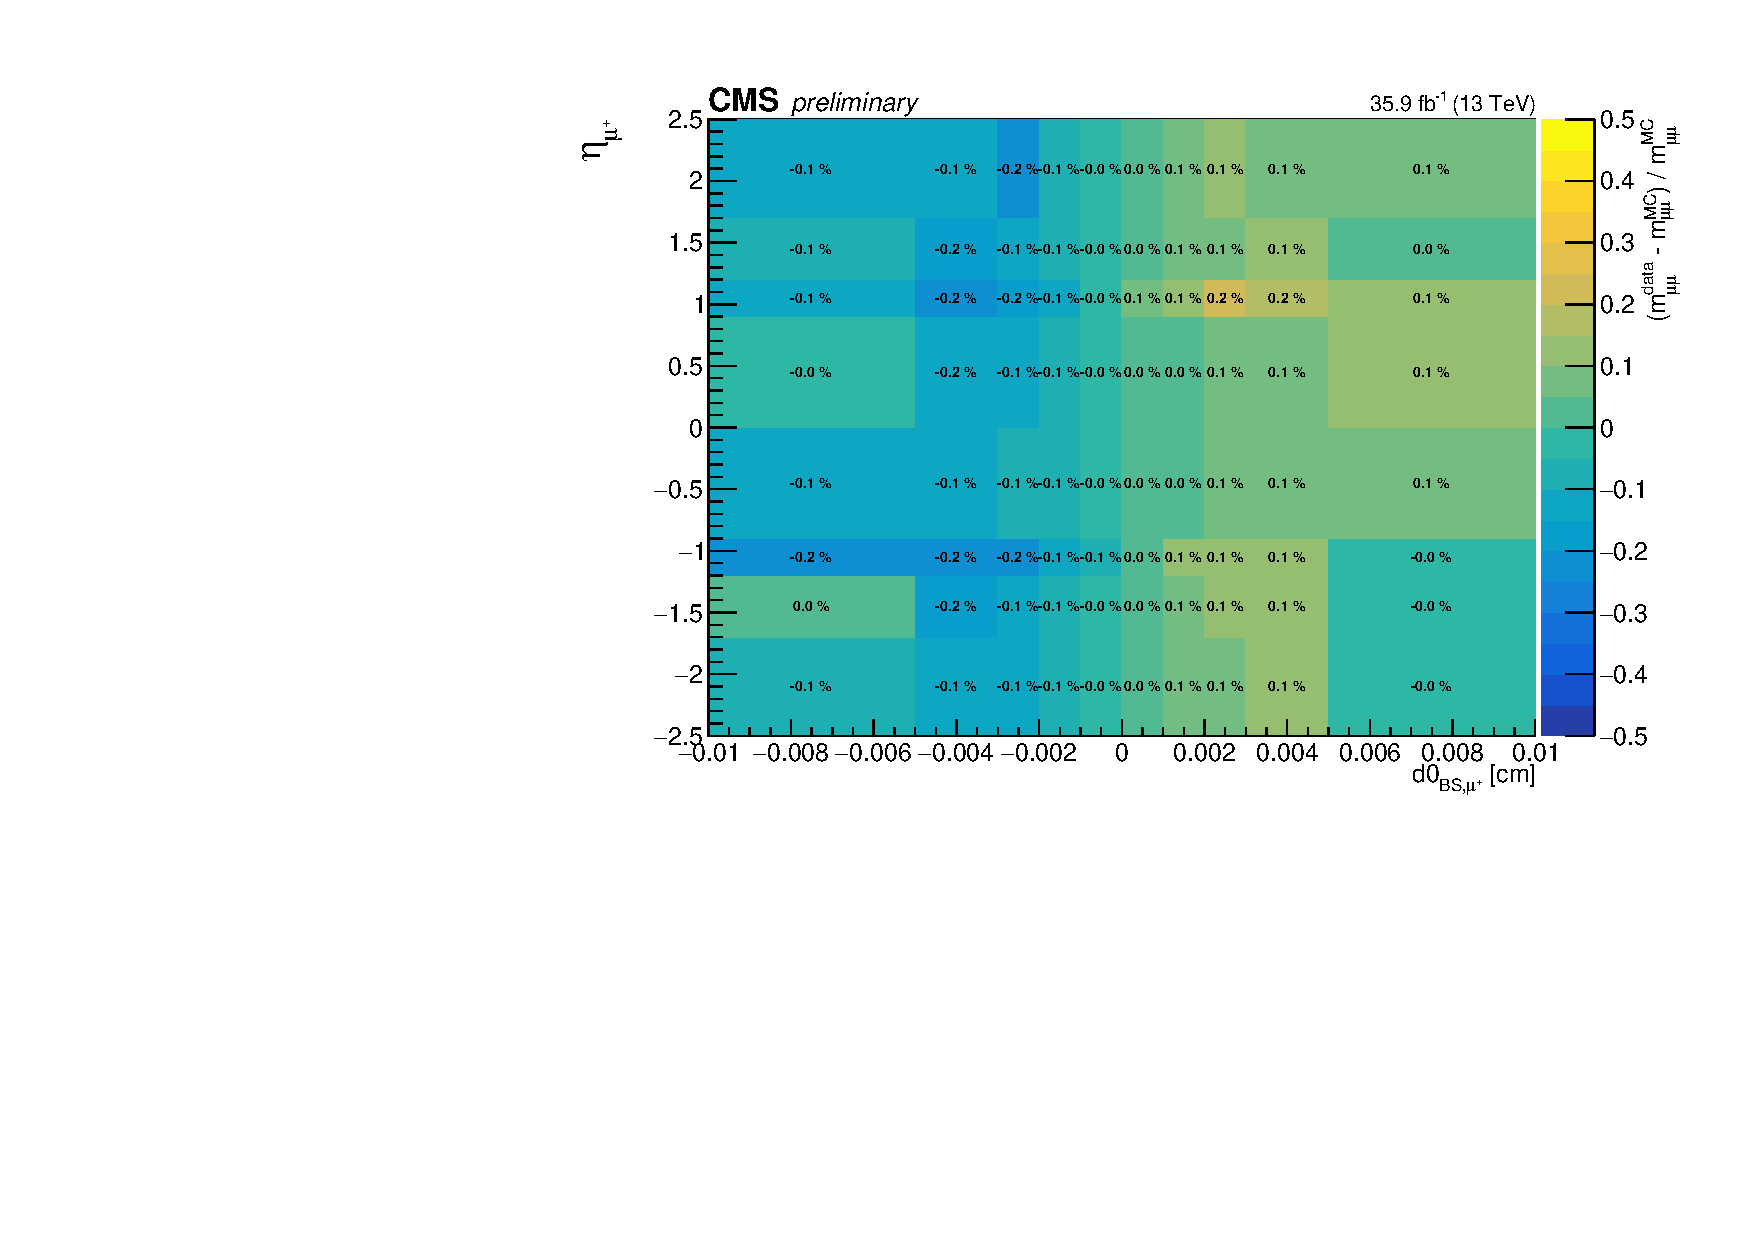
\includegraphics[width=0.49\textwidth]{images_geofit/dimu_mass_vs_eta_data.pdf}
    \caption{Plots showing the dependence of d0 effect on muon $\eta$. The d0 effect becomes more pronounced as $\eta$ increases.}
    \label{fig:2D_d0_eta}
\end{figure}

Figures~\ref{fig:2D_d0_phi} show the dependence of the dimuon mass peak shift vs muon $\phi$. The d0 effect on \pt seems to be independent of muon $\phi$ and therefore we do not need to consider different regions of $\phi$.

\begin{figure}[h!]
    \centering
    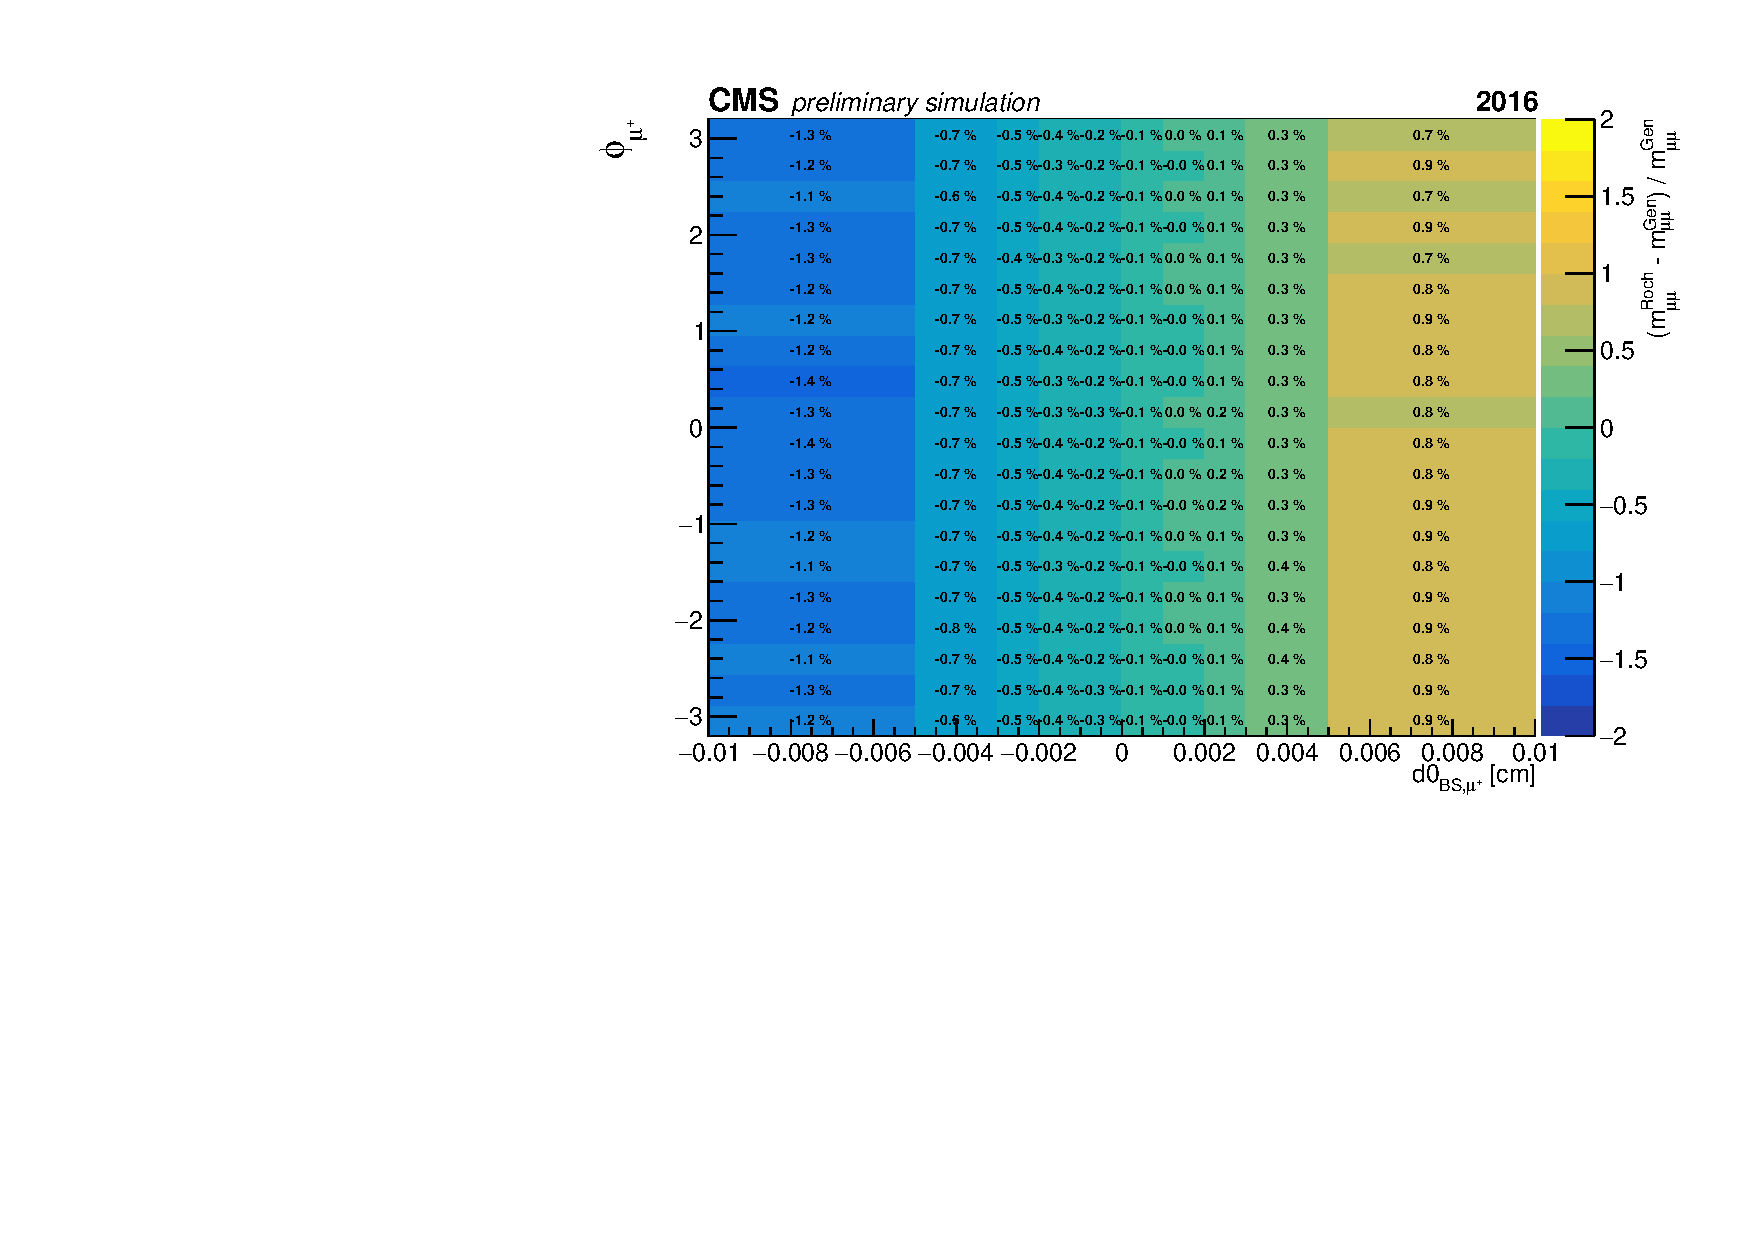
\includegraphics[width=0.49\textwidth]{images_geofit/dimu_mass_vs_phi_MC.pdf}
    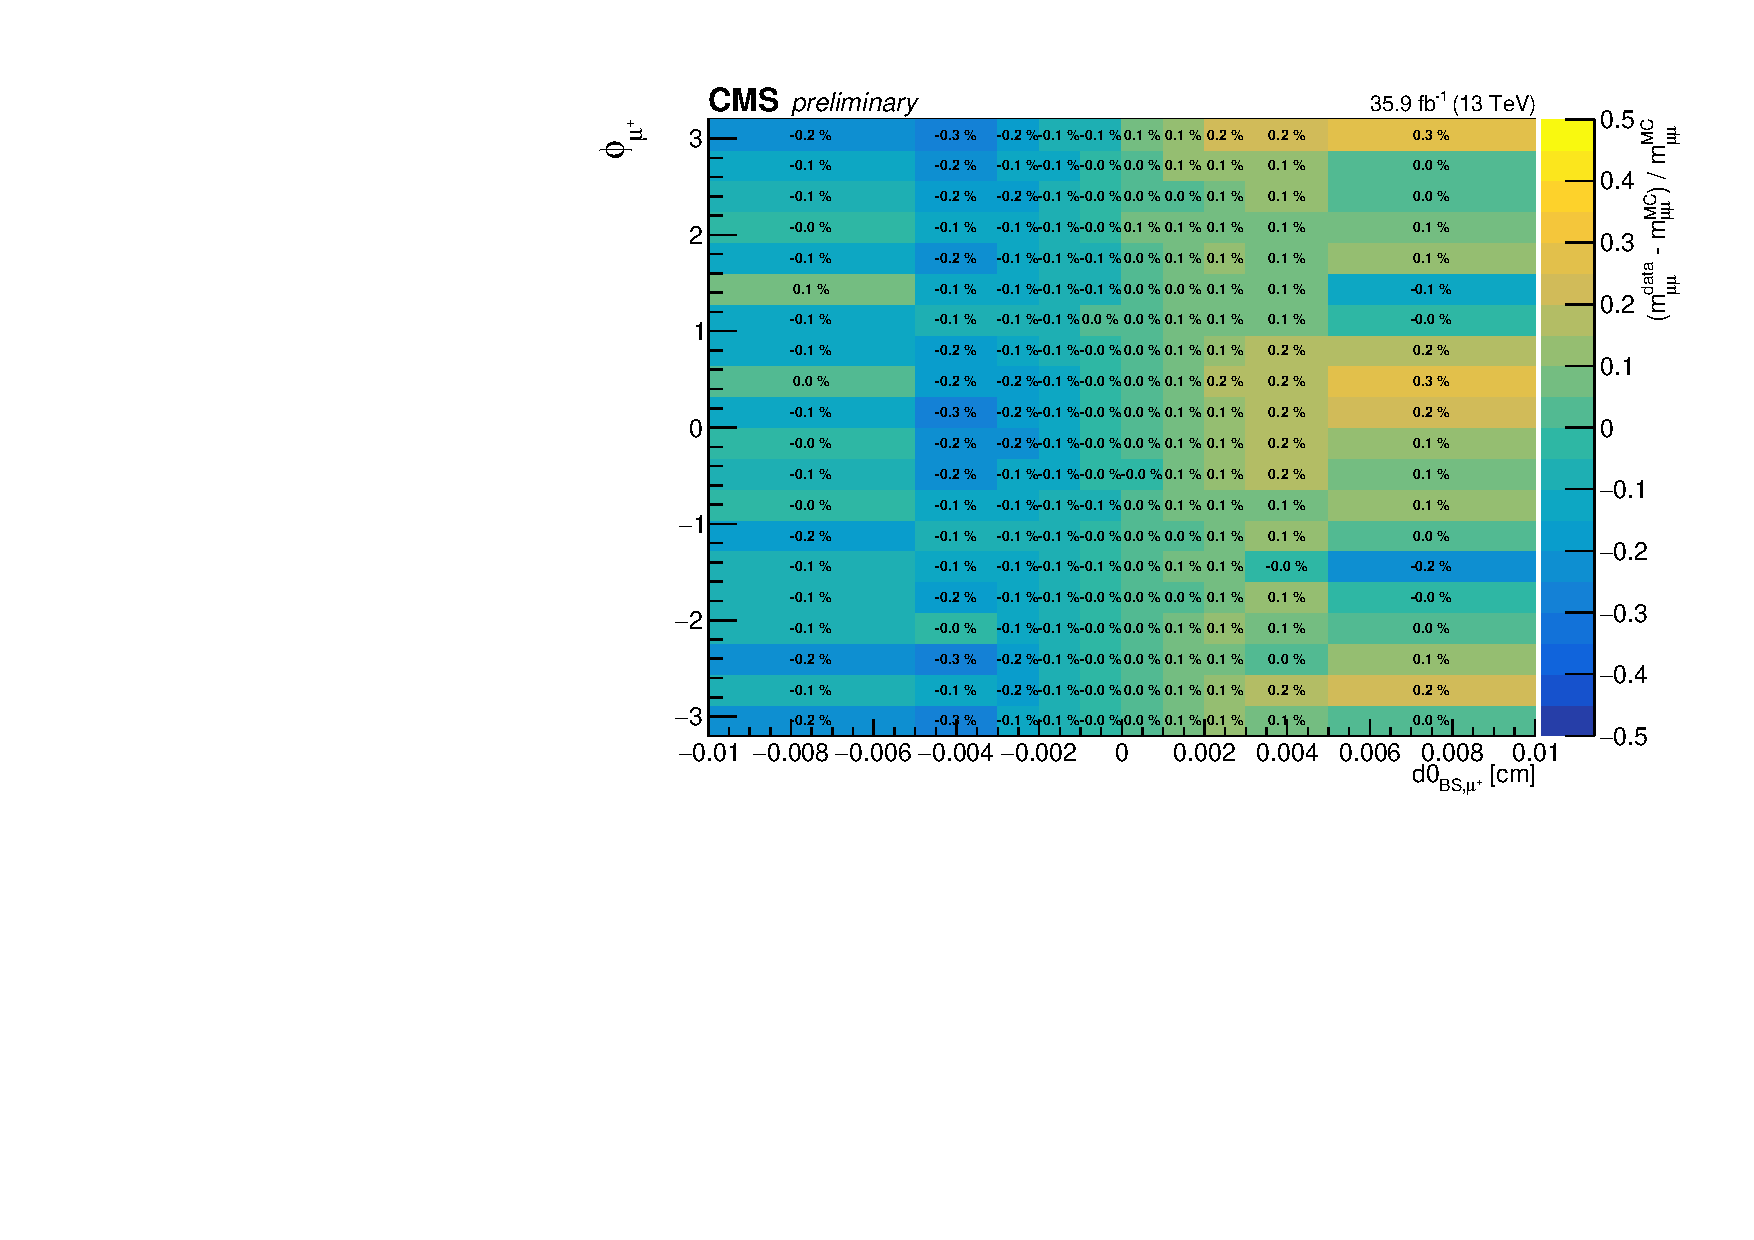
\includegraphics[width=0.49\textwidth]{images_geofit/dimu_mass_vs_phi_data.pdf}
    \caption{Plots showing the dependence of d0 effect on muon $\phi$. There is no clear dependence on $\phi$.}
    \label{fig:2D_d0_phi}
\end{figure}

The remaining studies are done by using \dptoverptsquare vs. \dzeroBS distributions in the three $|\eta|$ regions defined above.

Figures~\ref{fig:nVtx_d0_2016},~\ref{fig:nVtx_d0_2017} and ~\ref{fig:nVtx_d0_2018} show the dependence of \textit{GeoFit Corrections} on pileup. The constant of proportionality derived from events with low number of vertices in the event is consistent with the constant of proportionality derived from events with high number of vertices. Therefore it is understood that \textit{GeoFit Corrections} do not depend on the amount of pileup in the event.

\begin{figure}[h!]
    \centering
    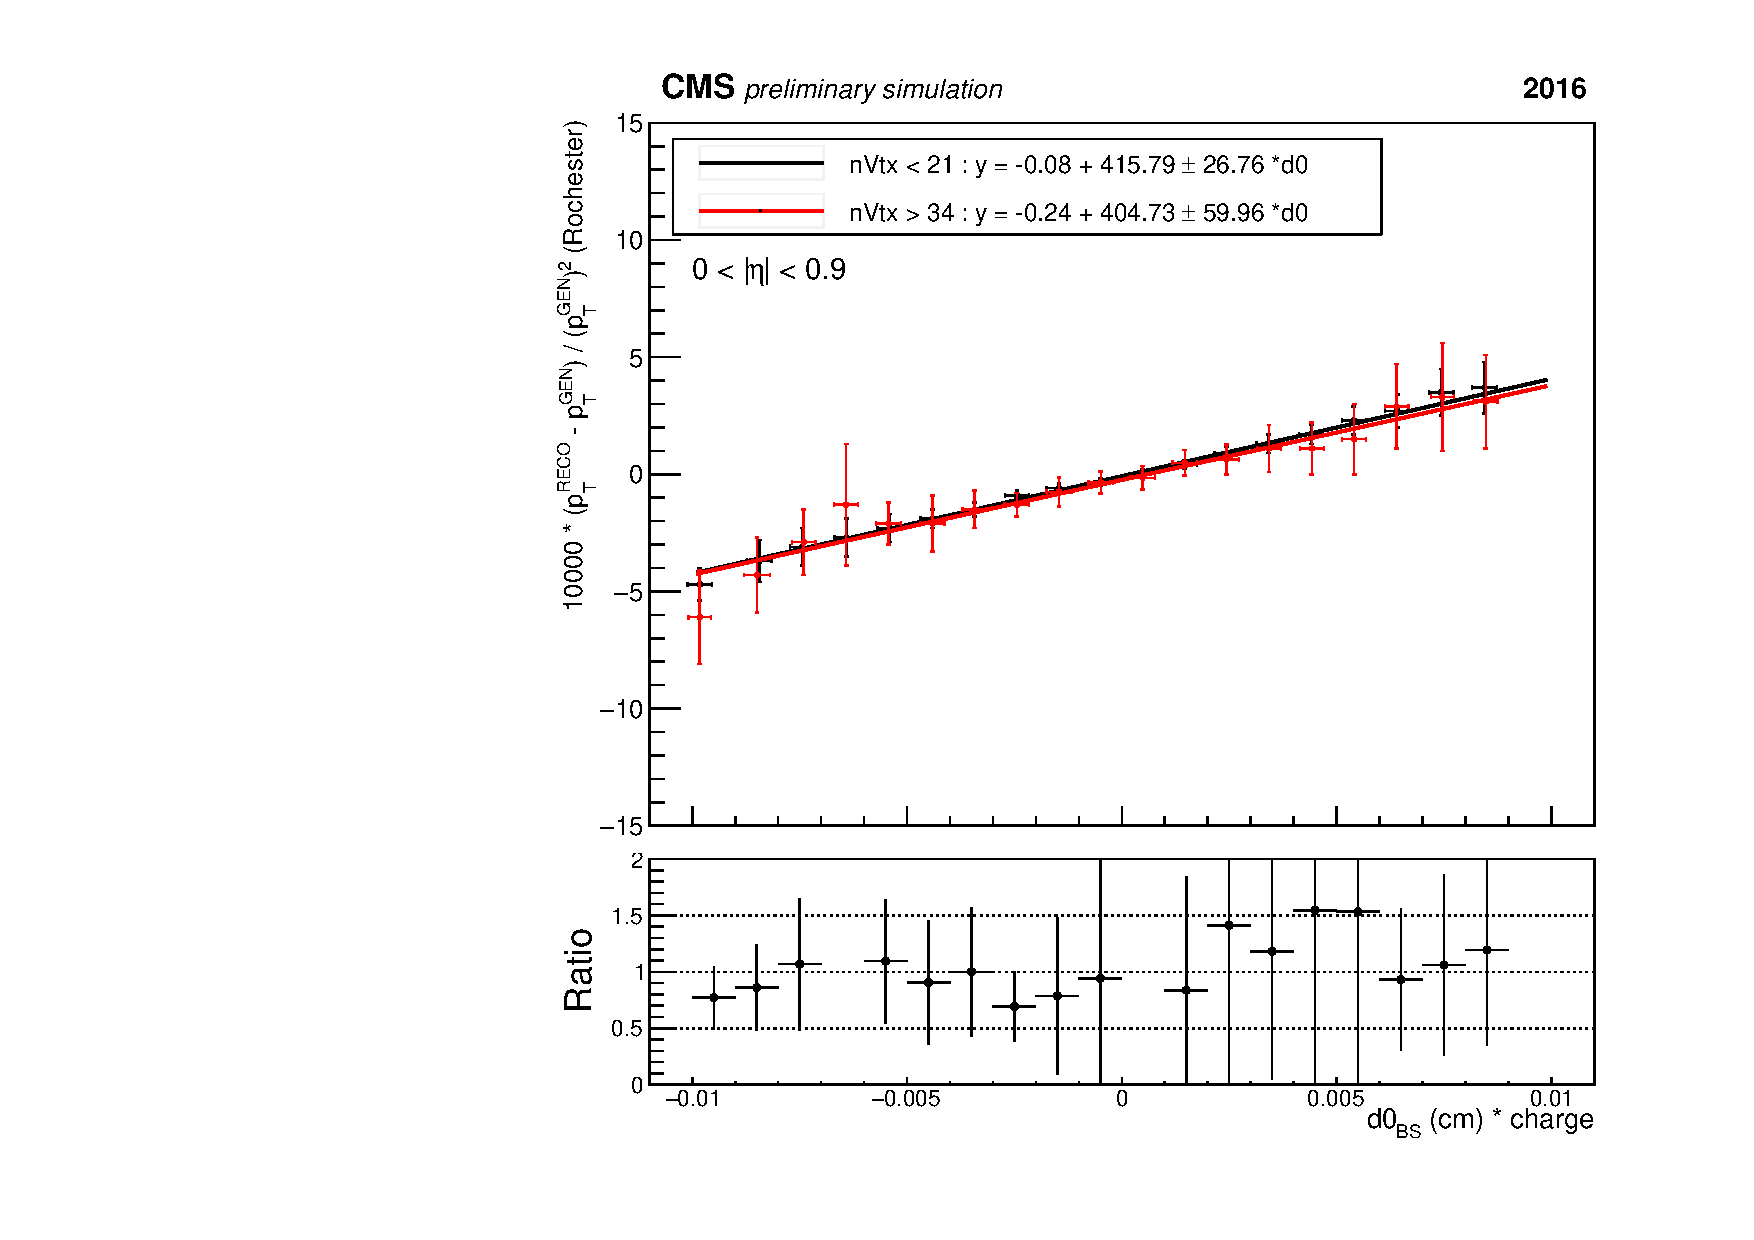
\includegraphics[width=0.32\textwidth]{images_geofit/nVtx_eta_0_0p9_2016.pdf}
    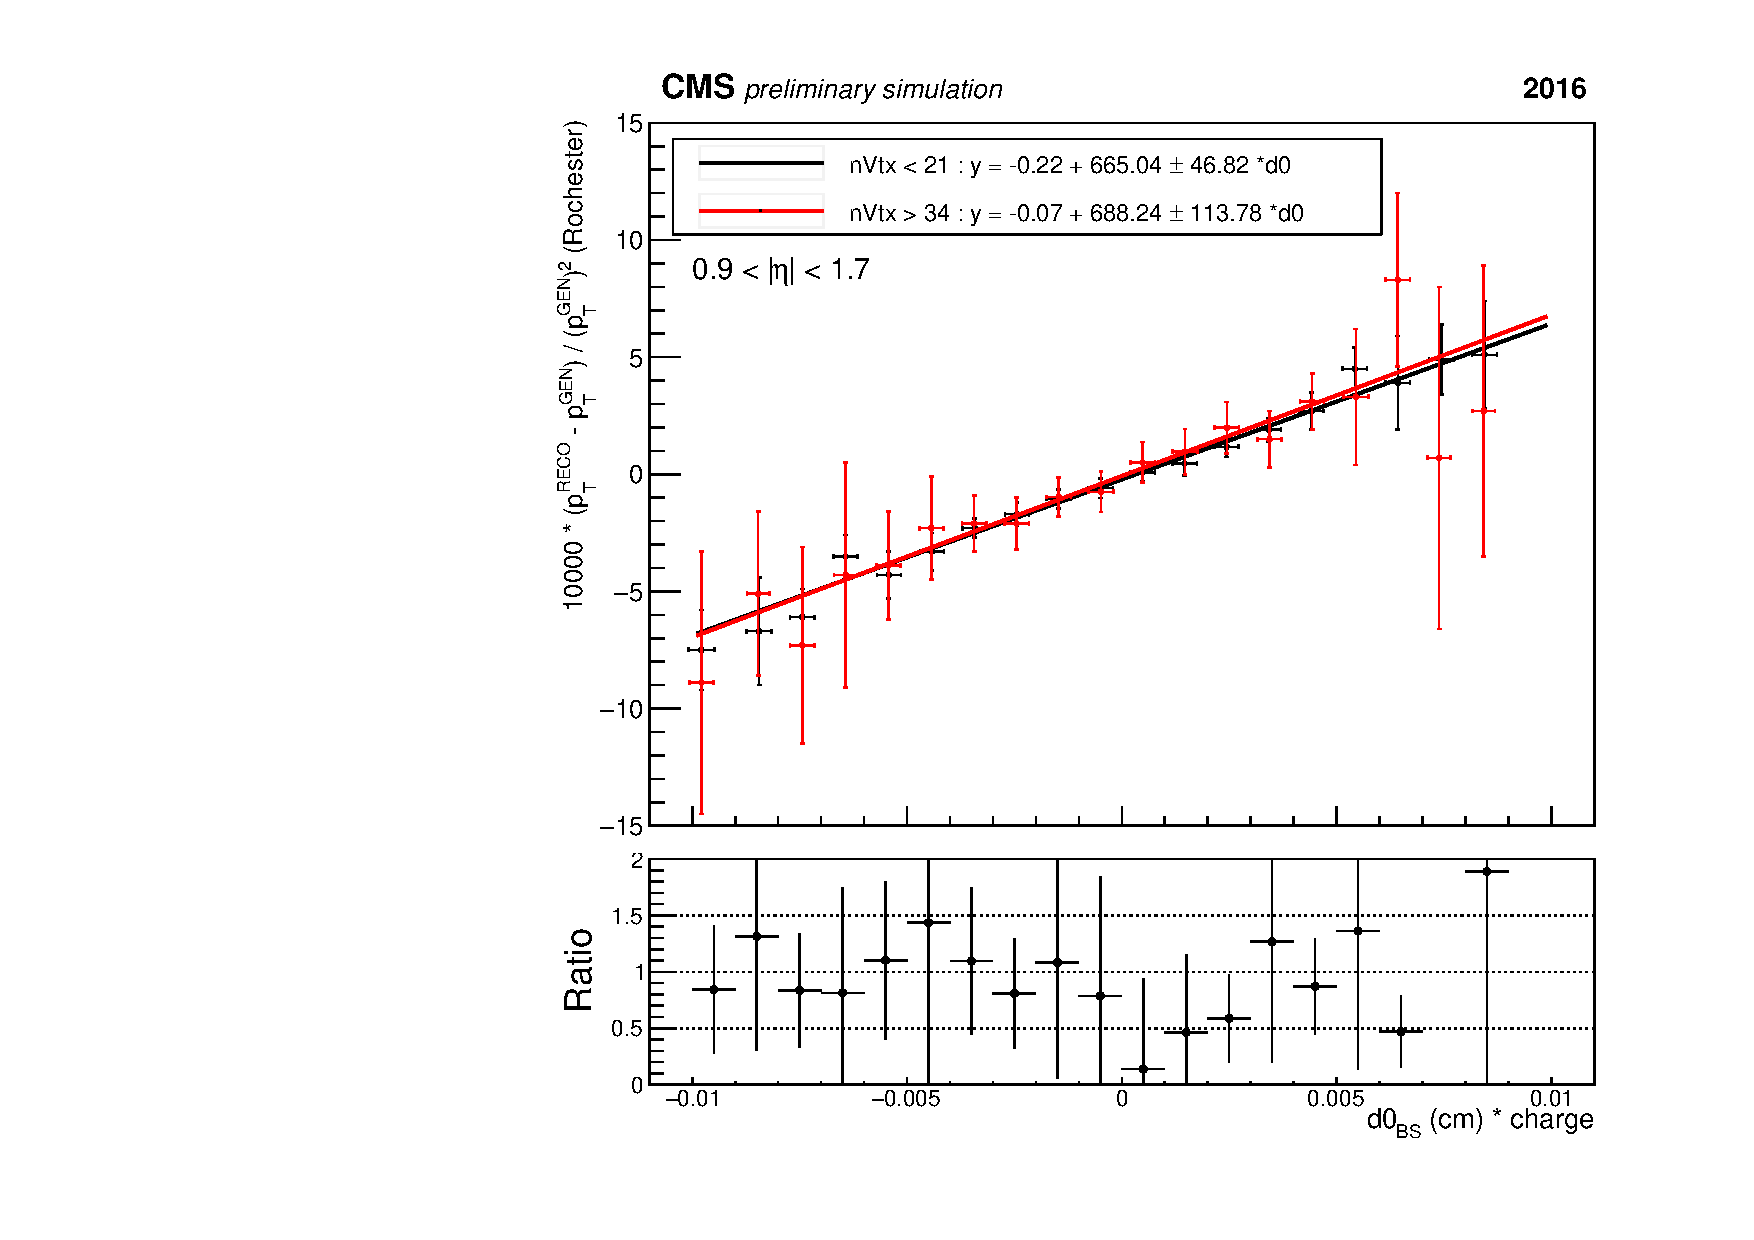
\includegraphics[width=0.32\textwidth]{images_geofit/nVtx_eta_0p9_1p7_2016.pdf}
    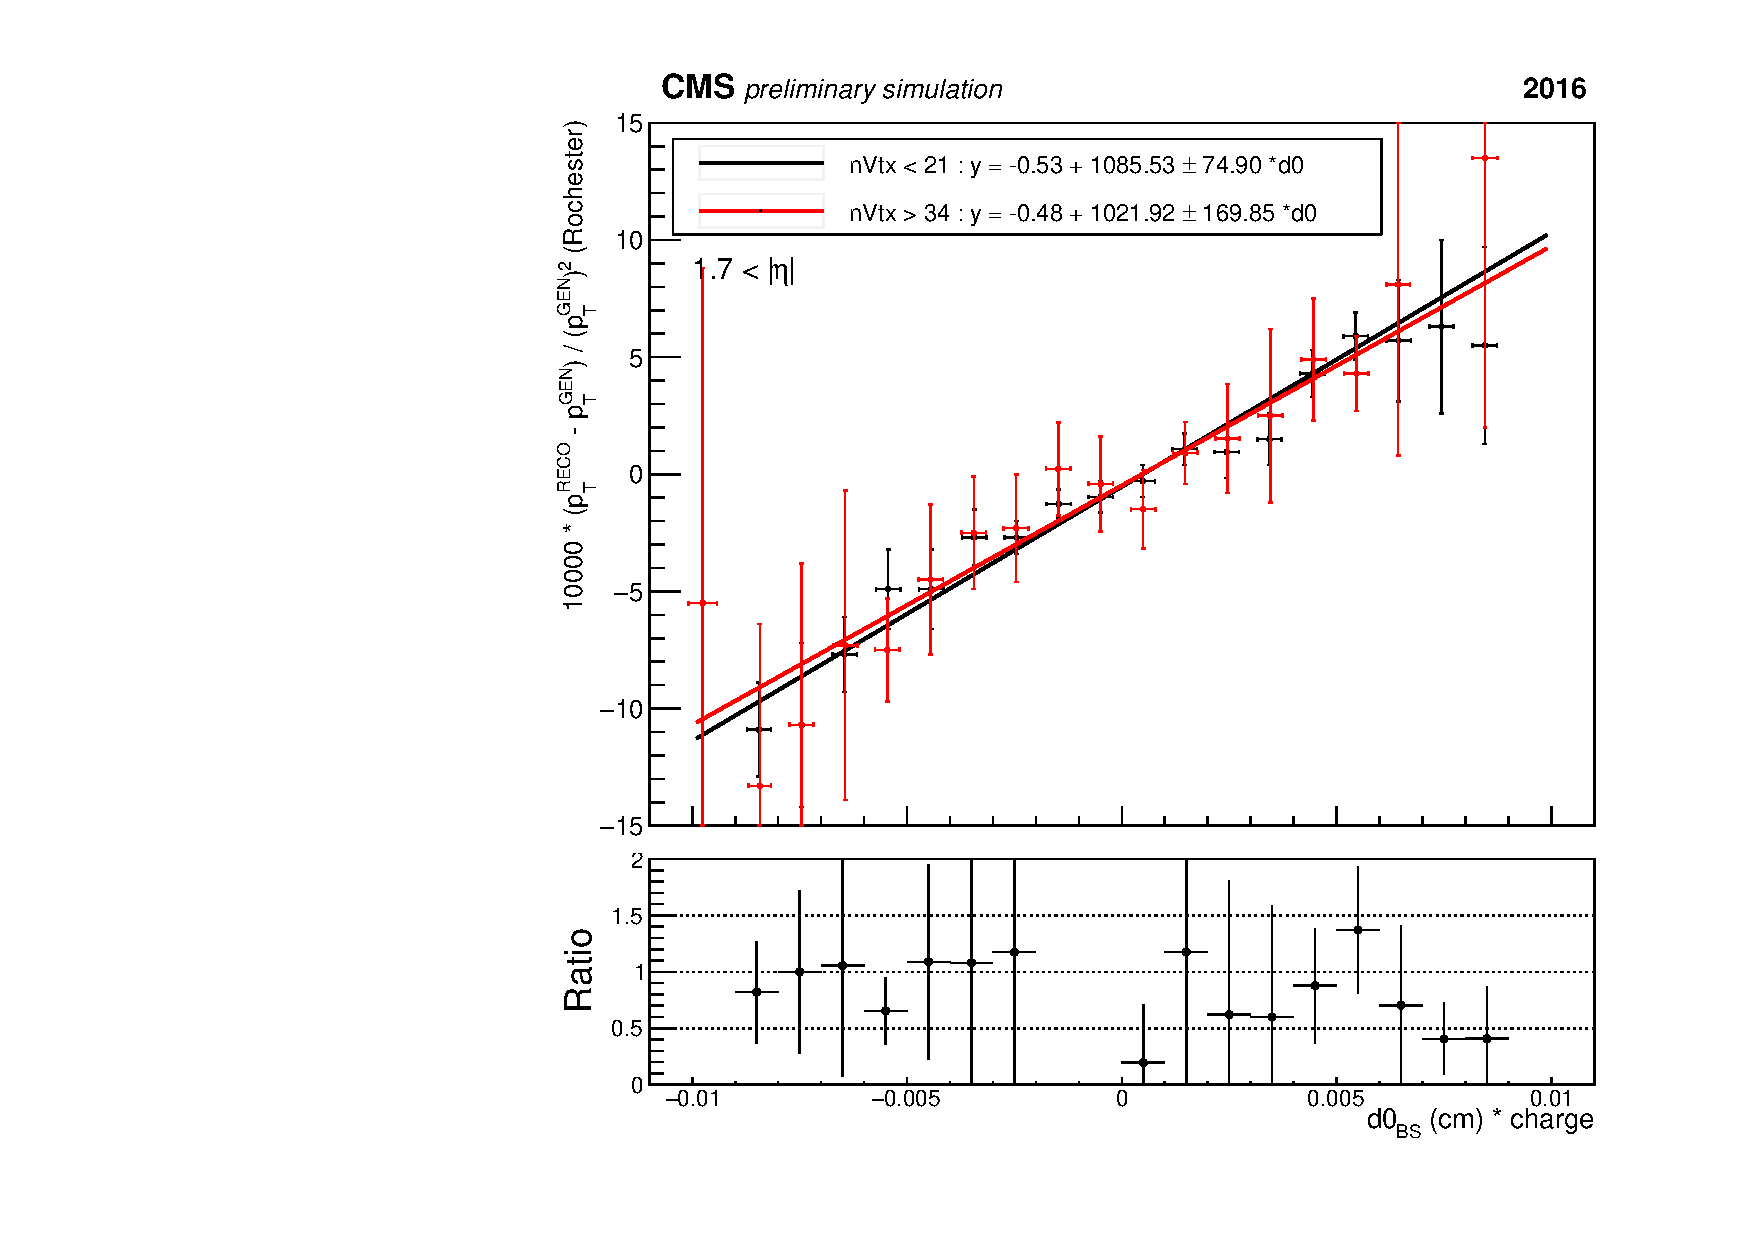
\includegraphics[width=0.32\textwidth]{images_geofit/nVtx_eta_1p7_inf_2016.pdf}
    \caption{Plots comparing \dptoverptsquare vs \dzeroBS distributions for events with number of vertices less than 21 and number of vertices more than 34 for each $|\eta|$ region derived from Z+jets MC in 2016. The ratio plot show the ratio between the black data points (nVtx $<$ 21) and the red data points (nVtx $>$ 34).}
    \label{fig:nVtx_d0_2016}
\end{figure}

\begin{figure}[h!]
    \centering
    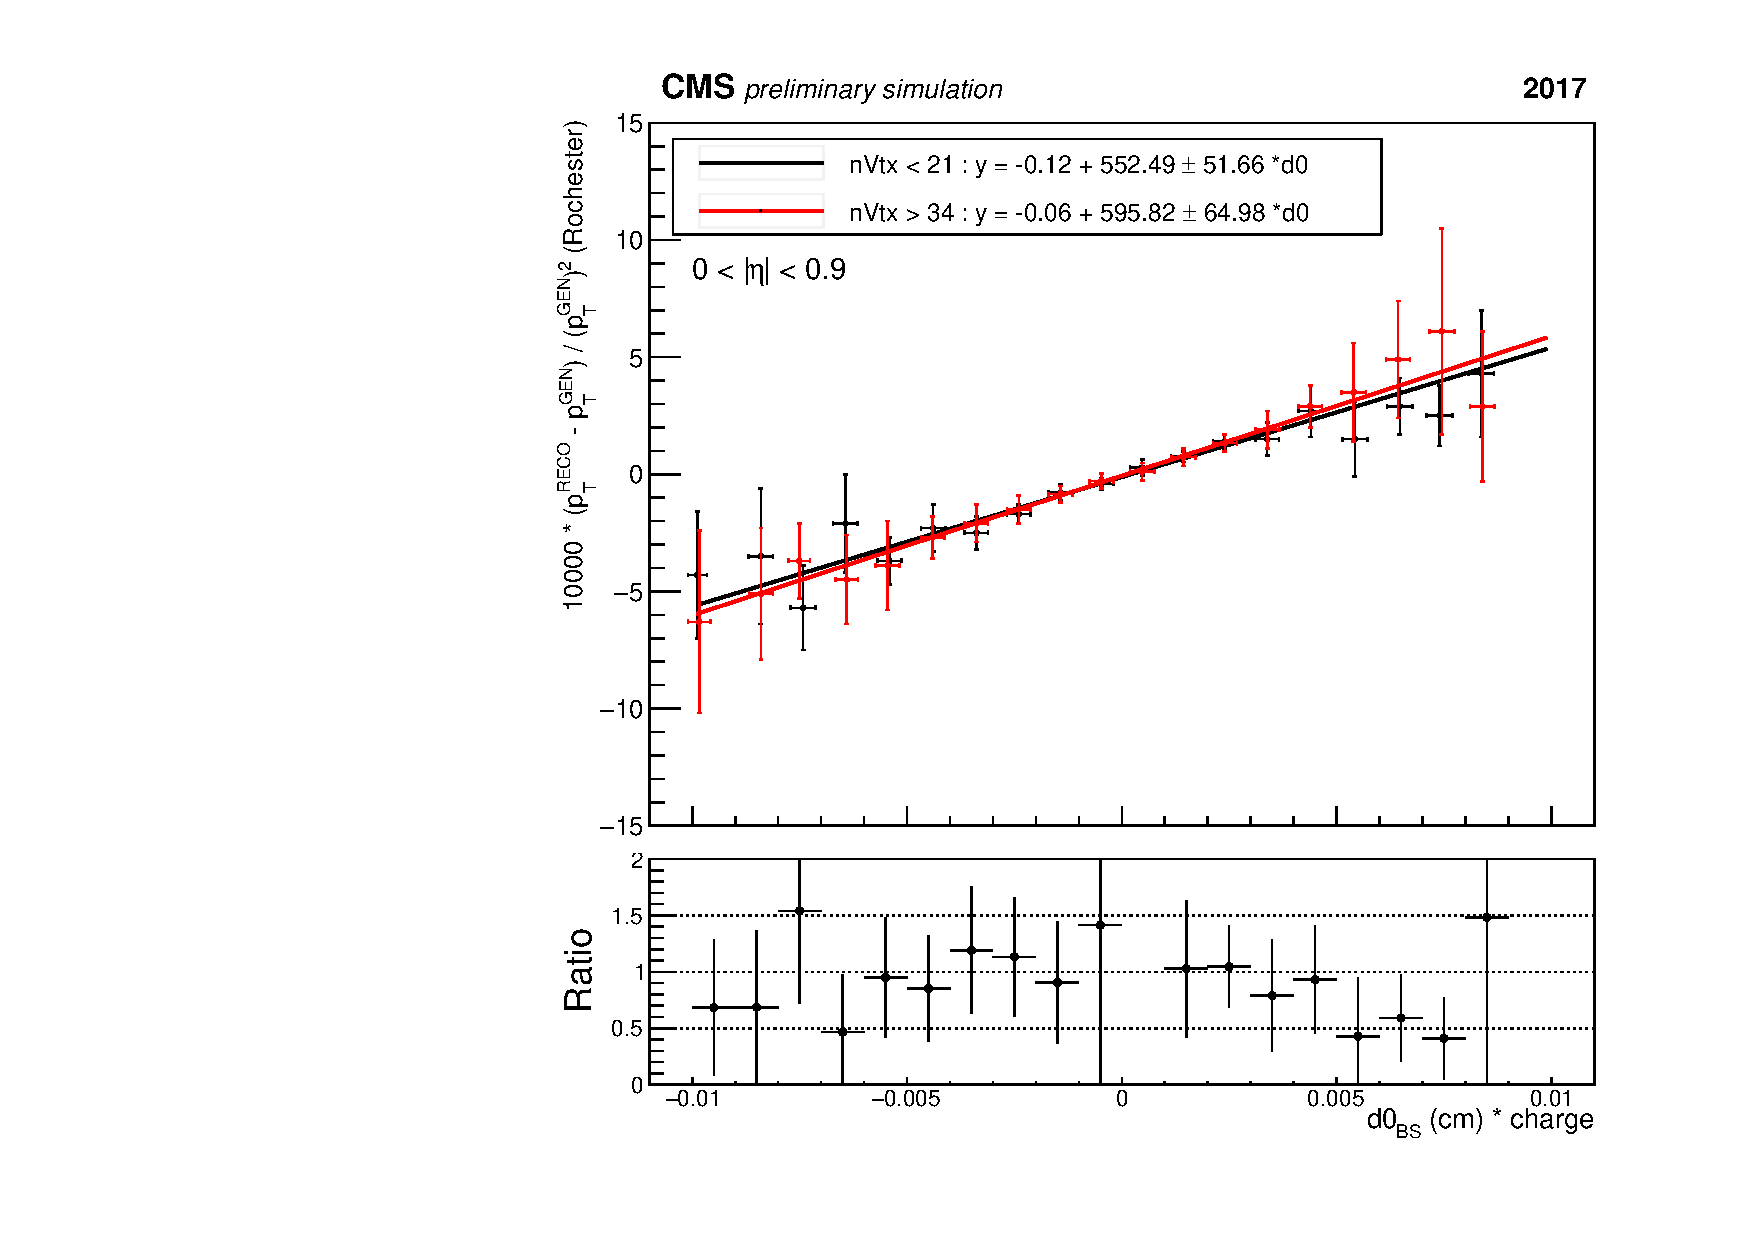
\includegraphics[width=0.32\textwidth]{images_geofit/nVtx_eta_0_0p9_2017.pdf}
    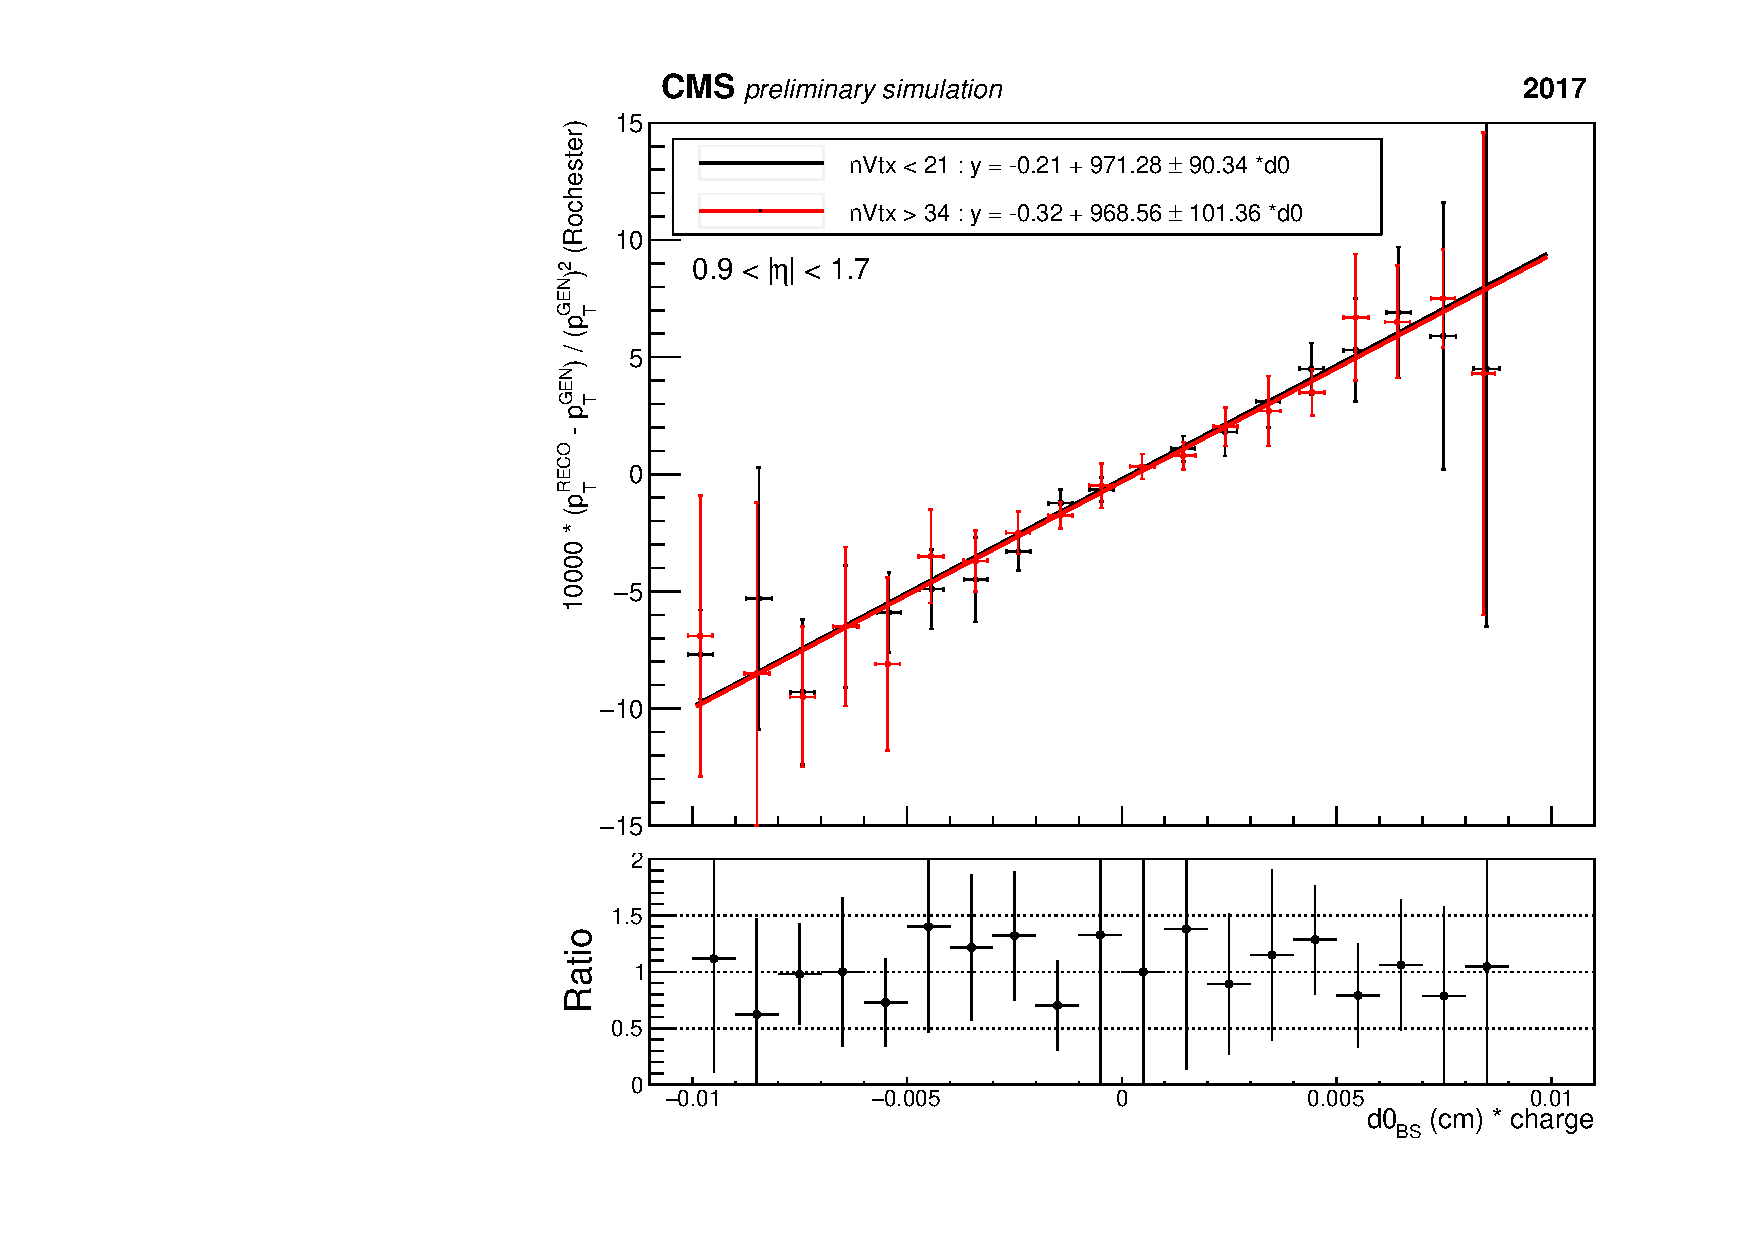
\includegraphics[width=0.32\textwidth]{images_geofit/nVtx_eta_0p9_1p7_2017.pdf}
    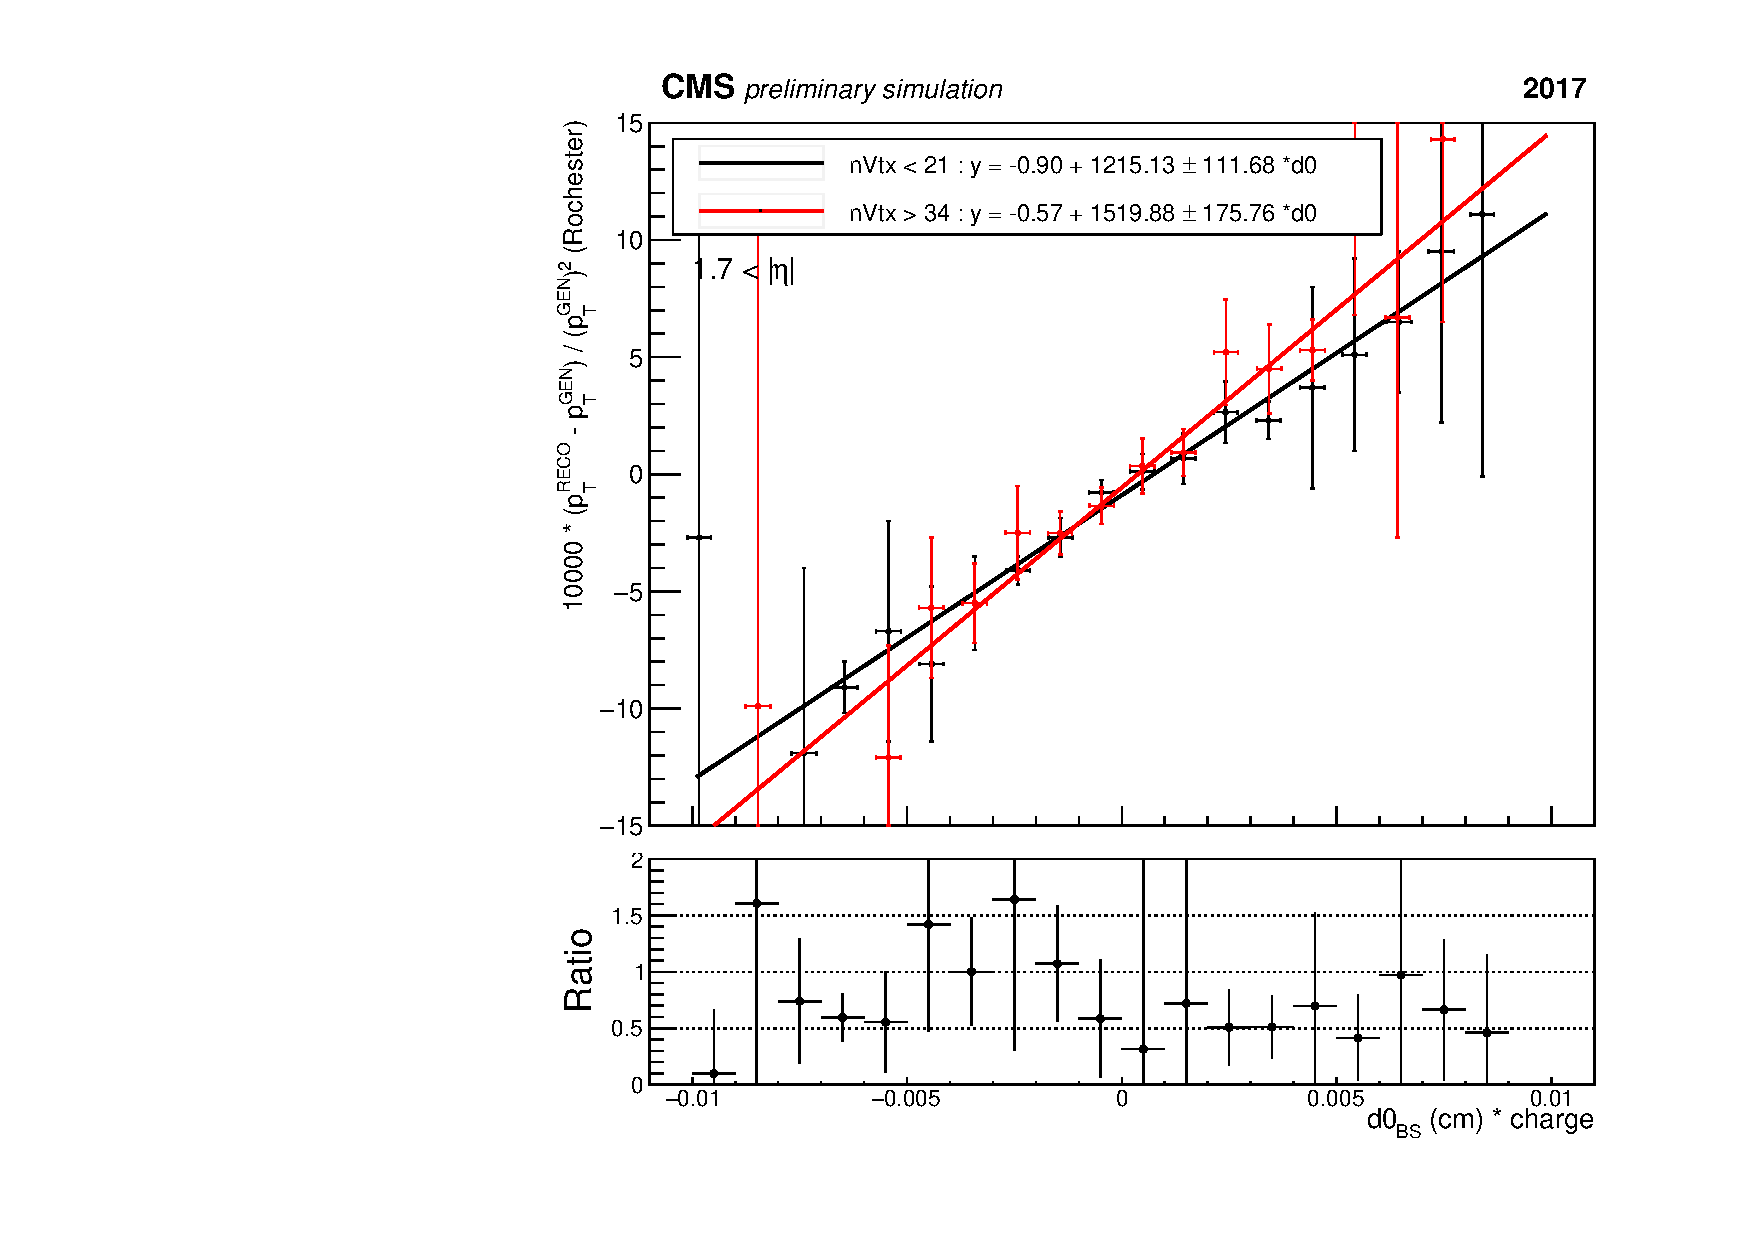
\includegraphics[width=0.32\textwidth]{images_geofit/nVtx_eta_1p7_inf_2017.pdf}
    \caption{Plots comparing \dptoverptsquare vs \dzeroBS distributions for events with number of vertices less than 21 and number of vertices more than 34 for each $|\eta|$ region derived from Z+jets MC in 2017. The ratio plot show the ratio between the black data points (nVtx $<$ 21) and the red data points (nVtx $>$ 34).}
    \label{fig:nVtx_d0_2017}
\end{figure}

\begin{figure}[h!]
    \centering
    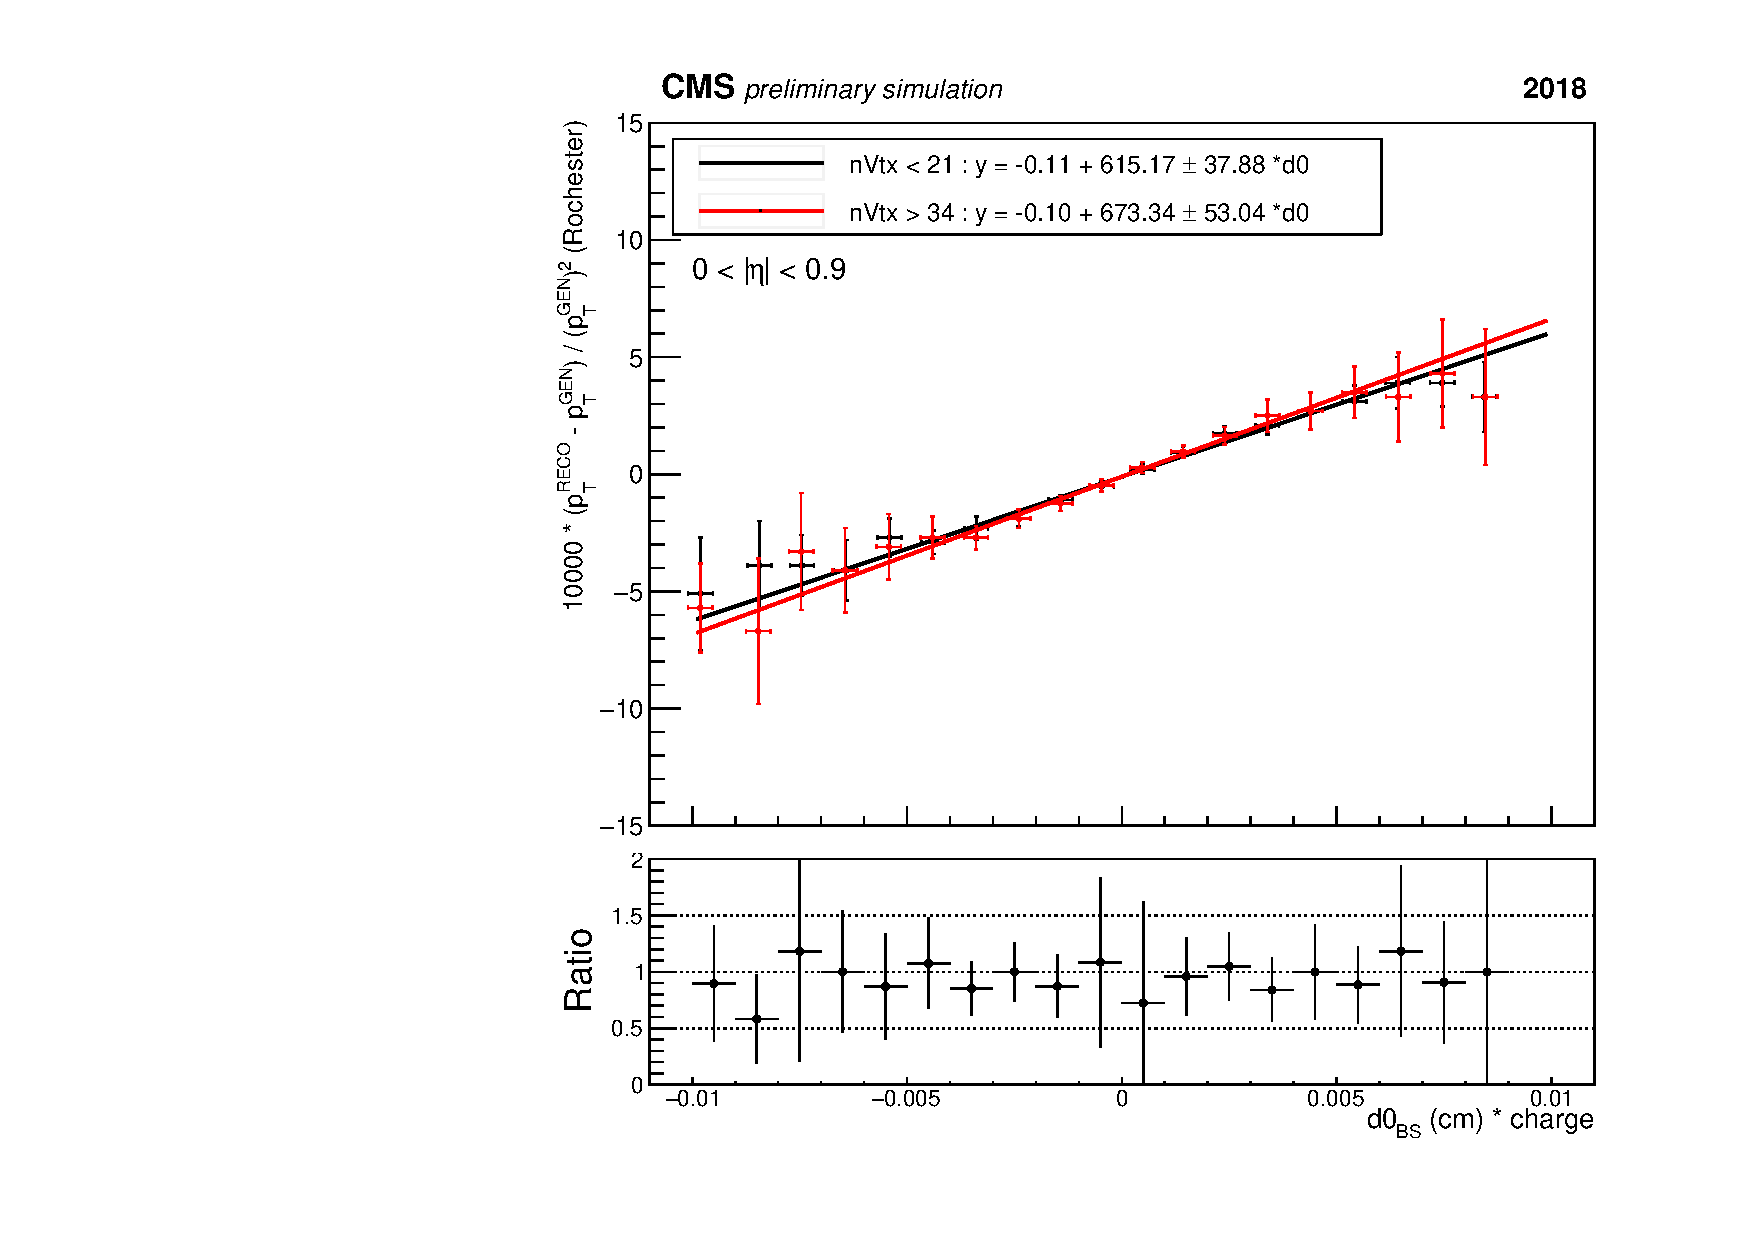
\includegraphics[width=0.32\textwidth]{images_geofit/nVtx_eta_0_0p9_2018.pdf}
    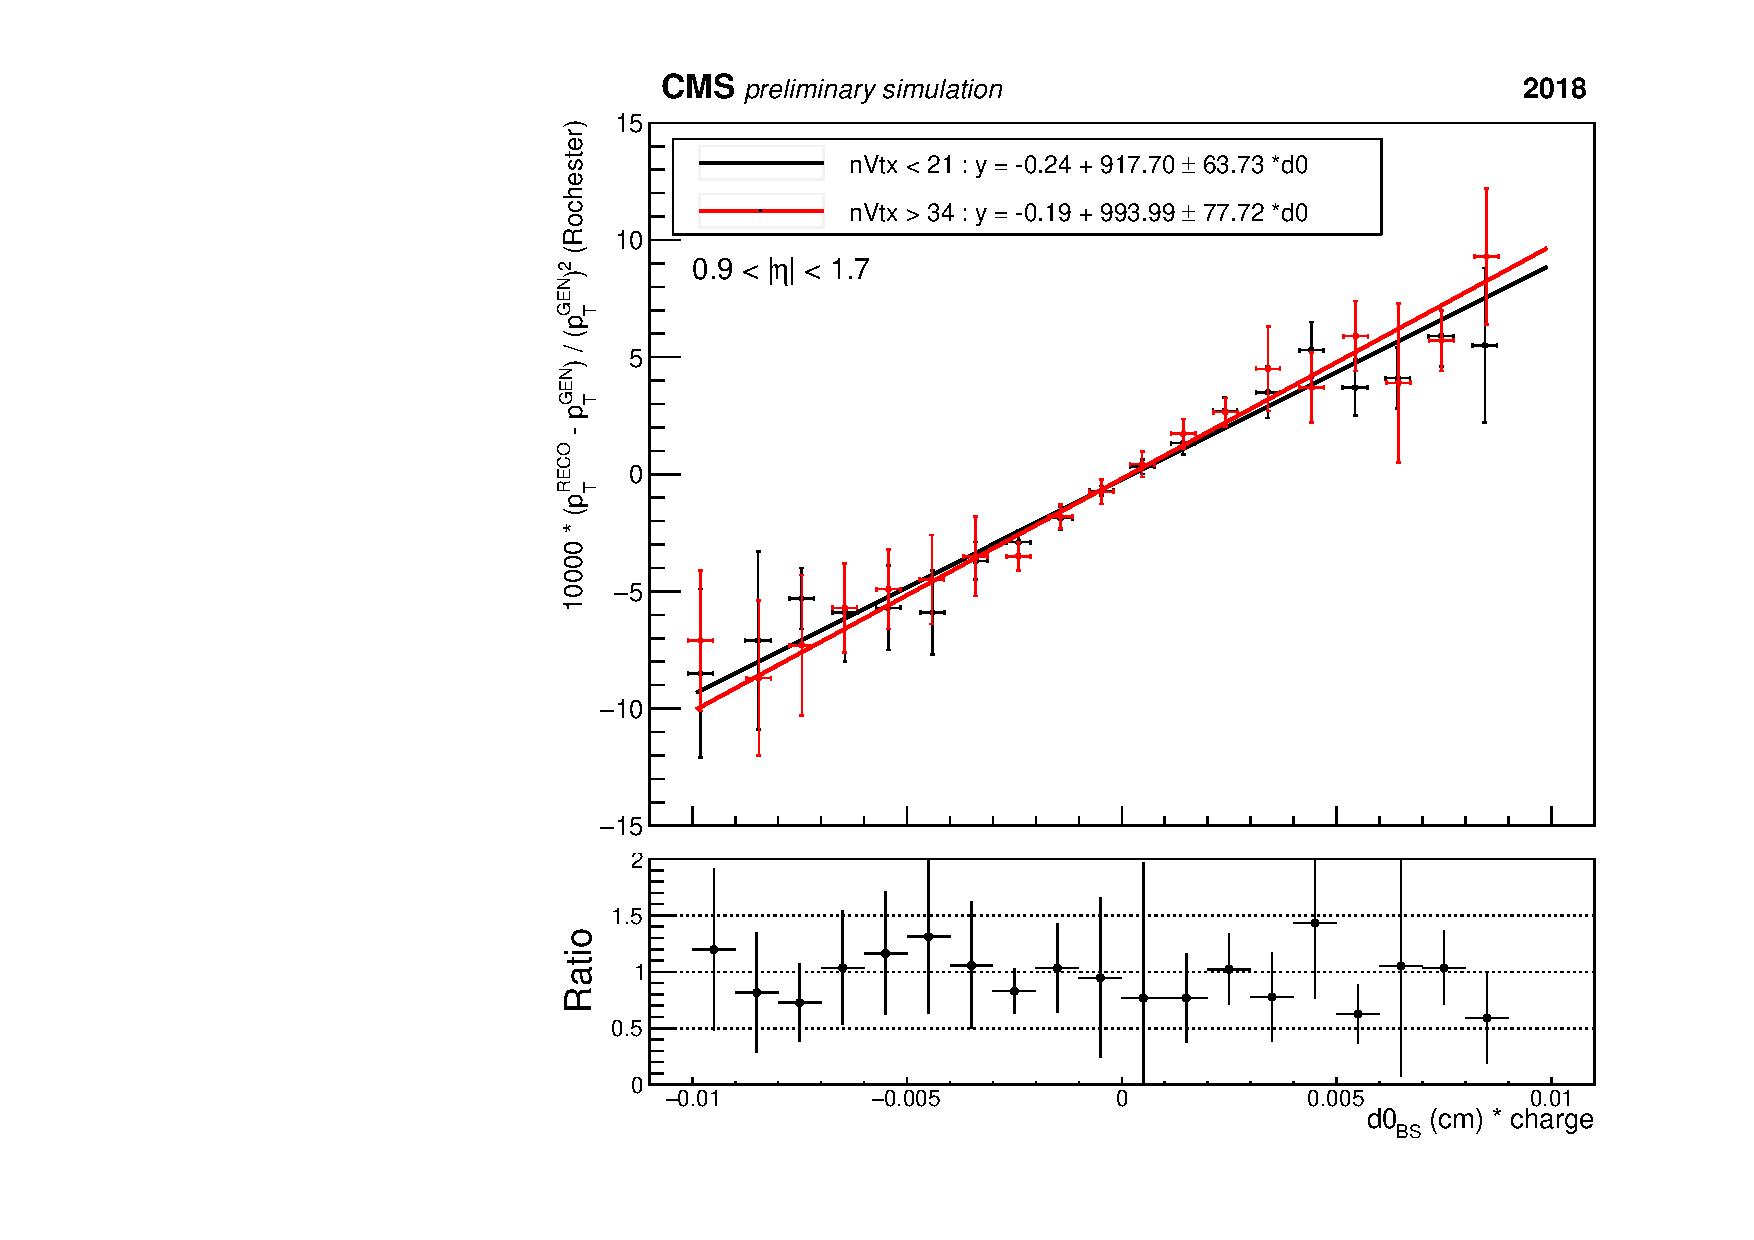
\includegraphics[width=0.32\textwidth]{images_geofit/nVtx_eta_0p9_1p7_2018.pdf}
    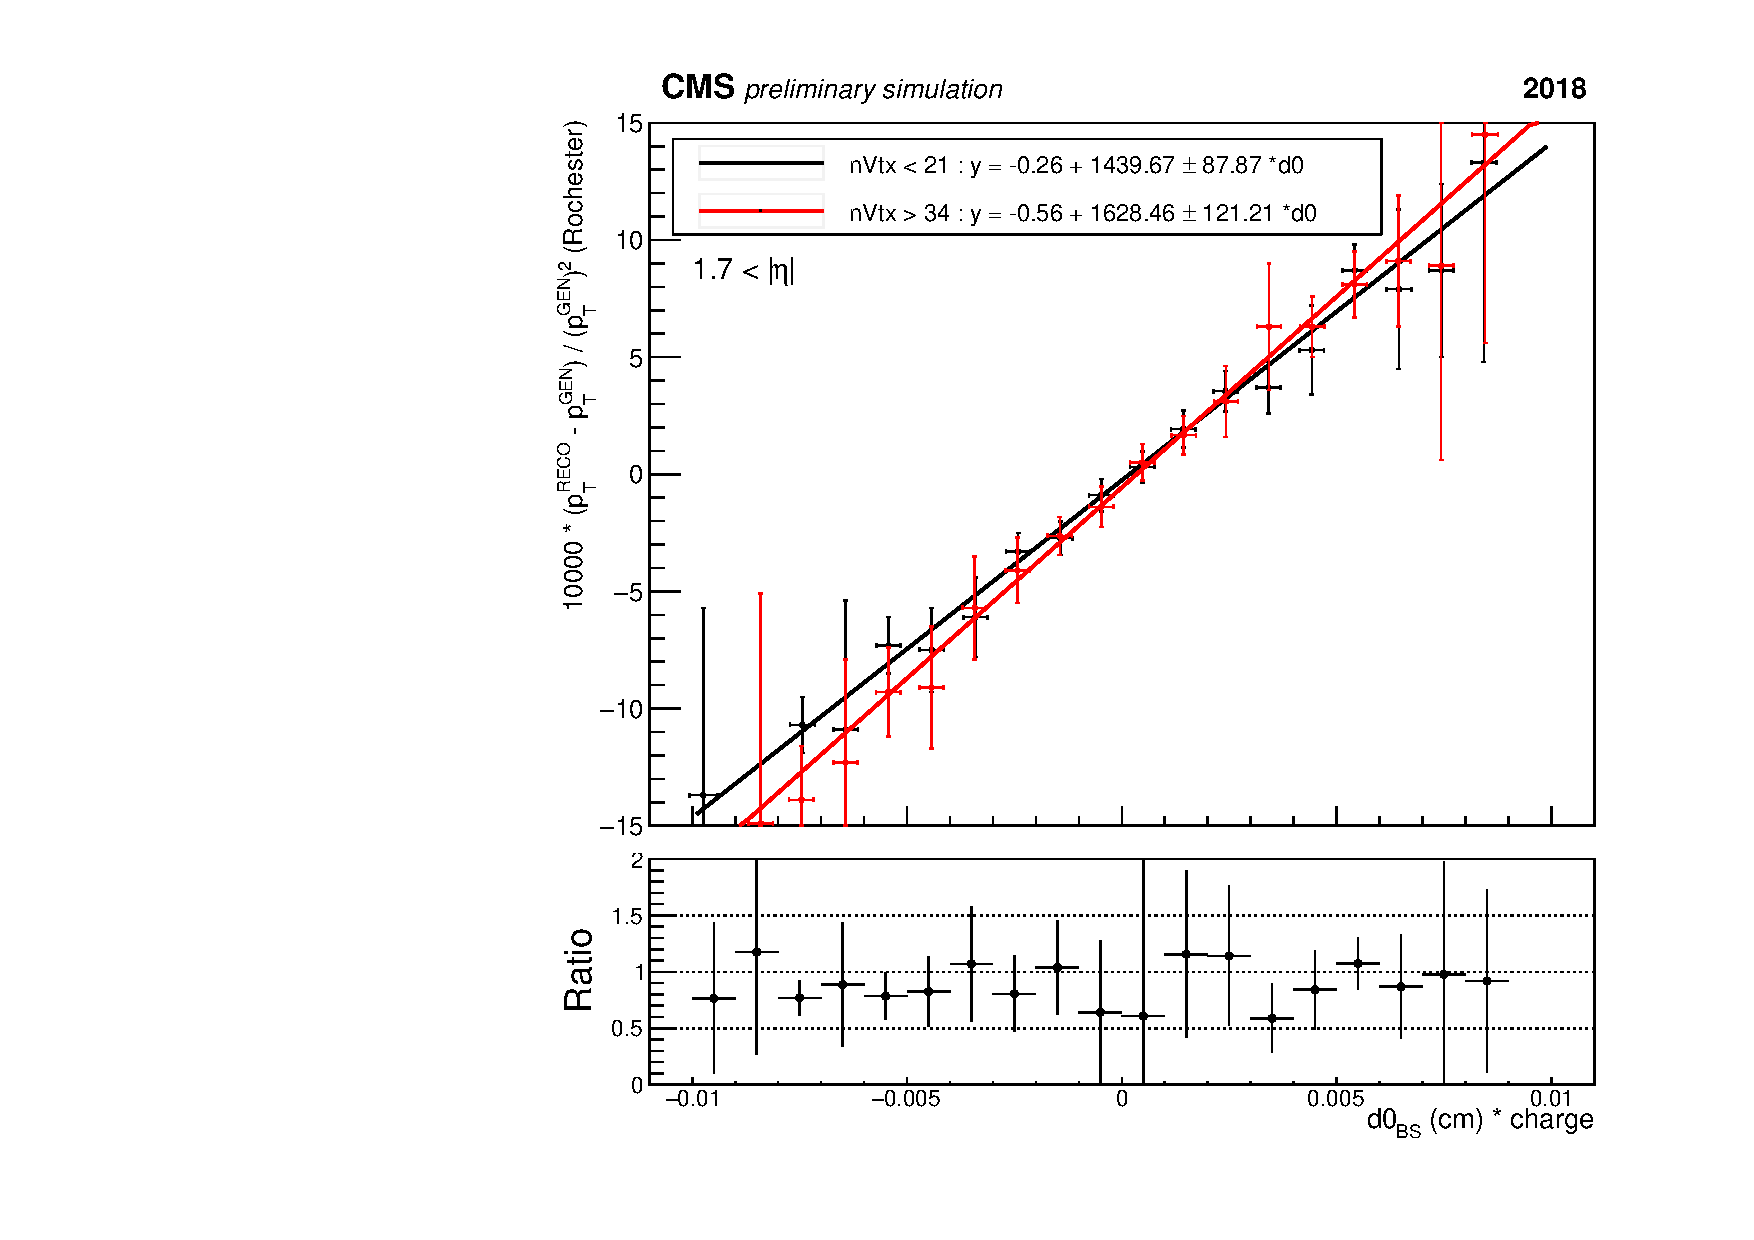
\includegraphics[width=0.32\textwidth]{images_geofit/nVtx_eta_1p7_inf_2018.pdf}
    \caption{Plots comparing \dptoverptsquare vs \dzeroBS distributions for events with number of vertices less than 21 and number of vertices more than 34 for each $|\eta|$ region derived from Z+jets MC in 2018. The ratio plot show the ratio between the black data points (nVtx $<$ 21) and the red data points (nVtx $>$ 34).}
    \label{fig:nVtx_d0_2018}
\end{figure}

Figures~\ref{fig:muCharge_d0_2016},~\ref{fig:muCharge_d0_2017}, and ~\ref{fig:muCharge_d0_2018} show the dependence of \textit{GeoFit Corrections} on muon charge. The constants of proportionality derived by using only $\mu^-$ or $\mu^+$ are consistent with each other. Therefore \textit{GeoFit Corrections} do not depend on the muon charge.

\begin{figure}[h!]
    \centering
    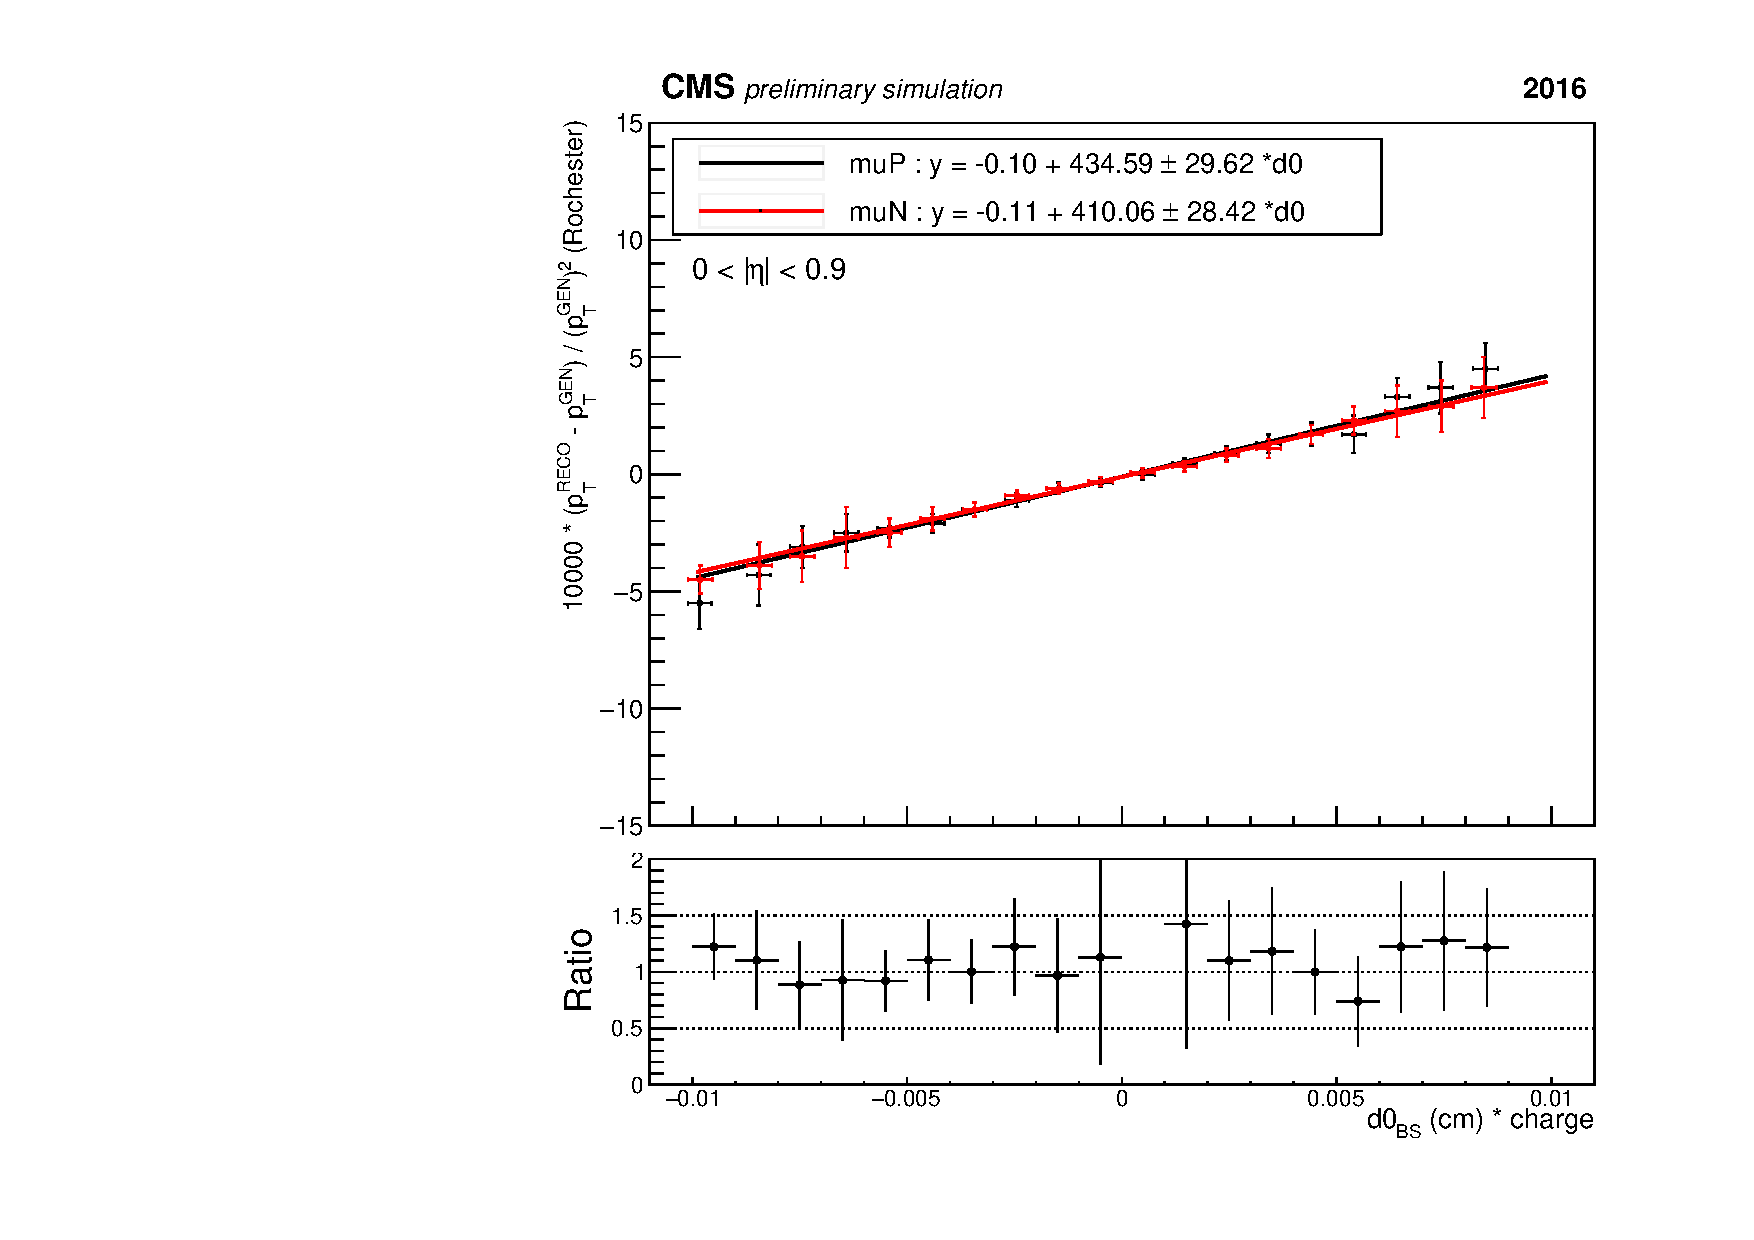
\includegraphics[width=0.32\textwidth]{images_geofit/muCharge_eta_0_0p9_2016.pdf}
    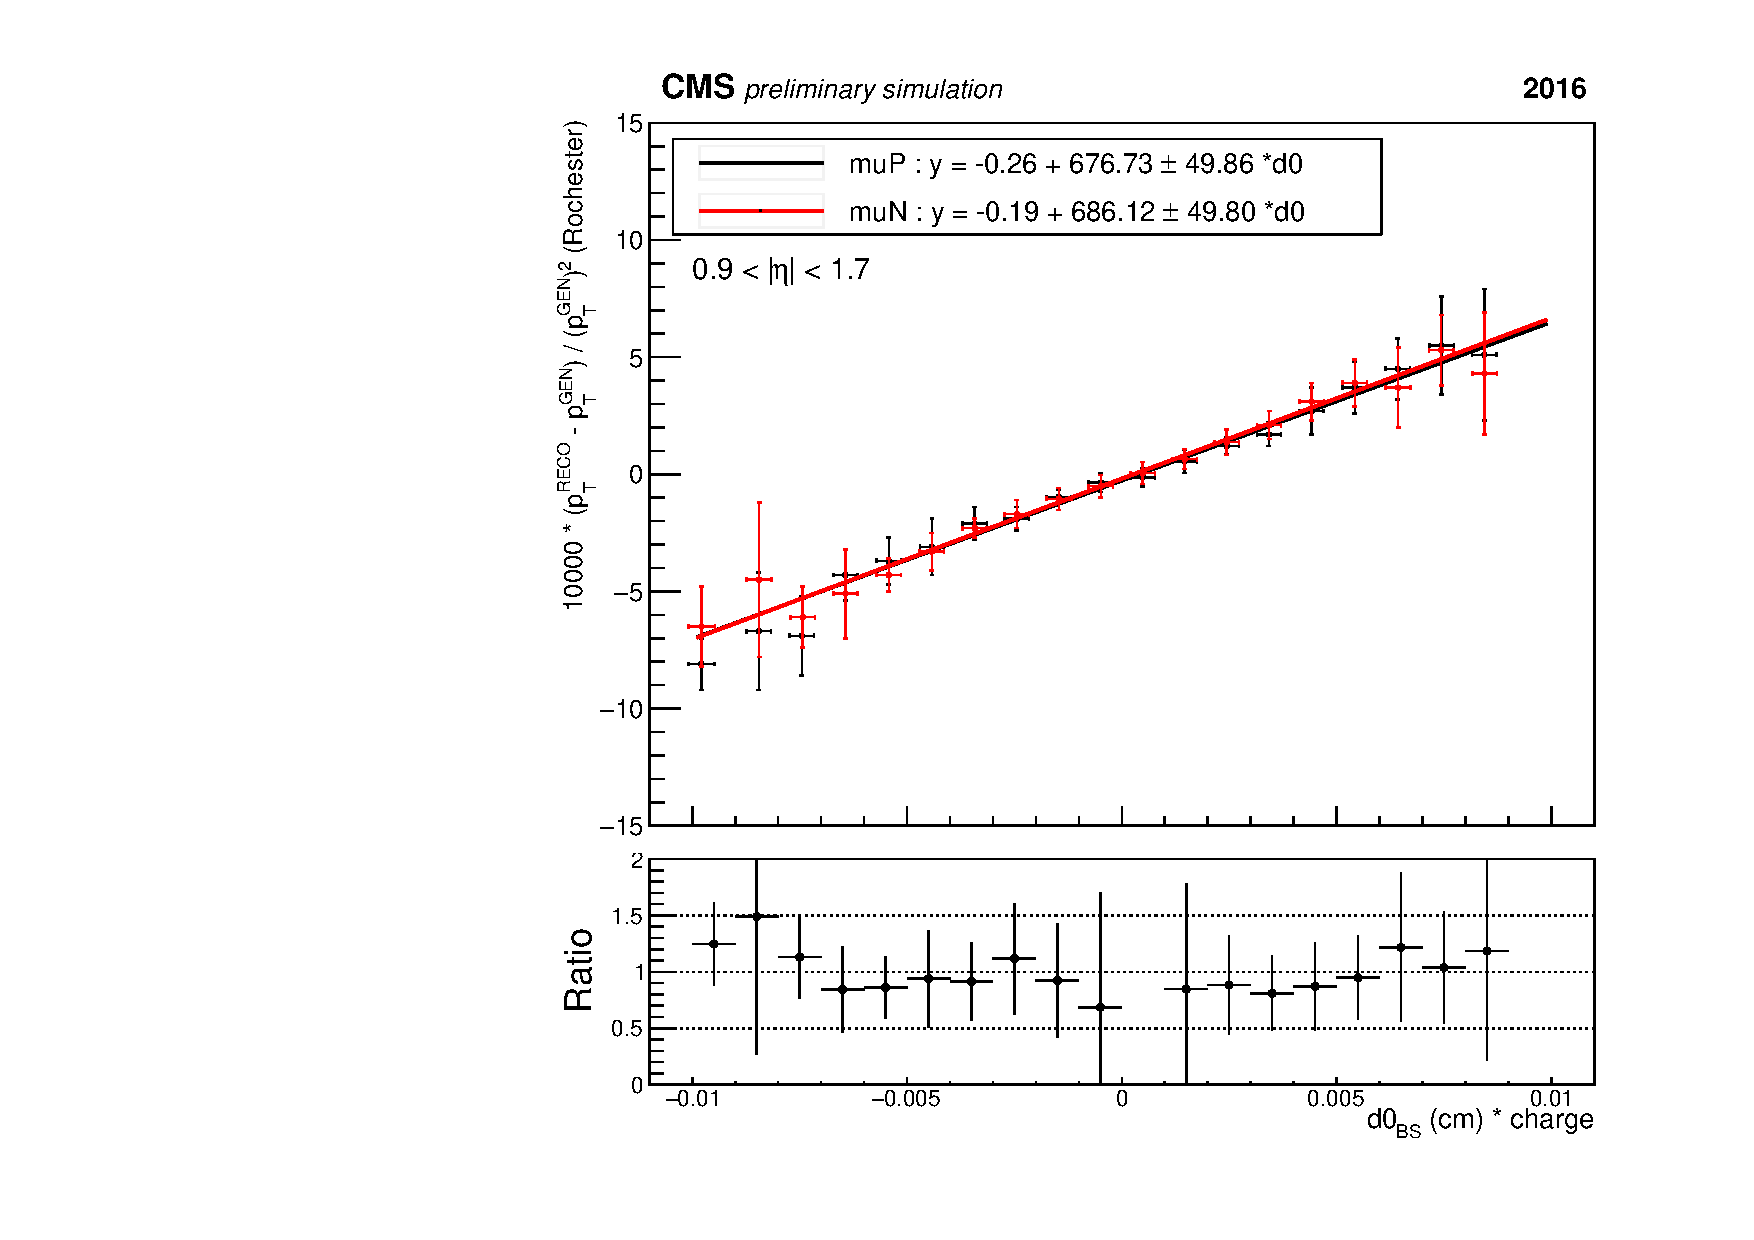
\includegraphics[width=0.32\textwidth]{images_geofit/muCharge_eta_0p9_1p7_2016.pdf}
    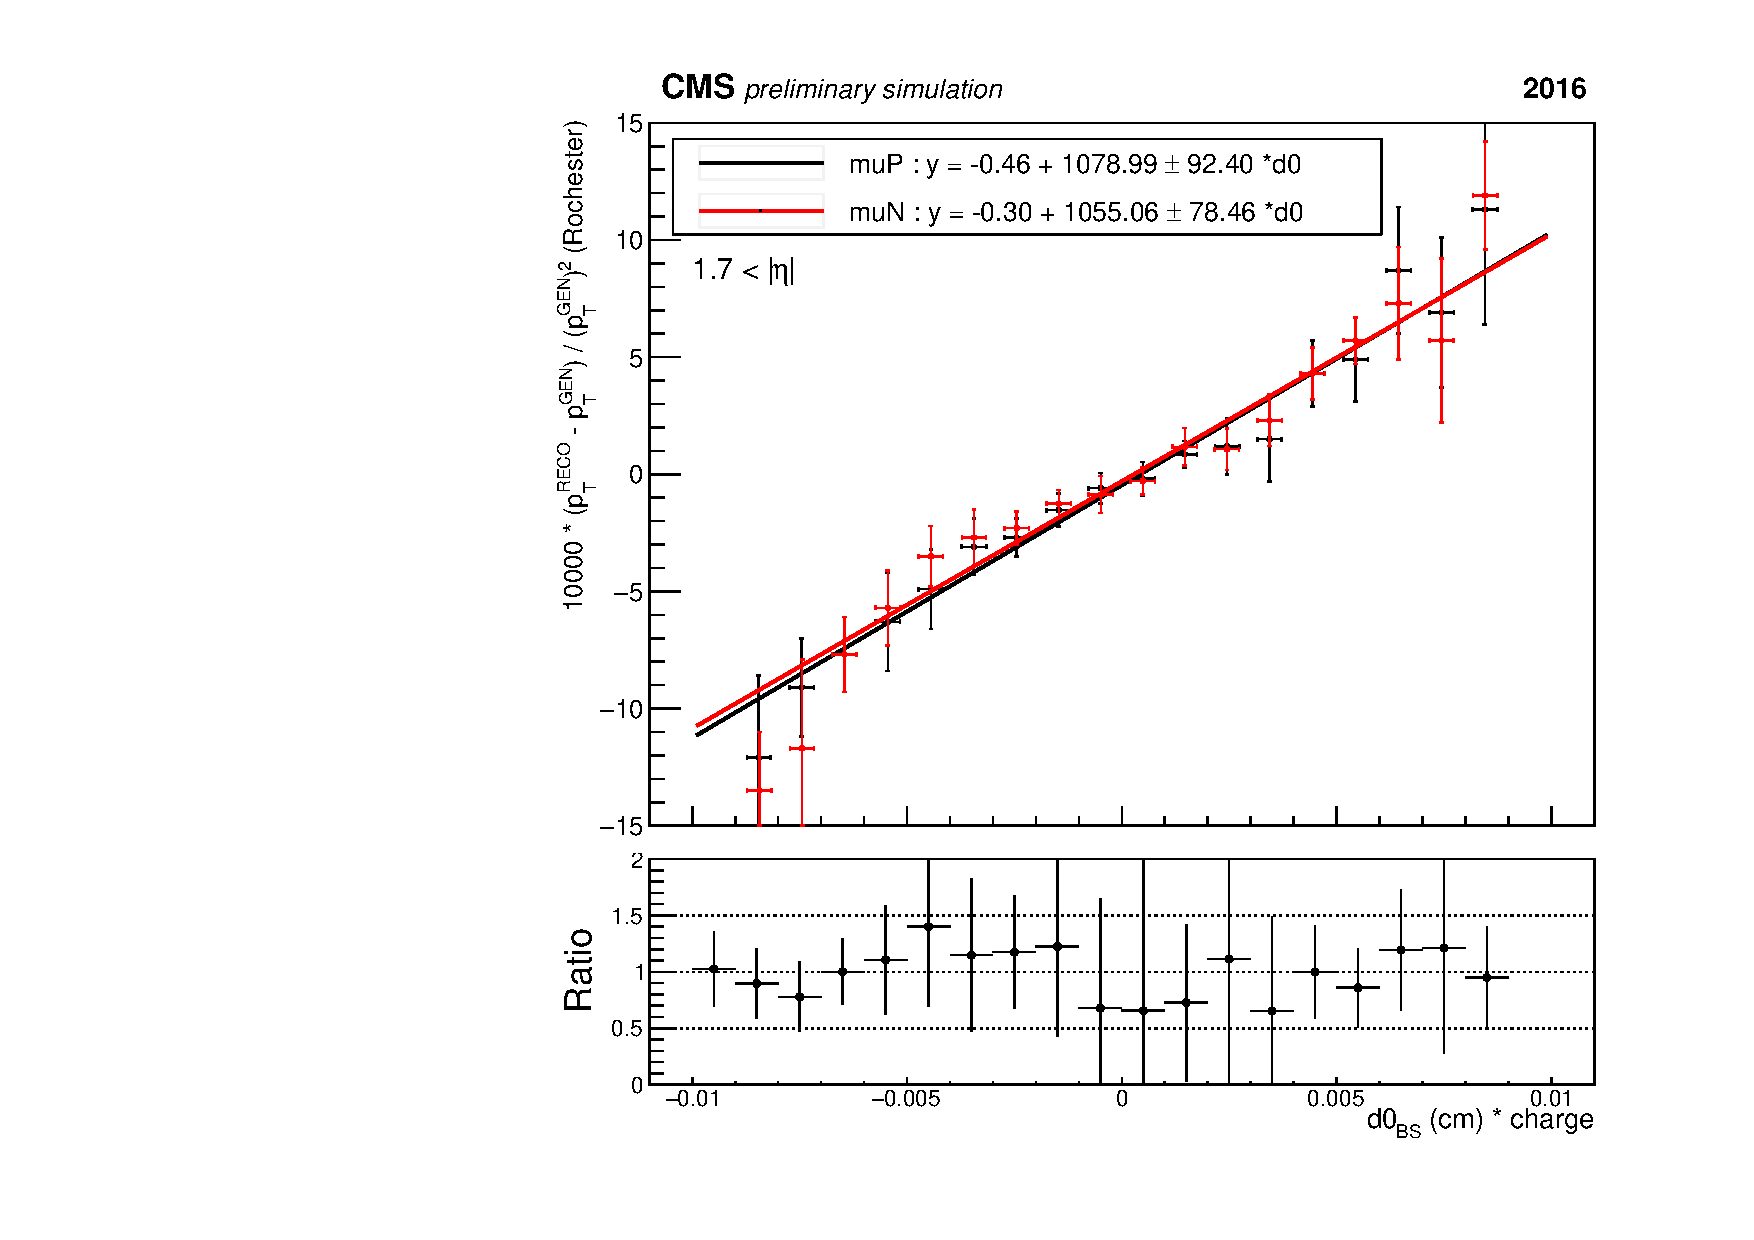
\includegraphics[width=0.32\textwidth]{images_geofit/muCharge_eta_1p7_inf_2016.pdf}
    \caption{Plots comparing \dptoverptsquare vs \dzeroBS distributions for $\mu^+$ and $\mu^-$ for each $|\eta|$ region derived from Z+jets MC in 2016. The ratio plot show the ratio between the black data points ($\mu^+$) and the red data points ($\mu^-$).}
    \label{fig:muCharge_d0_2016}
\end{figure}

\begin{figure}[h!]
    \centering
    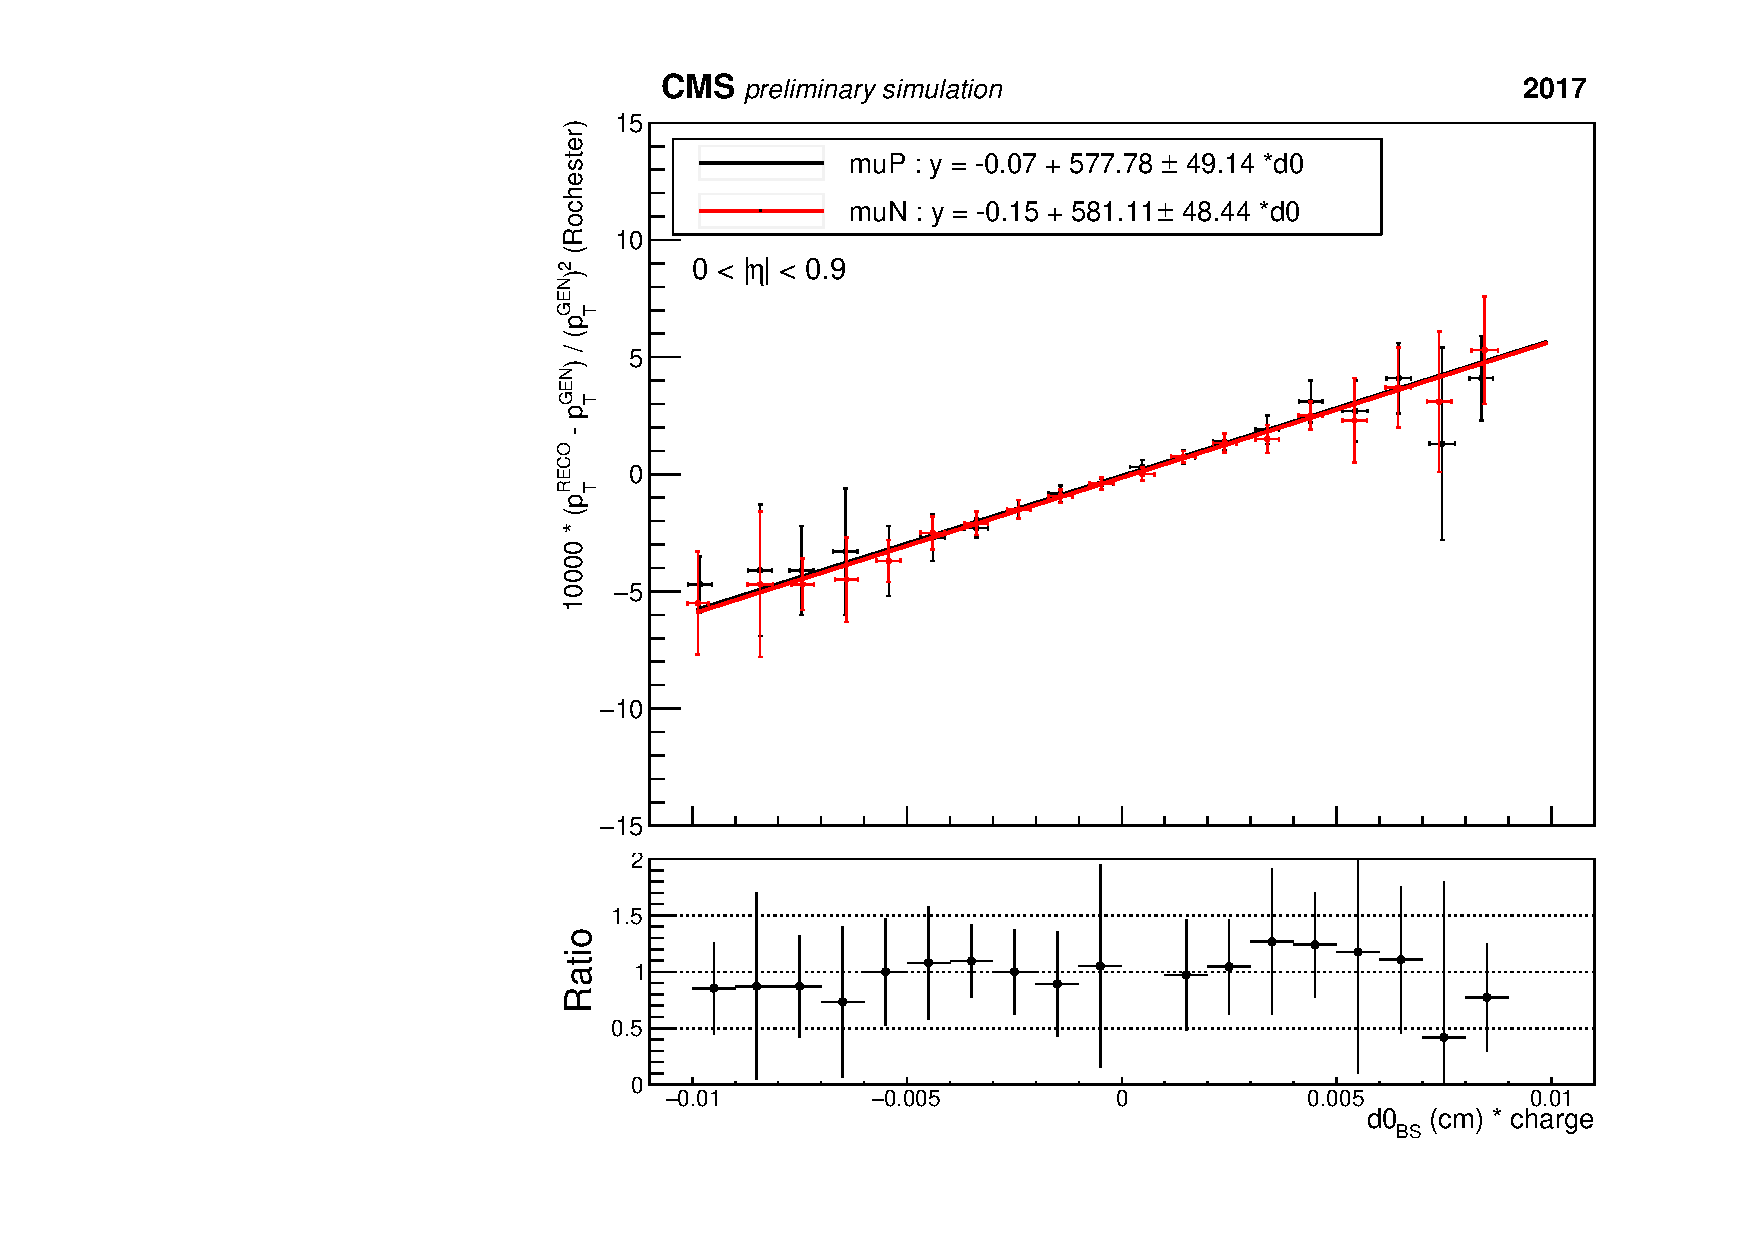
\includegraphics[width=0.32\textwidth]{images_geofit/muCharge_eta_0_0p9_2017.pdf}
    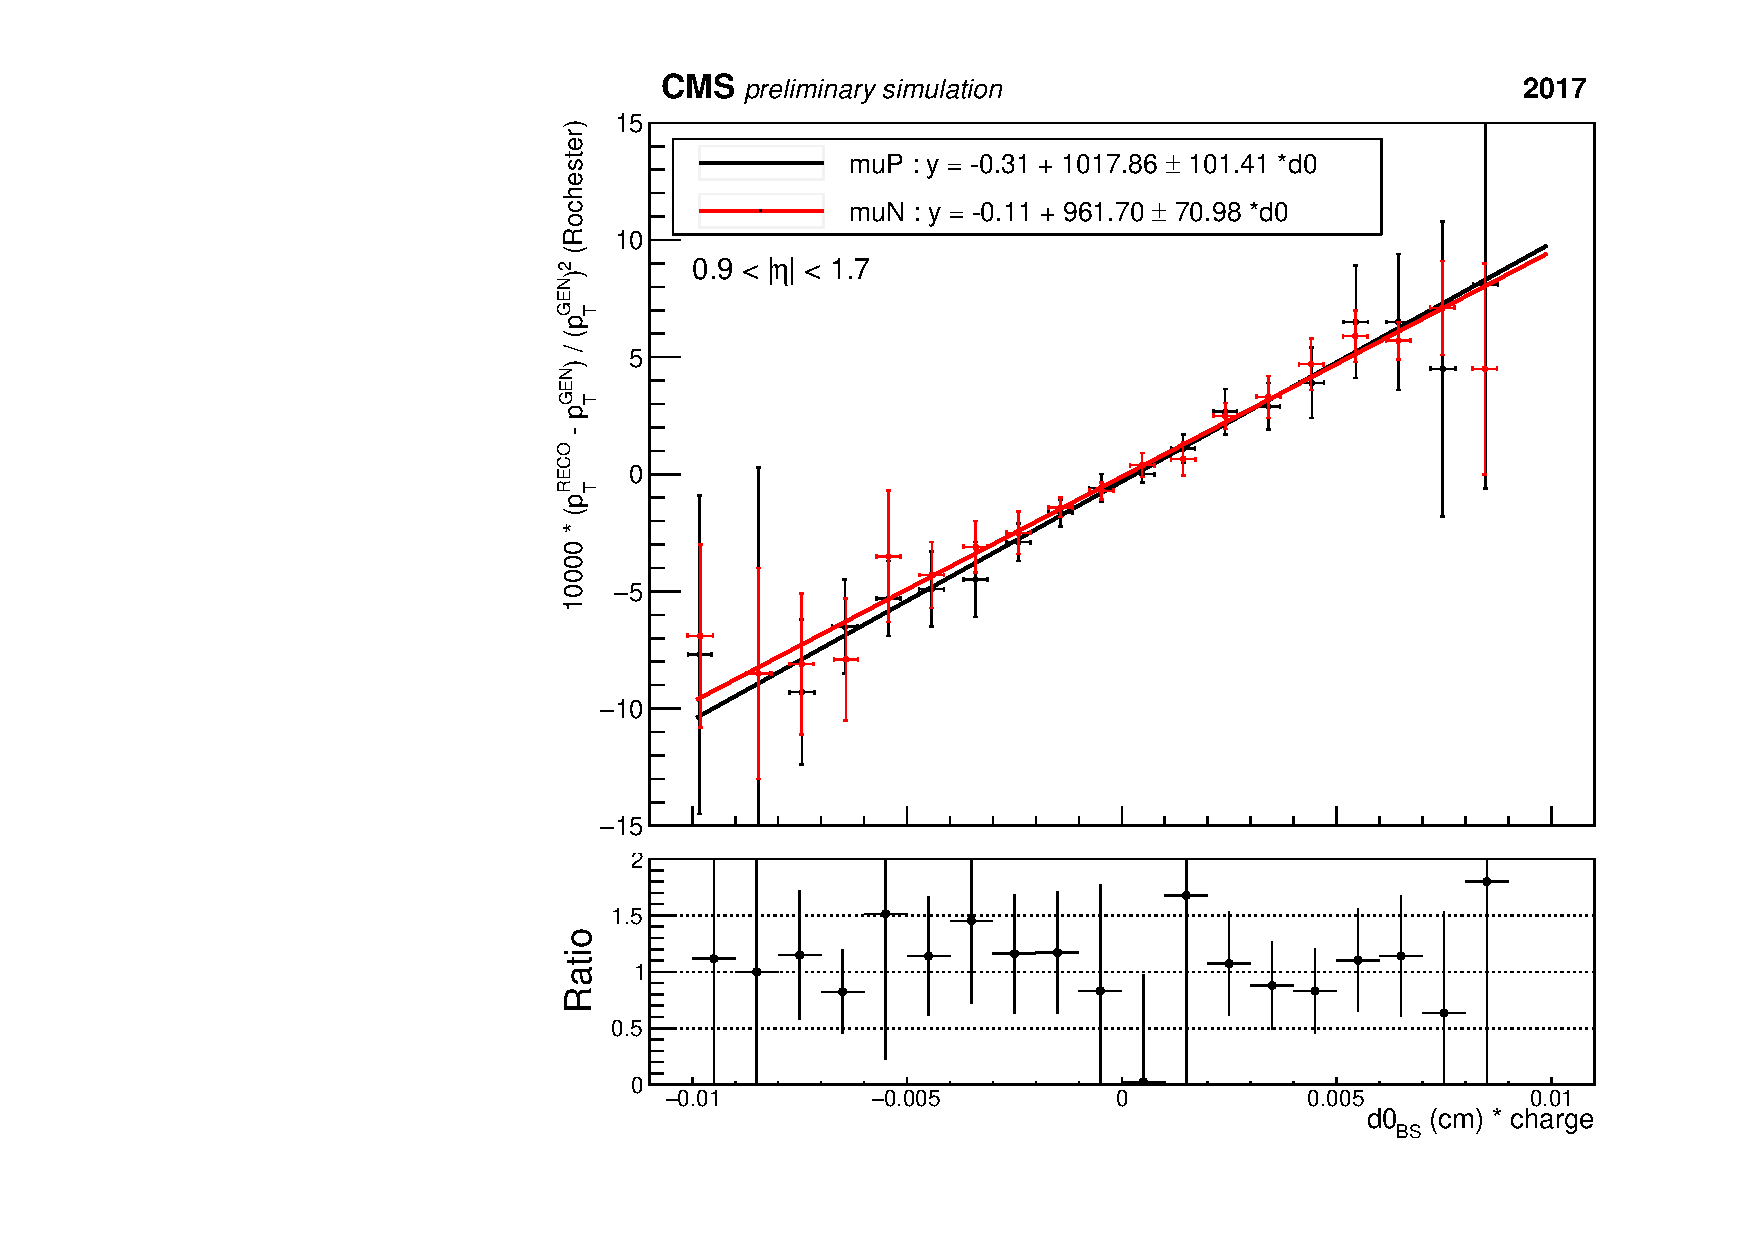
\includegraphics[width=0.32\textwidth]{images_geofit/muCharge_eta_0p9_1p7_2017.pdf}
    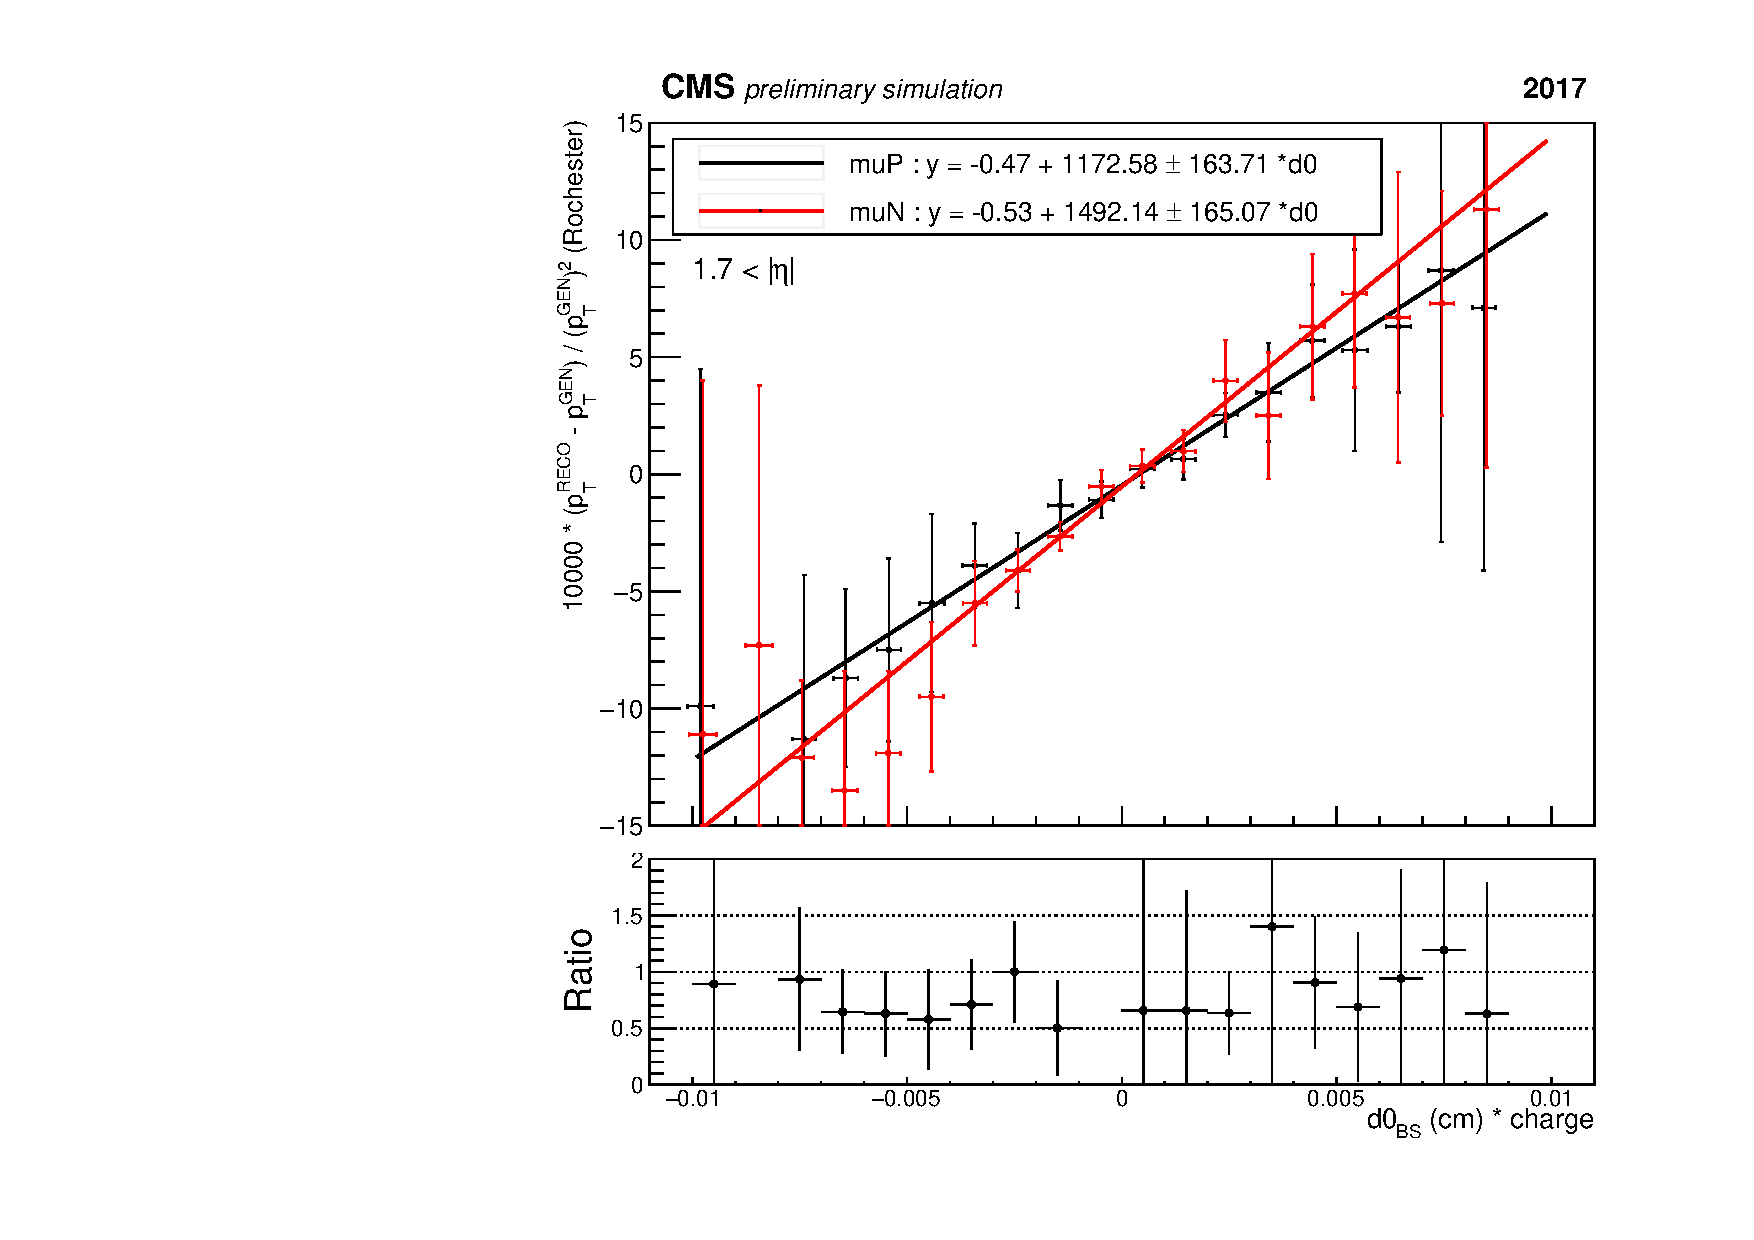
\includegraphics[width=0.32\textwidth]{images_geofit/muCharge_eta_1p7_inf_2017.pdf}
    \caption{Plots comparing \dptoverptsquare vs \dzeroBS distributions for $\mu^+$ and $\mu^-$ for each $|\eta|$ region derived from Z+jets MC in 2017. The ratio plot show the ratio between the black data points ($\mu^+$) and the red data points ($\mu^-$).}
    \label{fig:muCharge_d0_2017}
\end{figure}

\begin{figure}[h!]
    \centering
    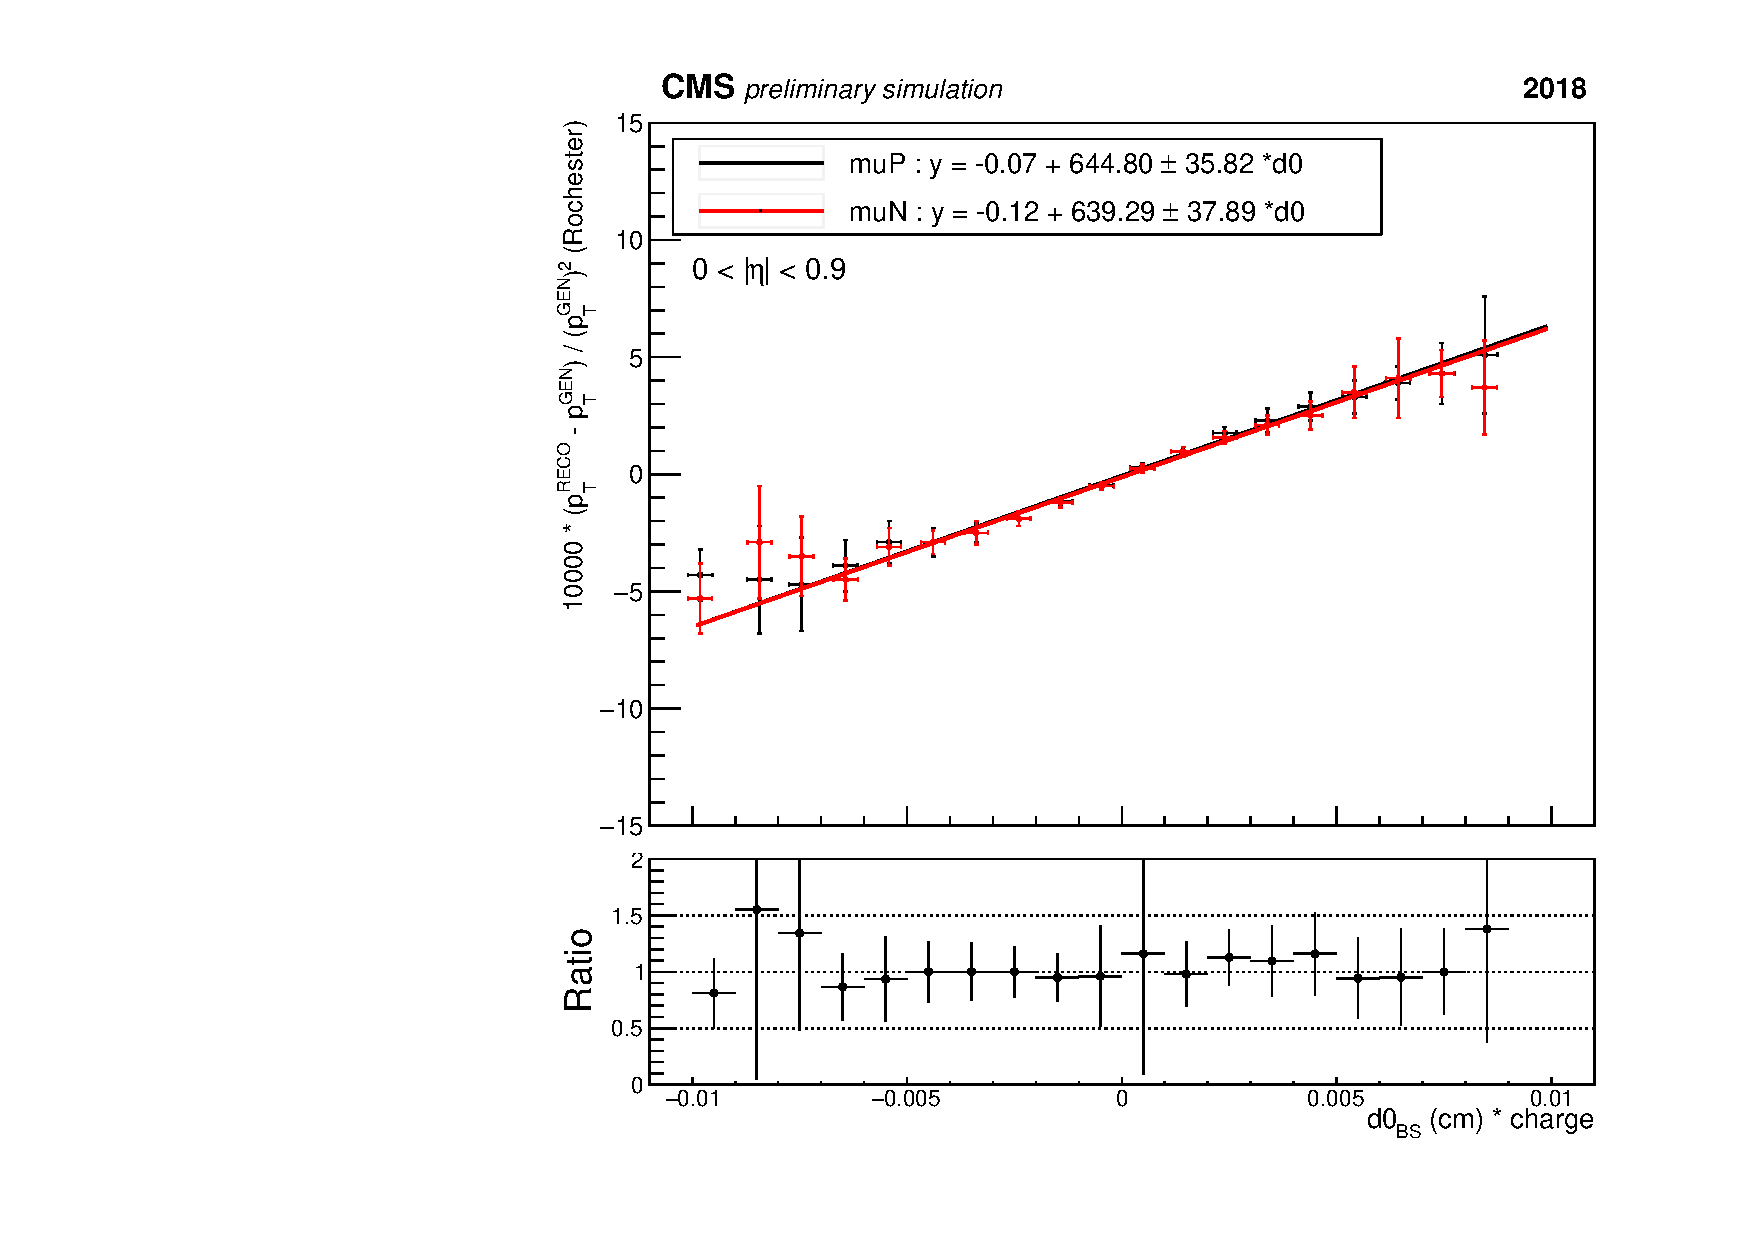
\includegraphics[width=0.32\textwidth]{images_geofit/muCharge_eta_0_0p9_2018.pdf}
    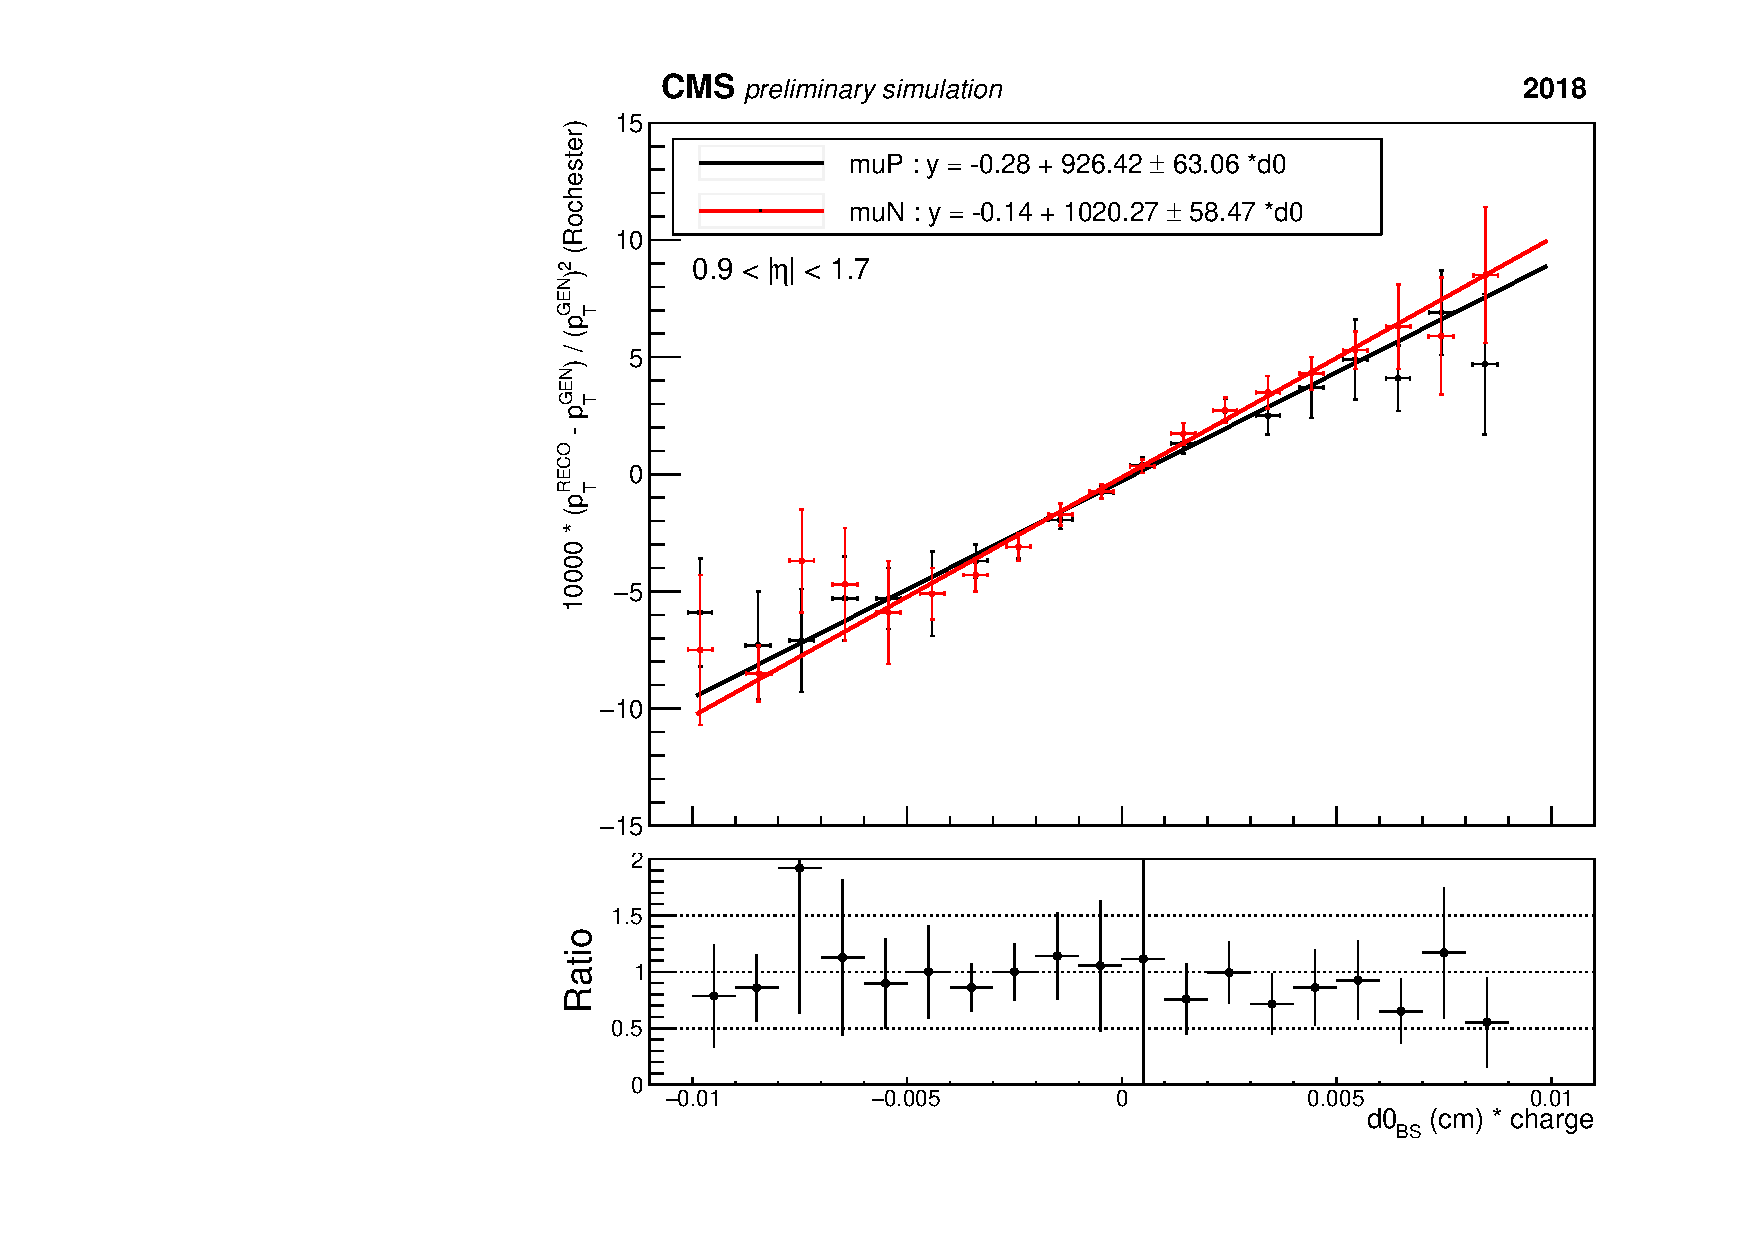
\includegraphics[width=0.32\textwidth]{images_geofit/muCharge_eta_0p9_1p7_2018.pdf}
    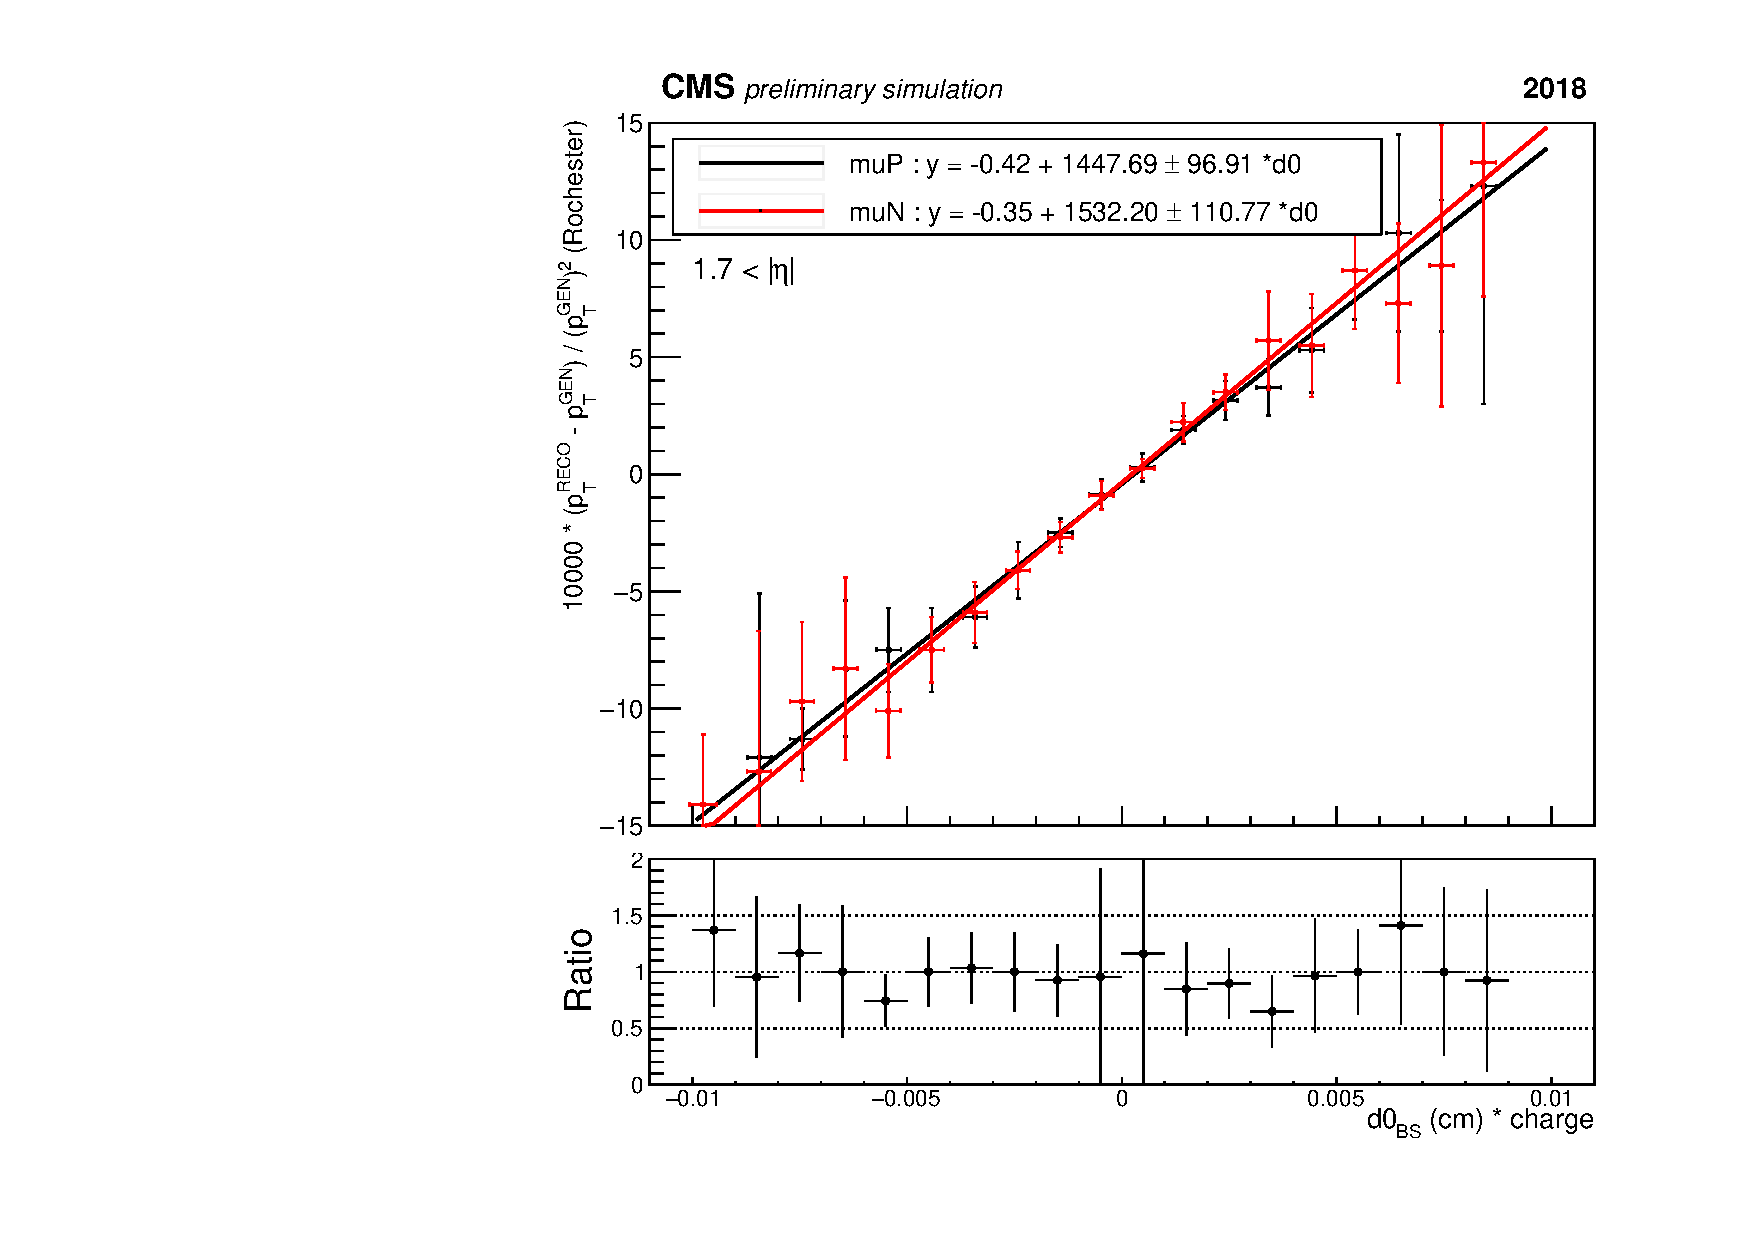
\includegraphics[width=0.32\textwidth]{images_geofit/muCharge_eta_1p7_inf_2018.pdf}
    \caption{Plots comparing \dptoverptsquare vs \dzeroBS distributions for $\mu^+$ and $\mu^-$ for each $|\eta|$ region derived from Z+jets MC in 2018. The ratio plot show the ratio between the black data points ($\mu^+$) and the red data points ($\mu^-$).}
    \label{fig:muCharge_d0_2018}
\end{figure}

Figures~\ref{fig:ttH_d0_2016},~\ref{fig:ttH_d0_2017}, and ~\ref{fig:ttH_d0_2018} show the dependence of \textit{GeoFit Corrections} on number of tracks in the vertex. This is achieved by considering ttH MC samples instead of Z+jets MC samples due to ttH samples having more high \pt prompt objects in the event. The constants of proportionality derived from each sample is consistent with each other, which shows that the \textit{GeoFit Corrections} do not depend strongly on the number of tracks in the vertex.

\begin{figure}[h!]
    \centering
    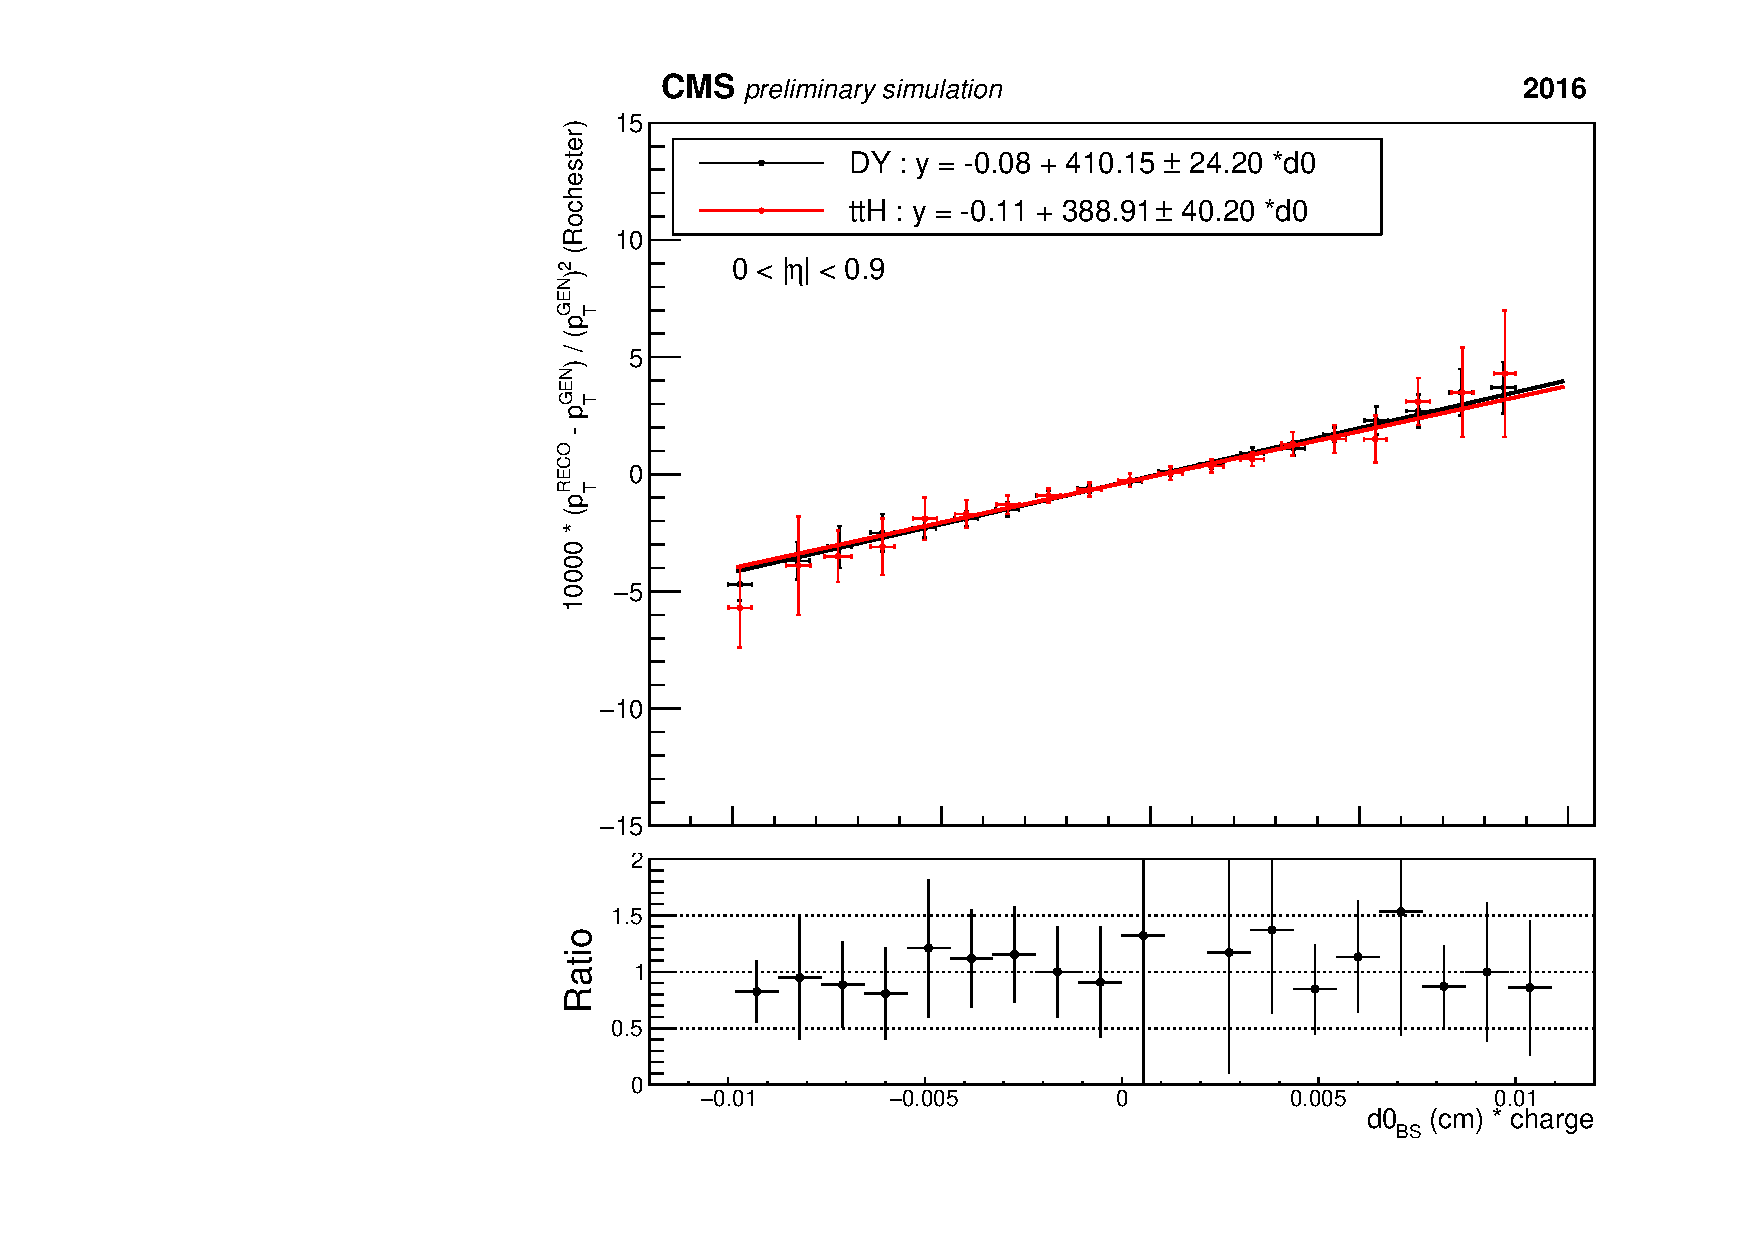
\includegraphics[width=0.32\textwidth]{images_geofit/ttH_eta_0_0p9_2016.pdf}
    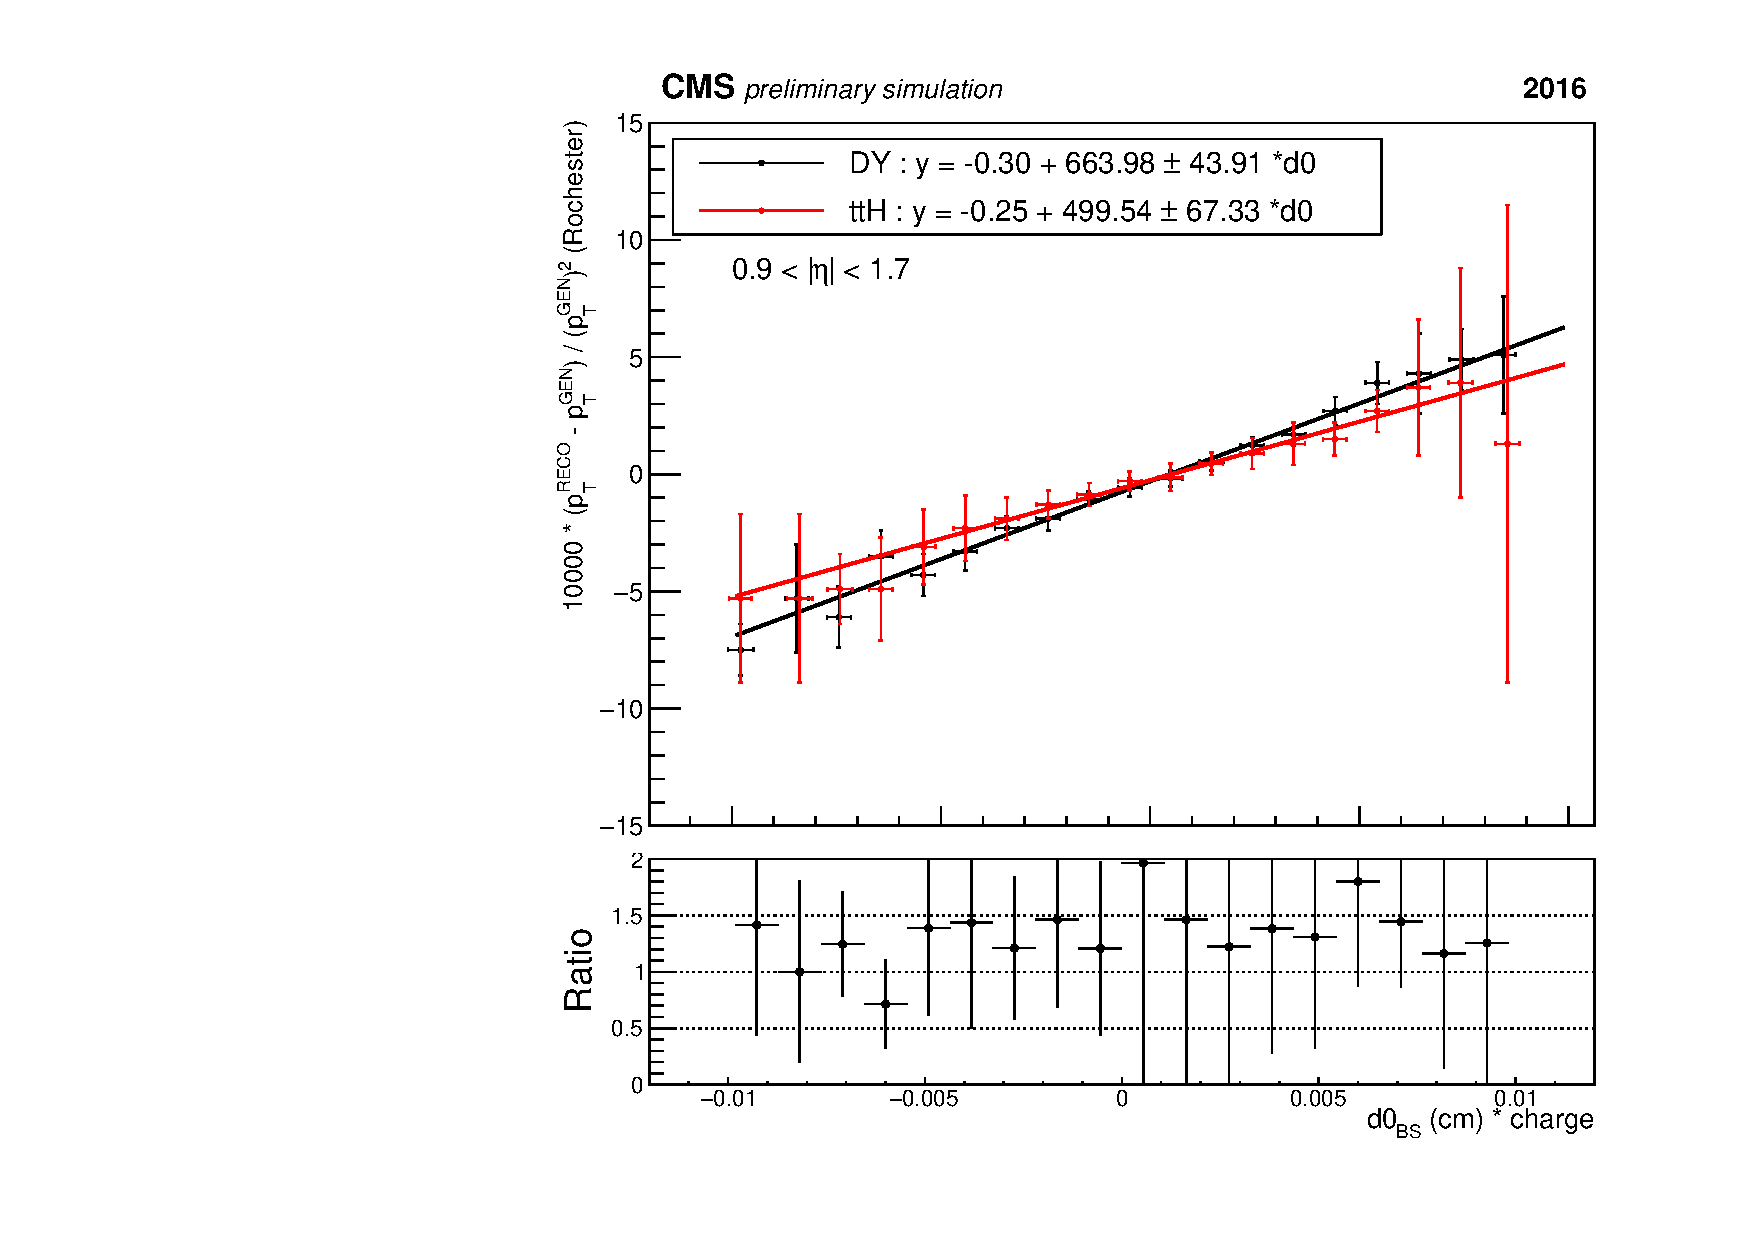
\includegraphics[width=0.32\textwidth]{images_geofit/ttH_eta_0p9_1p7_2016.pdf}
    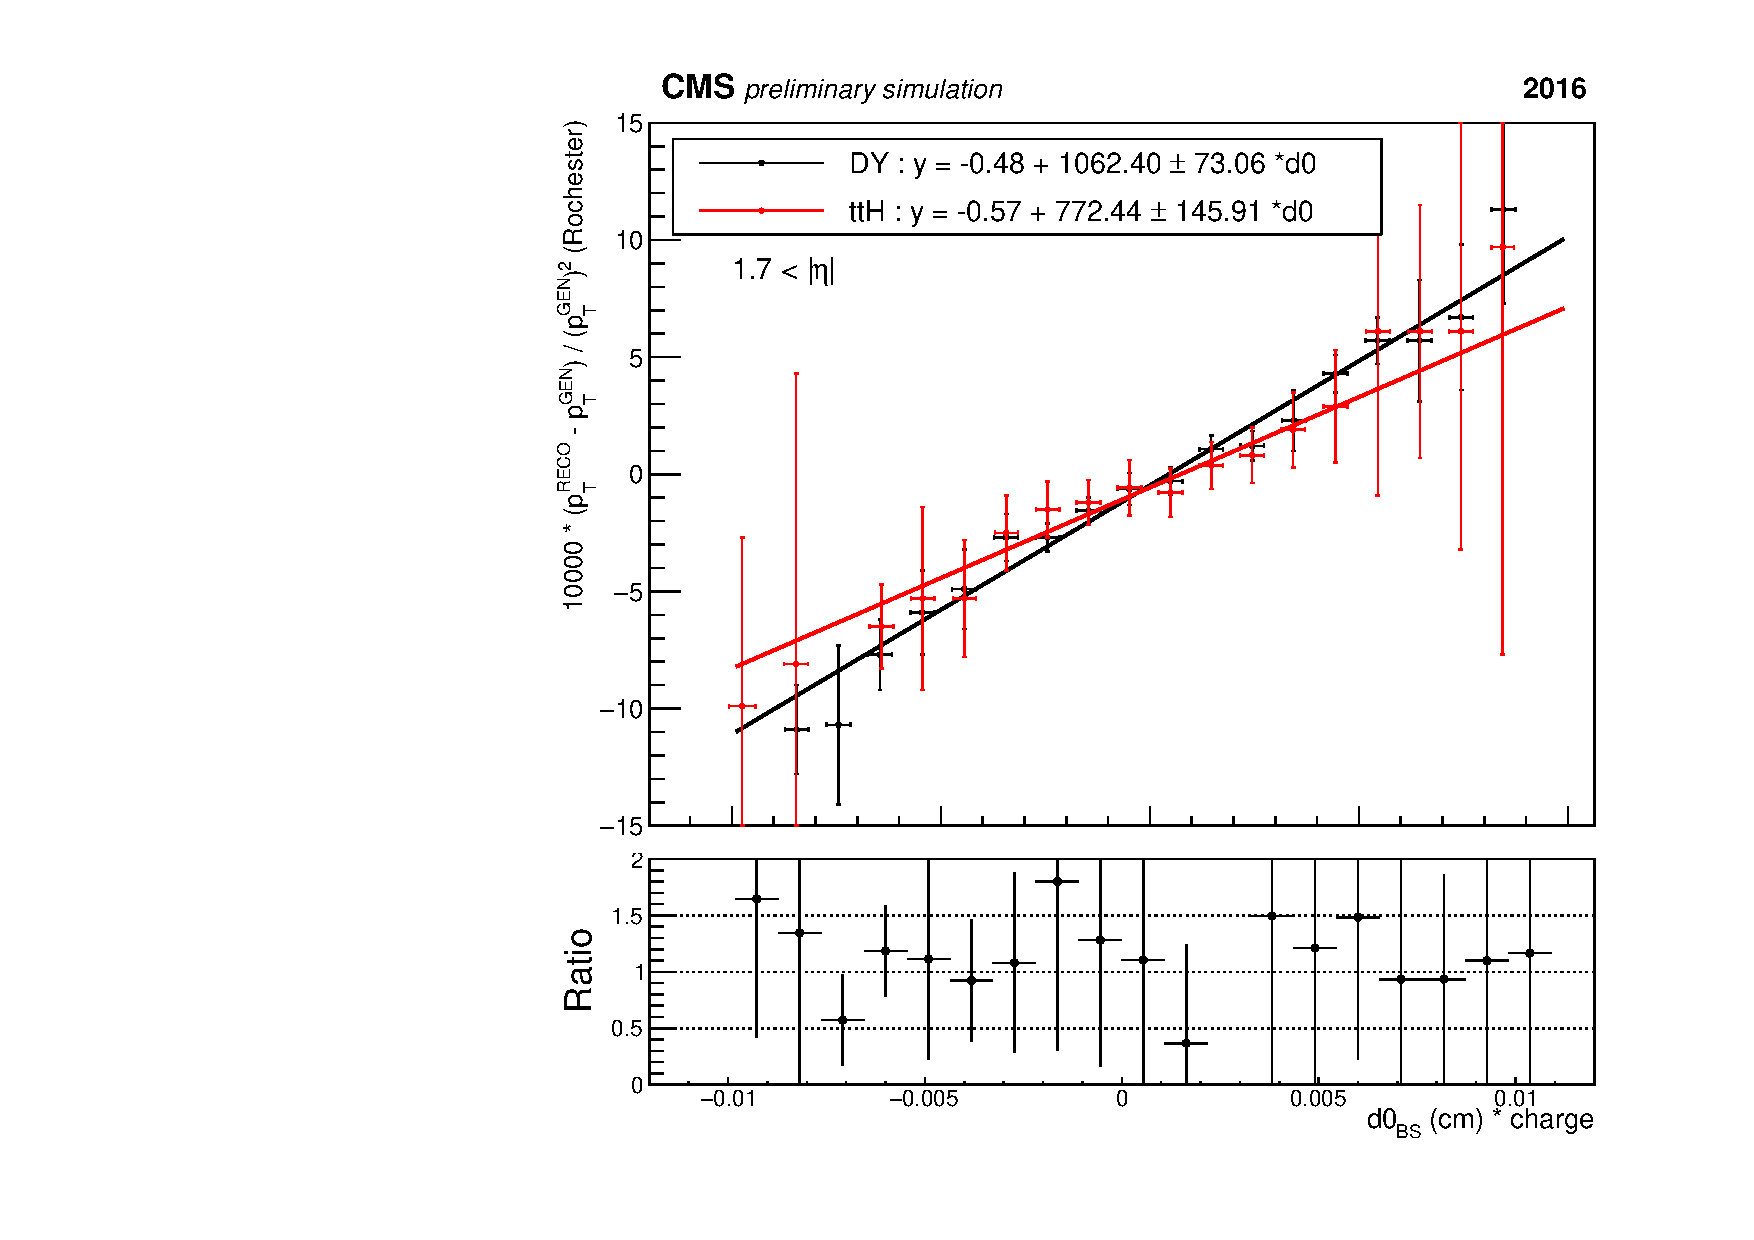
\includegraphics[width=0.32\textwidth]{images_geofit/ttH_eta_1p7_inf_2016.pdf}
    \caption{Plots comparing \dptoverptsquare vs \dzeroBS distributions in each $|\eta|$ region derived from Z+jets MC and ttH MC in 2016. The ratio plot show the ratio between the black data points (Z+jets MC) and the red data points (ttH MC).}
    \label{fig:ttH_d0_2016}
\end{figure}

\begin{figure}[h!]
    \centering
    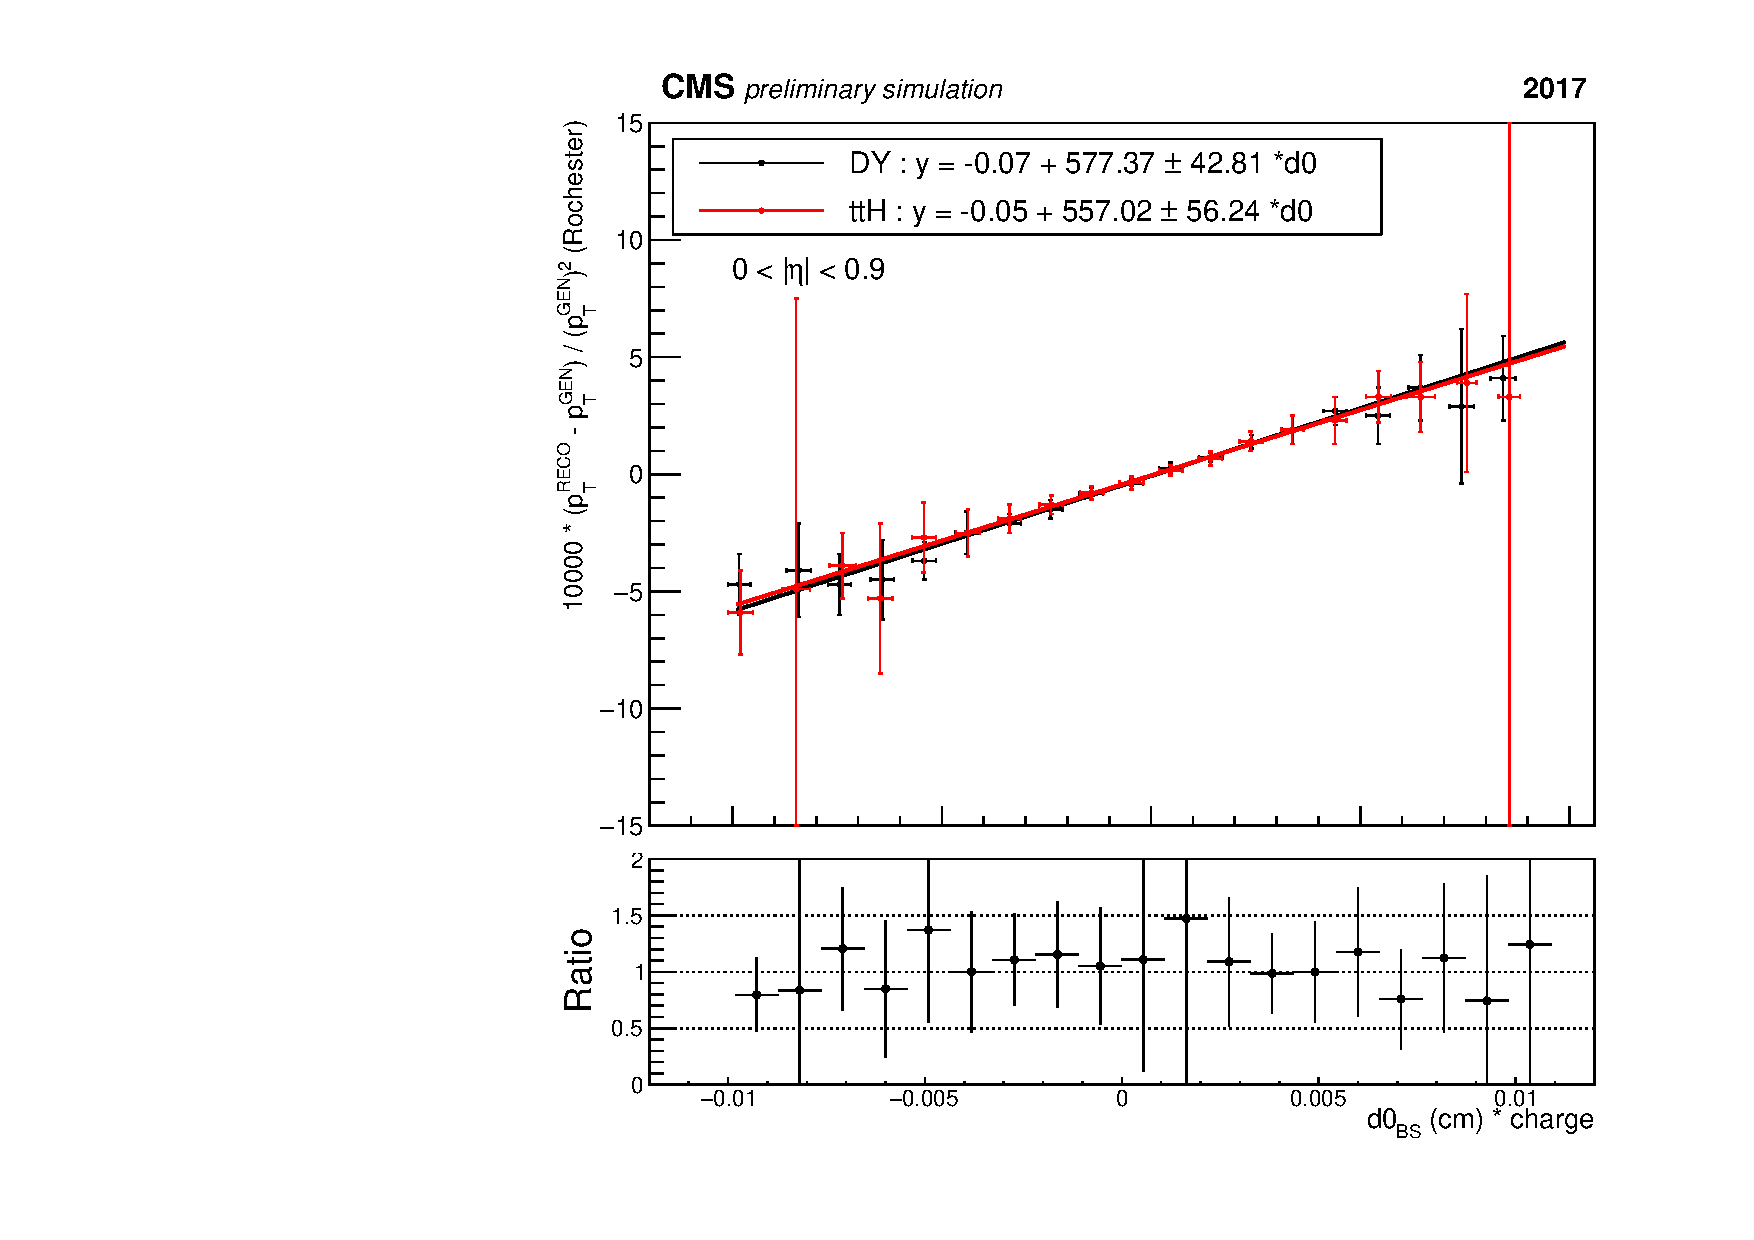
\includegraphics[width=0.32\textwidth]{images_geofit/ttH_eta_0_0p9_2017.pdf}
    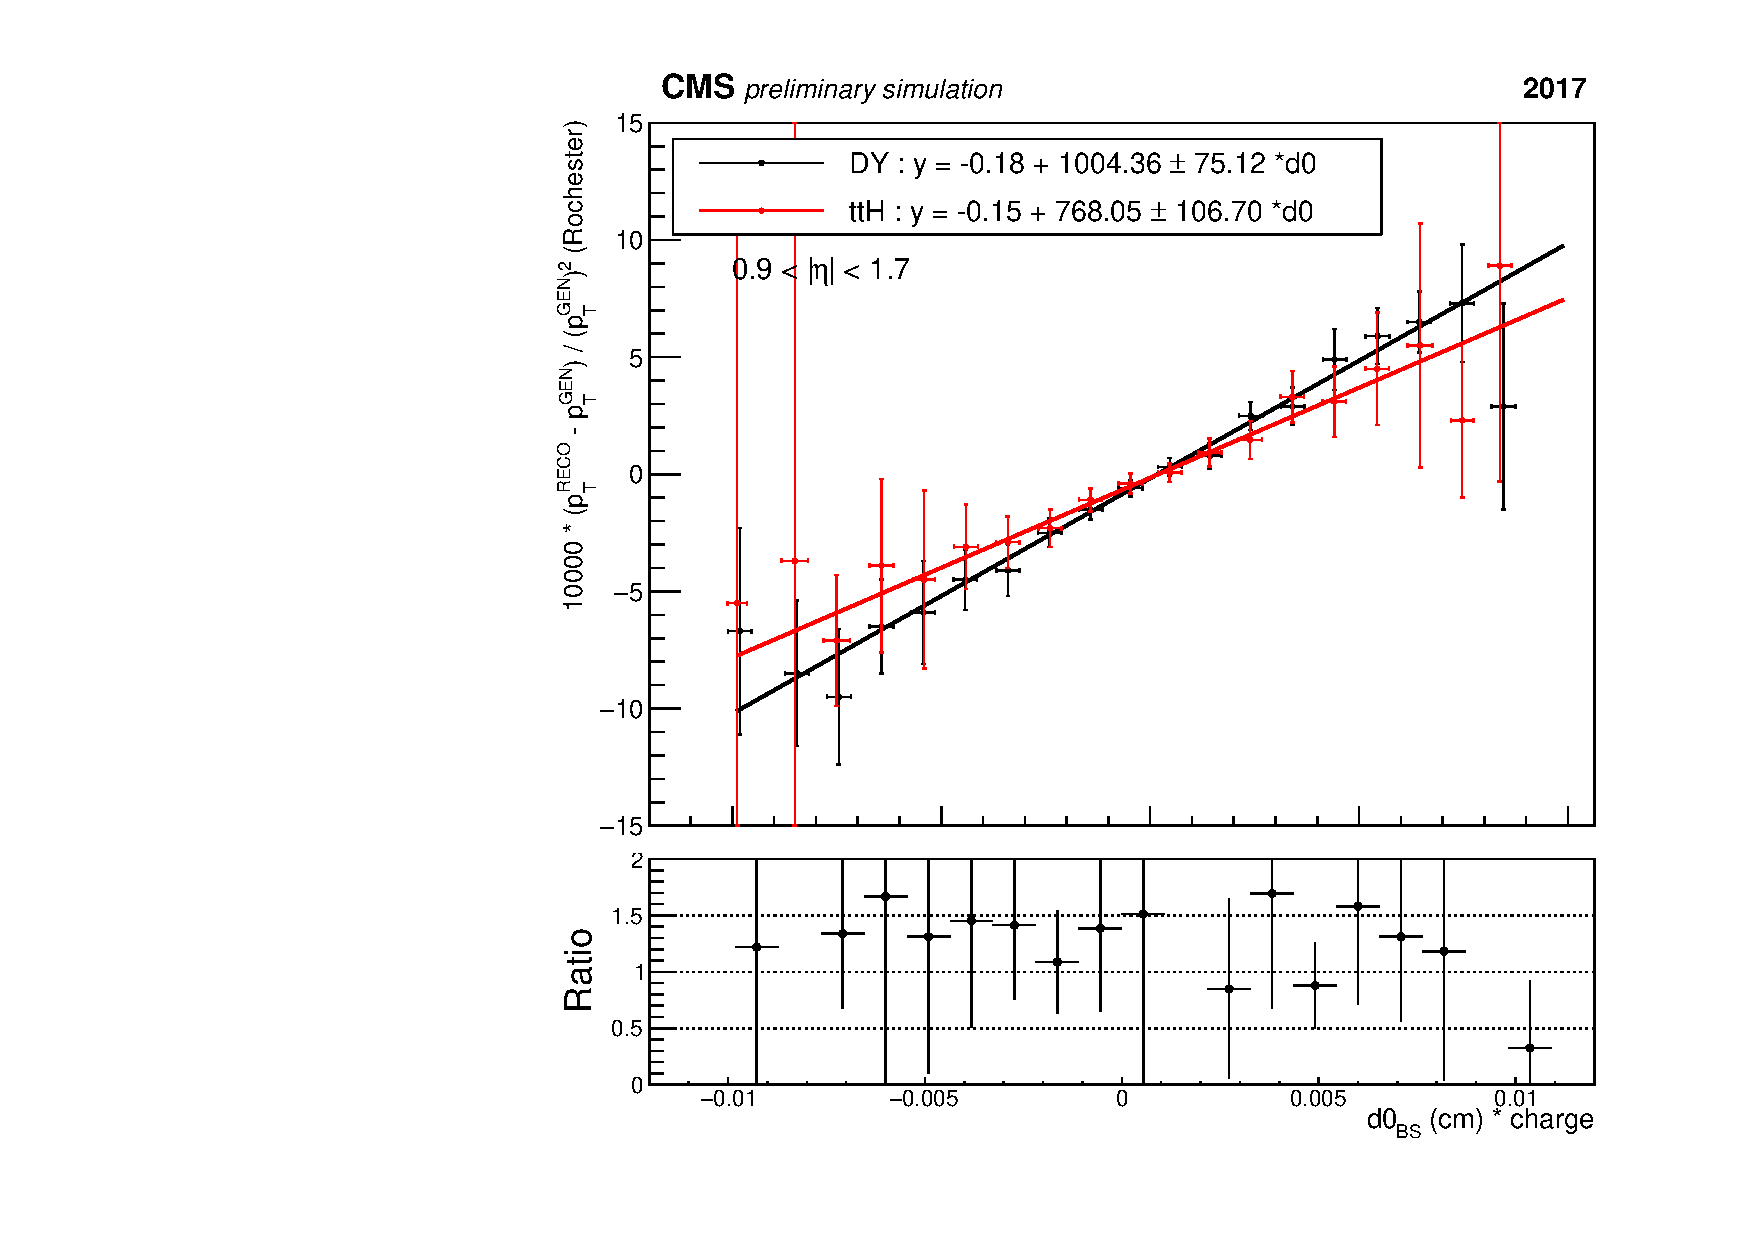
\includegraphics[width=0.32\textwidth]{images_geofit/ttH_eta_0p9_1p7_2017.pdf}
    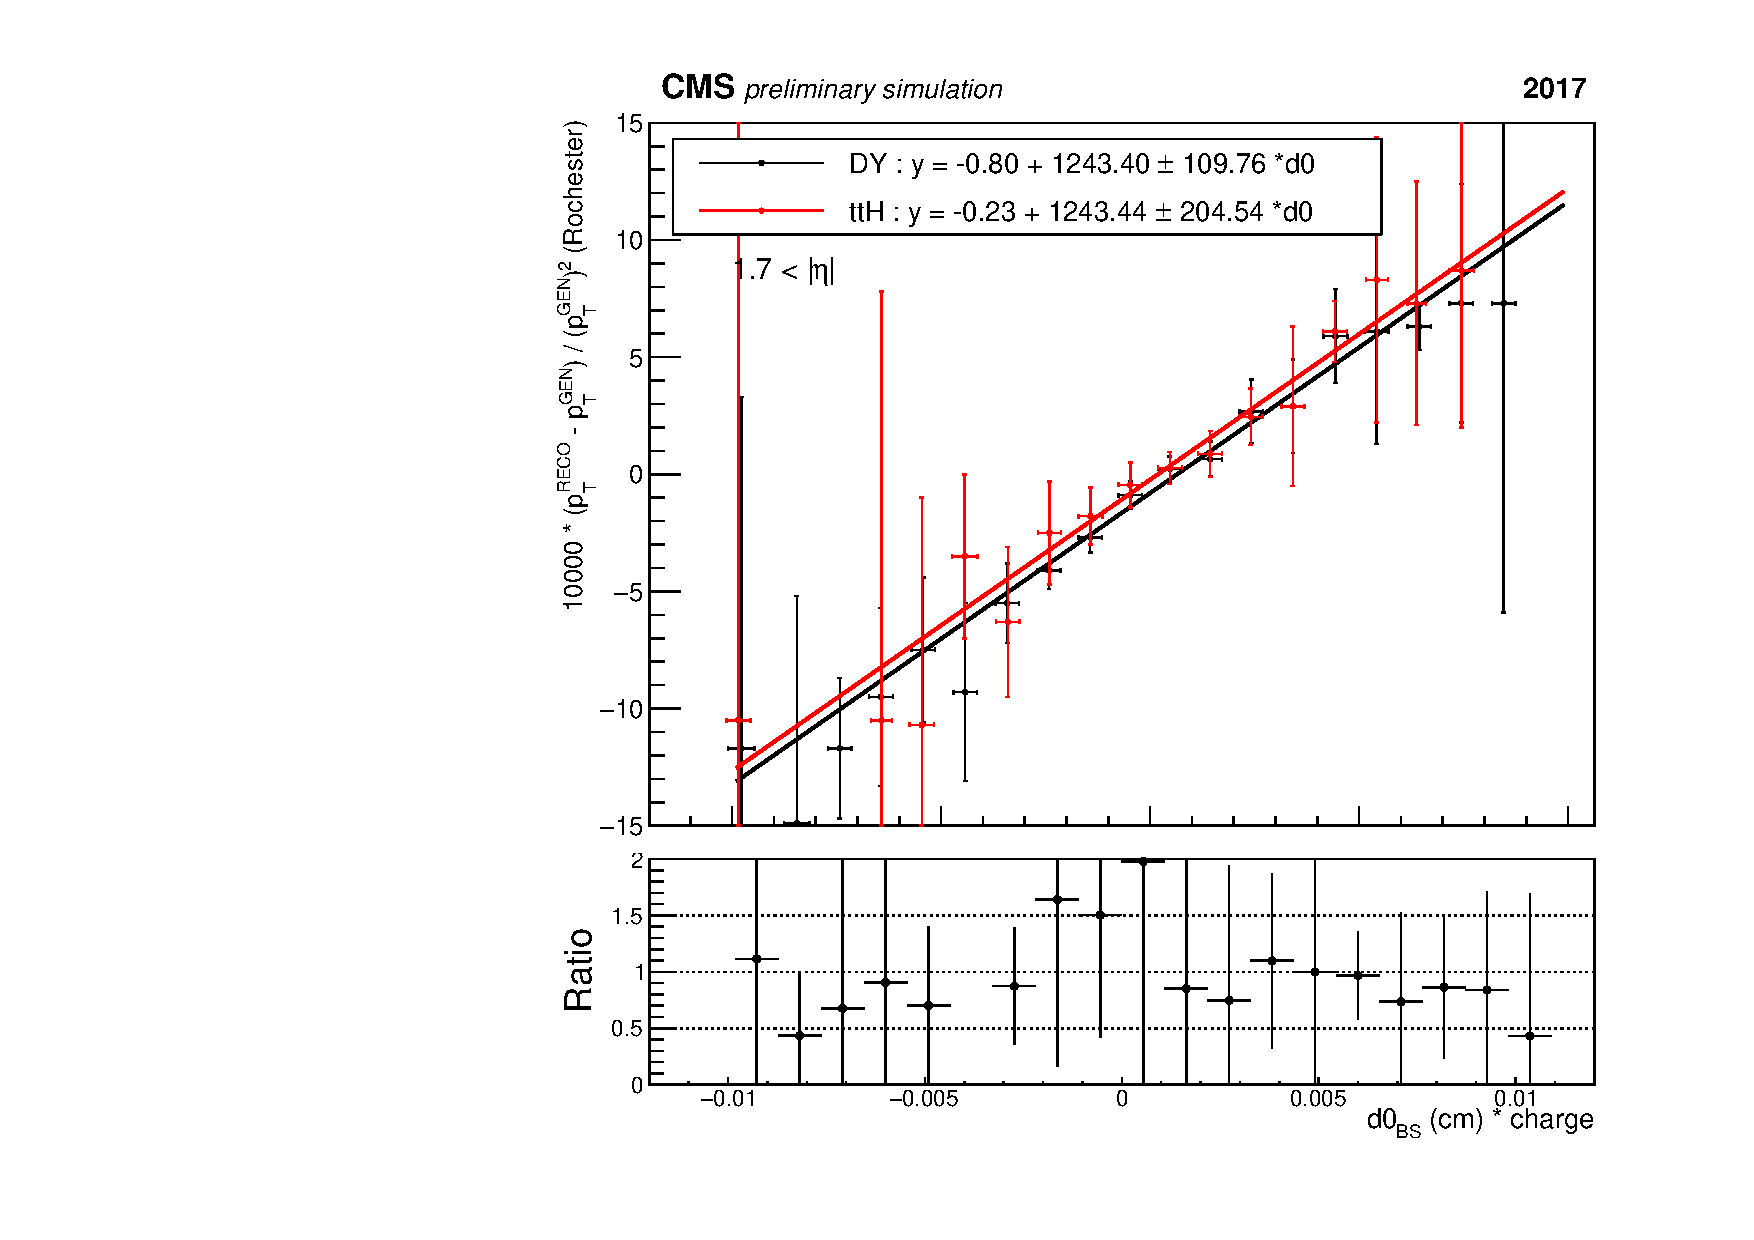
\includegraphics[width=0.32\textwidth]{images_geofit/ttH_eta_1p7_inf_2017.pdf}
    \caption{Plots comparing \dptoverptsquare vs \dzeroBS distributions in each $|\eta|$ region derived from Z+jets MC and ttH MC in 2017. The ratio plot show the ratio between the black data points (Z+jets MC) and the red data points (ttH MC).}
    \label{fig:ttH_d0_2017}
\end{figure}

\begin{figure}[h!]
    \centering
    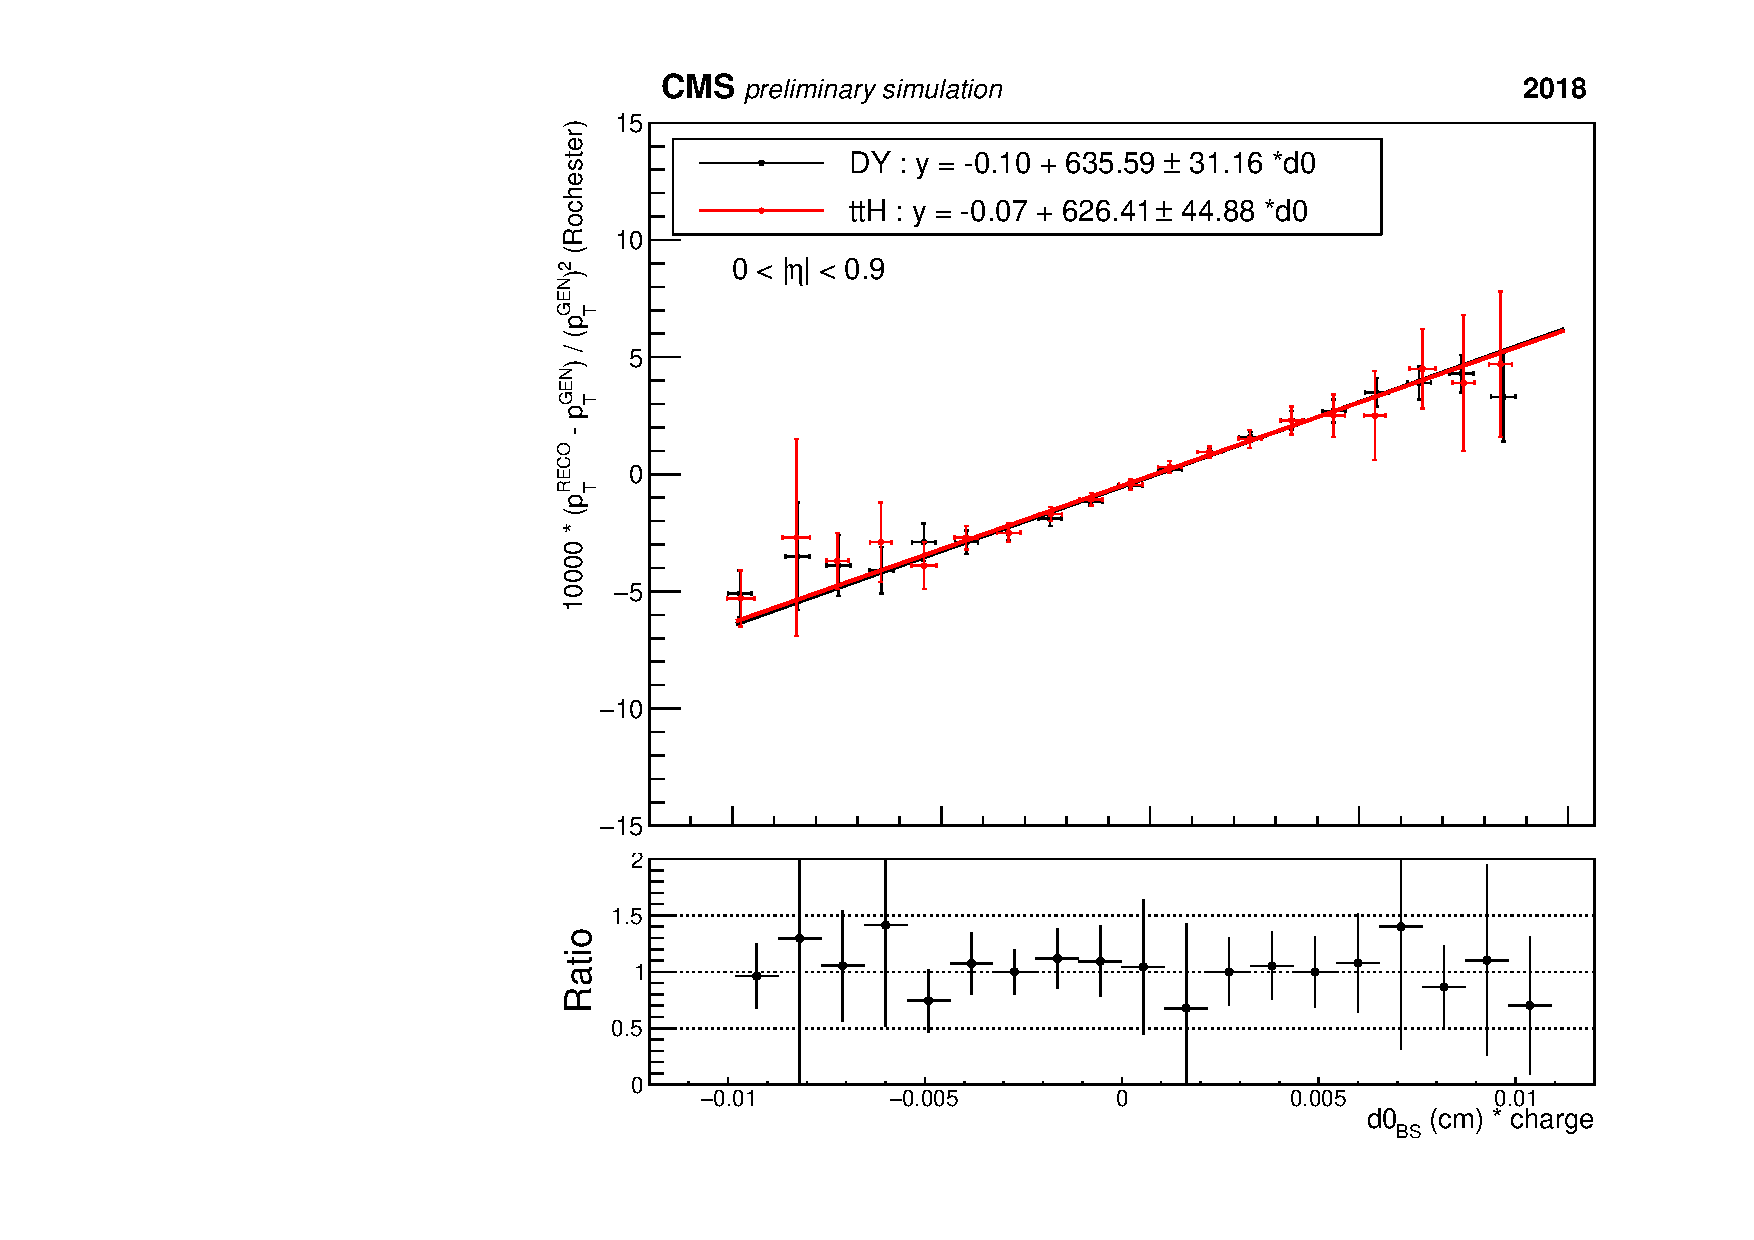
\includegraphics[width=0.32\textwidth]{images_geofit/ttH_eta_0_0p9_2018.pdf}
    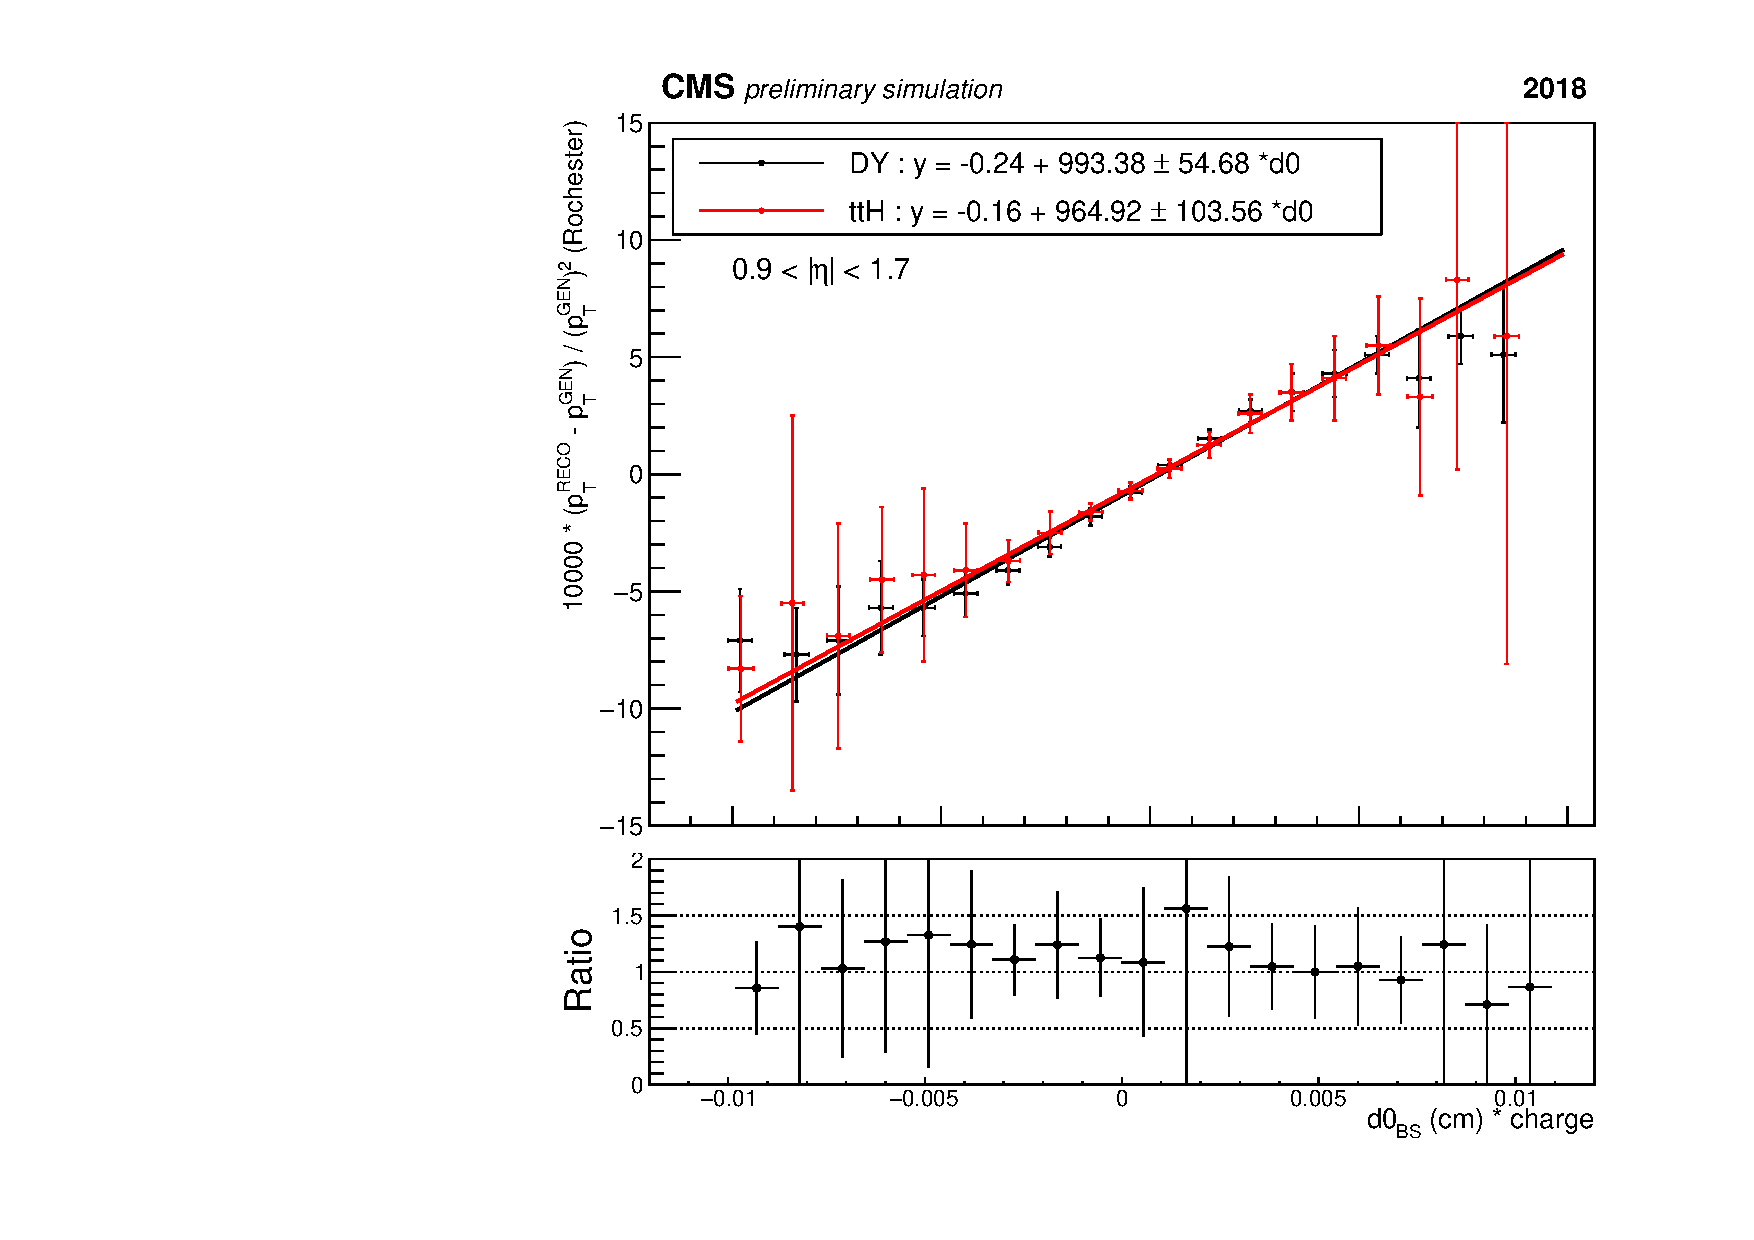
\includegraphics[width=0.32\textwidth]{images_geofit/ttH_eta_0p9_1p7_2018.pdf}
    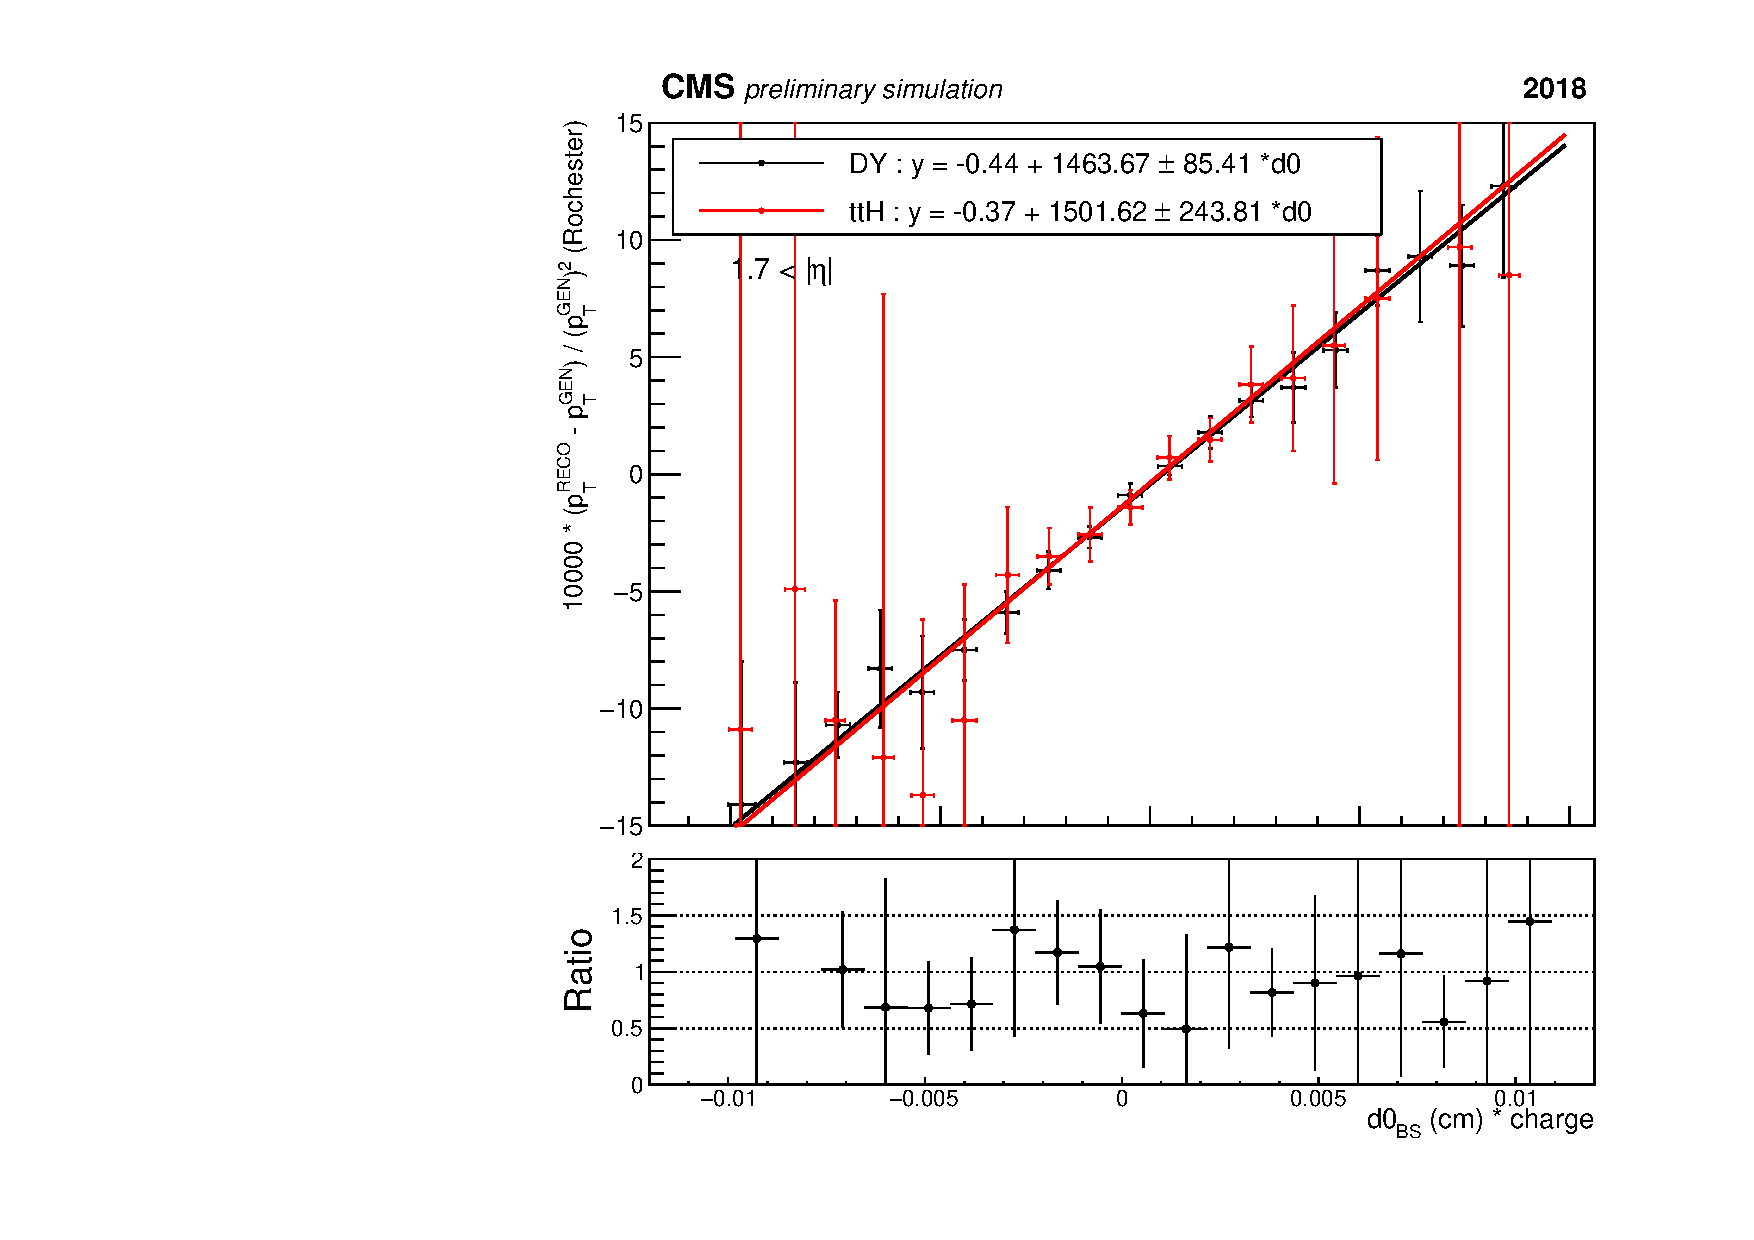
\includegraphics[width=0.32\textwidth]{images_geofit/ttH_eta_1p7_inf_2018.pdf}
    \caption{Plots comparing \dptoverptsquare vs \dzeroBS distributions in each $|\eta|$ region derived from Z+jets MC and ttH MC in 2018. The ratio plot show the ratio between the black data points (Z+jets MC) and the red data points (ttH MC).}
    \label{fig:ttH_d0_2018}
\end{figure}

Finally, Figures~\ref{fig:pt_comp_data_MC_leading} and ~\ref{fig:pt_comp_data_MC_subleading} show comparison of \pt distributions between data and MC for leading and subleading muons, before and after \textit{GeoFit Corrections}. We can see that \textit{GeoFit Corrections} do not change the agreement between \pt distributions in data and MC.

\begin{figure}[h!]
    \centering
    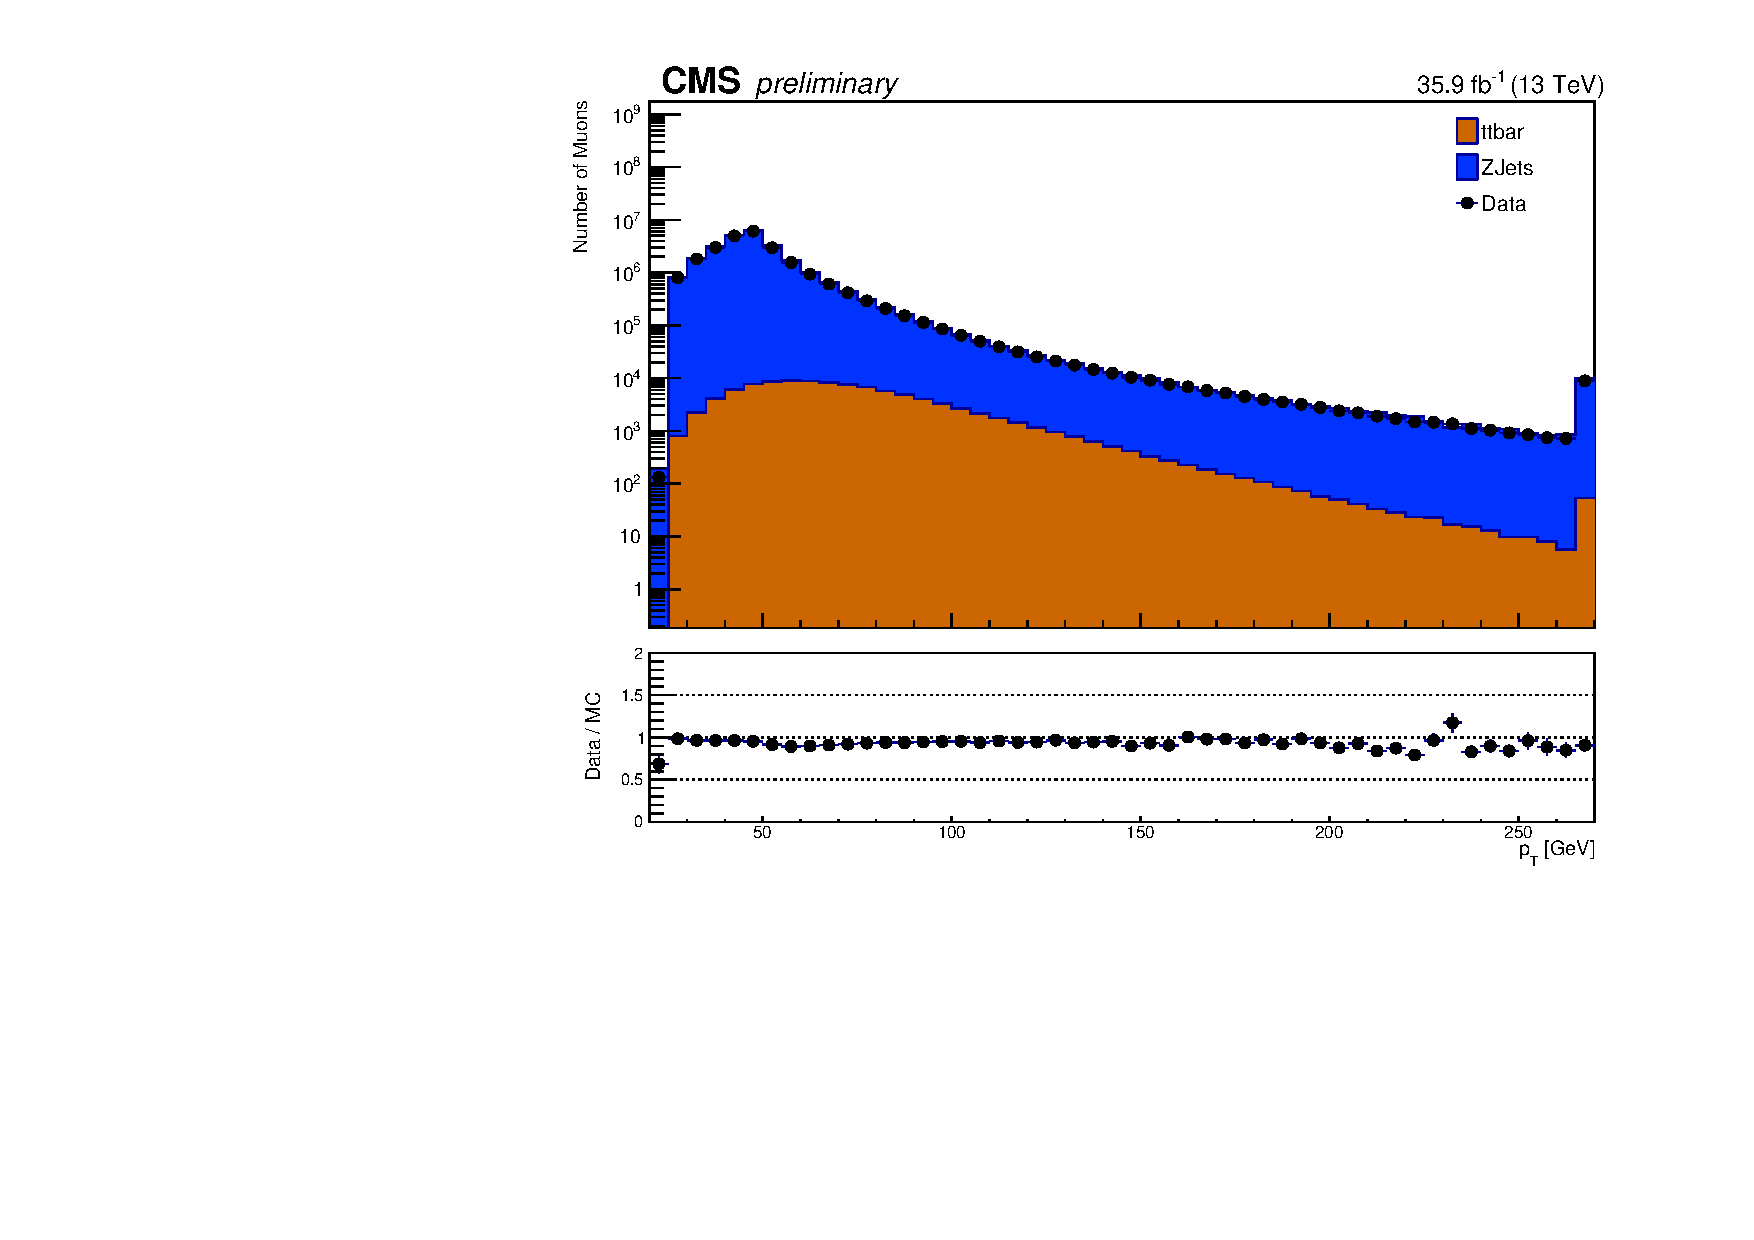
\includegraphics[width=0.49\textwidth]{images_geofit/pt_comp_data_MC_leading_before.pdf}
    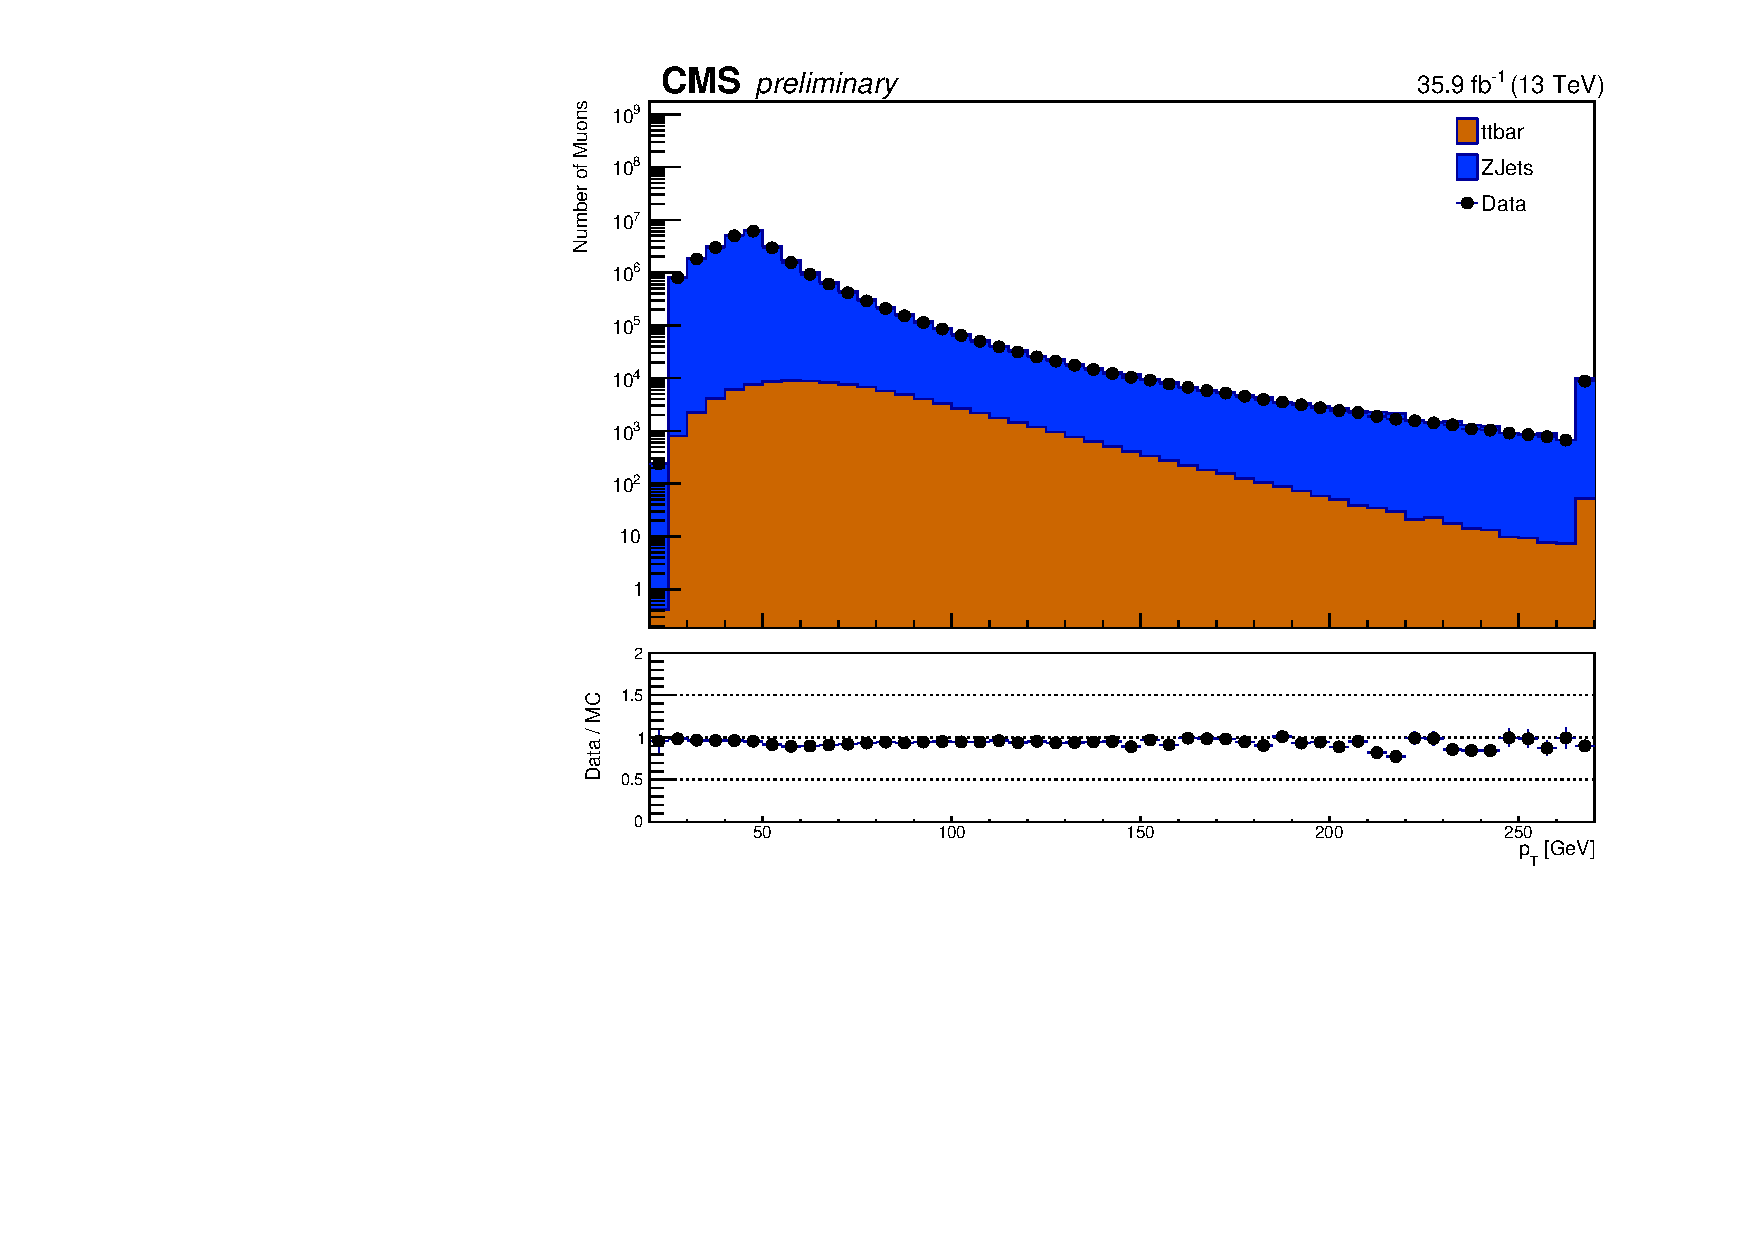
\includegraphics[width=0.49\textwidth]{images_geofit/pt_comp_data_MC_leading_after.pdf}
    \caption{Plots showing the comparison of leading muon \pt between data and MC before (left) and after (right) \textit{GeoFit Corrections}.}
    \label{fig:pt_comp_data_MC_leading}
\end{figure}

\begin{figure}[h!]
    \centering
    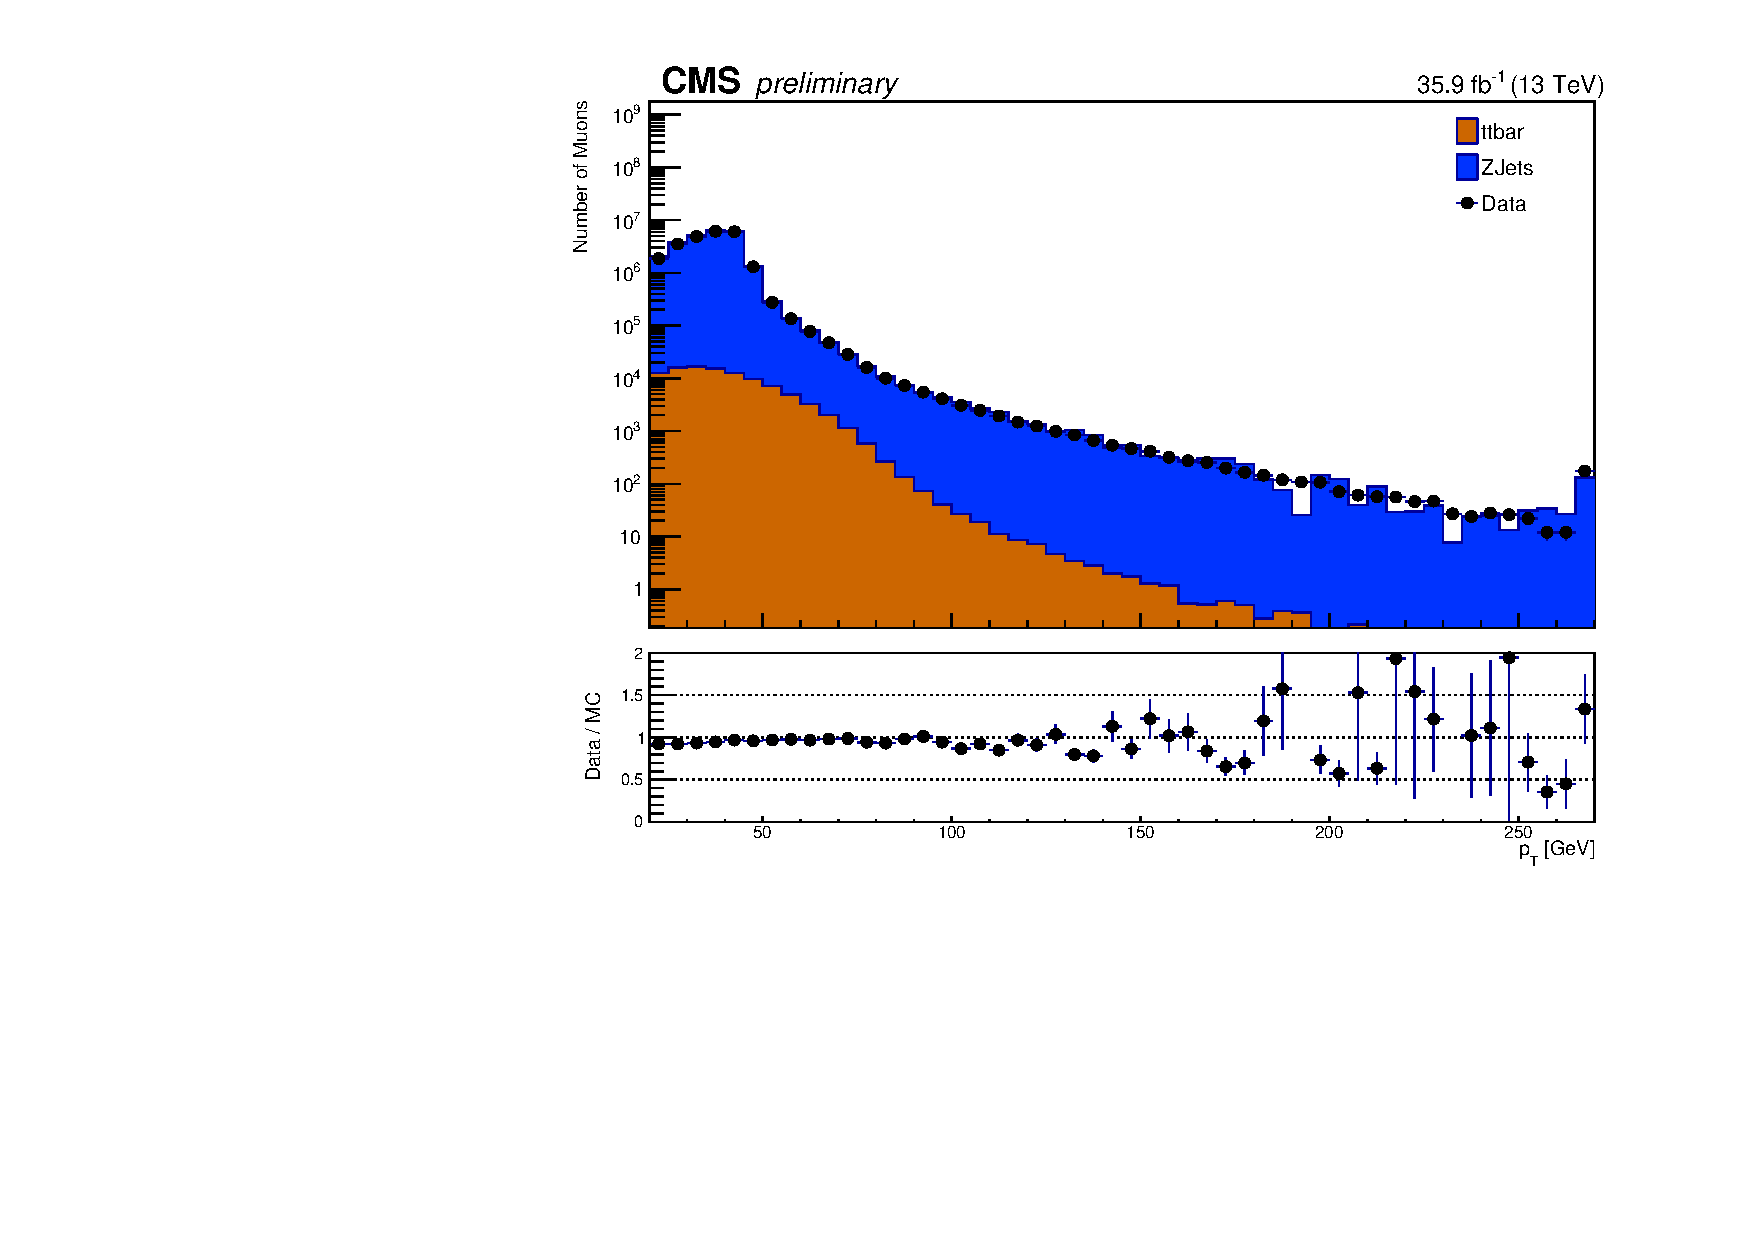
\includegraphics[width=0.49\textwidth]{images_geofit/pt_comp_data_MC_subleading_before.pdf}
    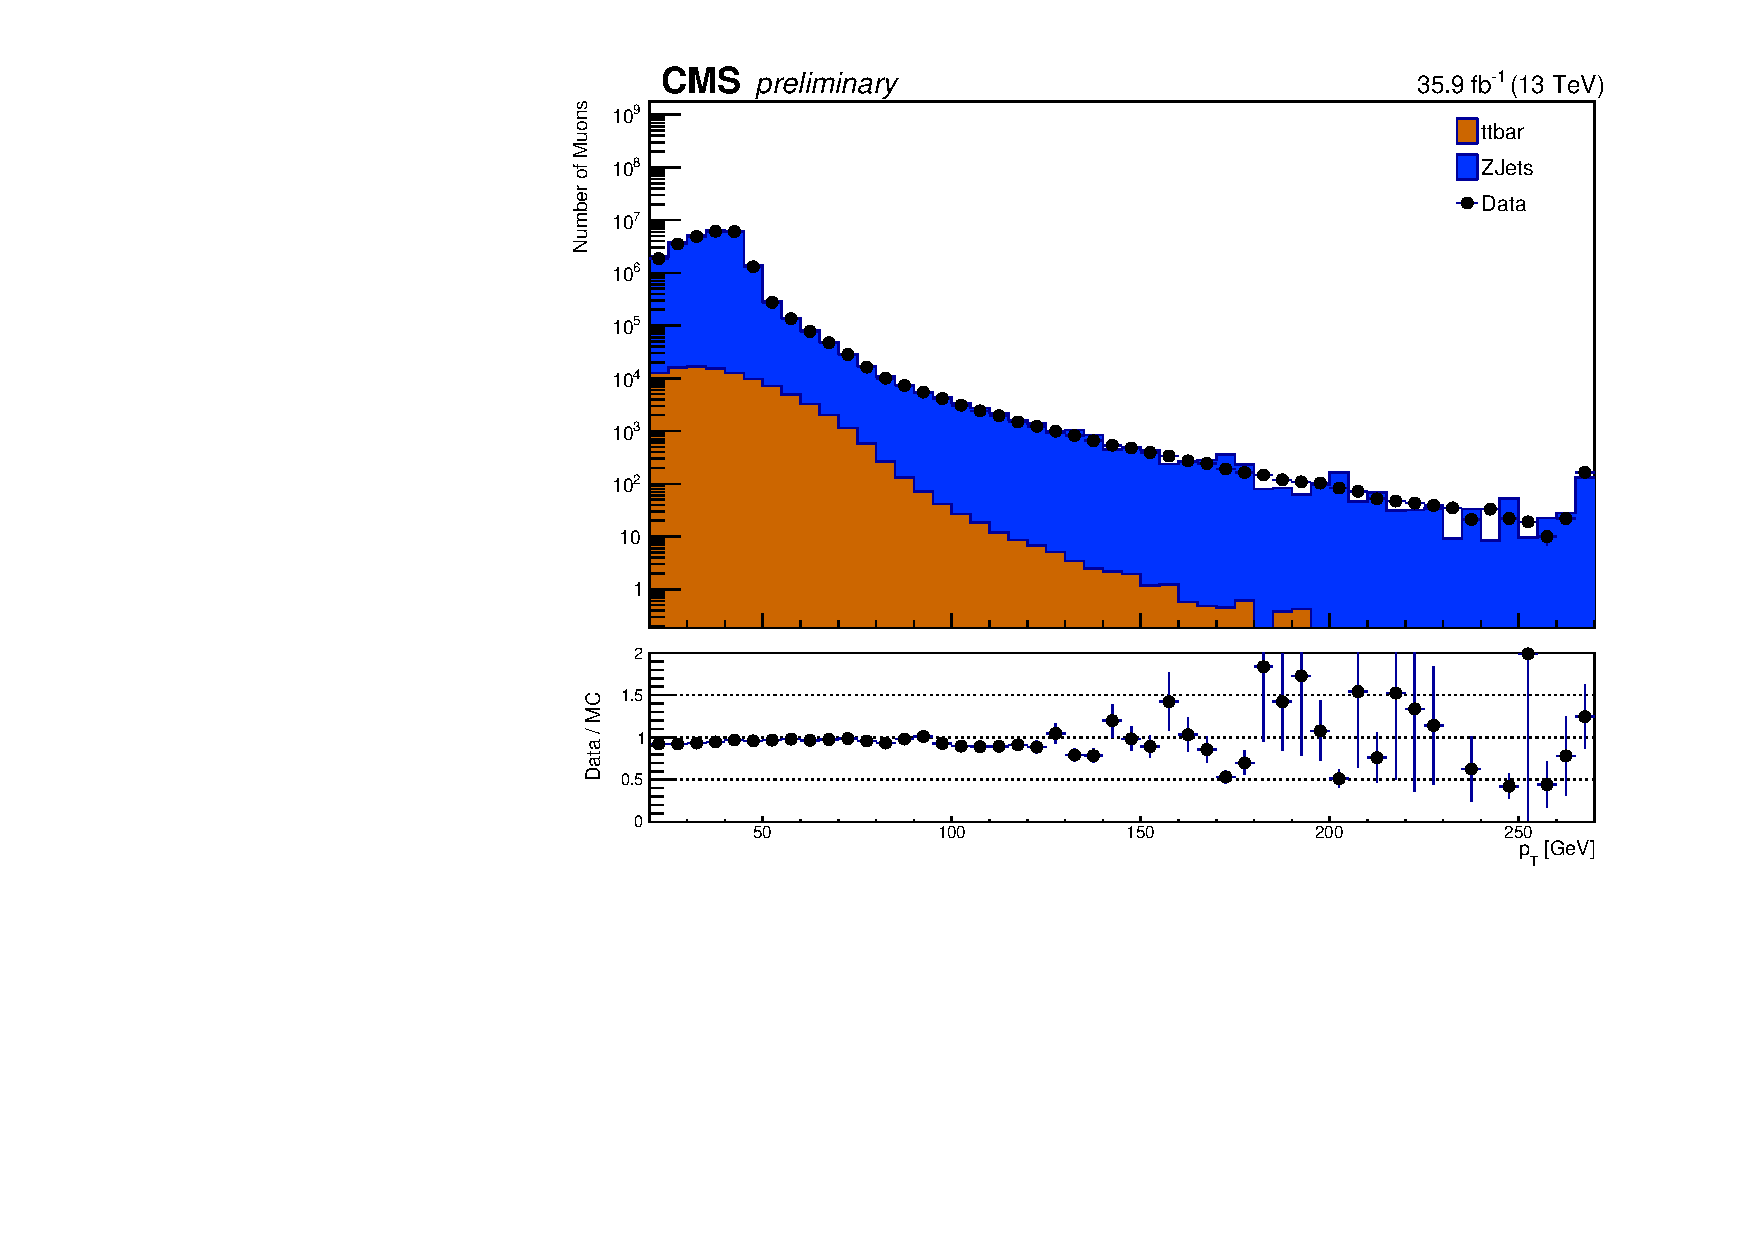
\includegraphics[width=0.49\textwidth]{images_geofit/pt_comp_data_MC_subleading_after.pdf}
    \caption{Plots showing the comparison of subleading muon \pt between data and MC before (left) and after (right) \textit{GeoFit Corrections}.}
    \label{fig:pt_comp_data_MC_subleading}
\end{figure}

% Finally, as a consistency check, Figures~\ref{fig:dpt_tail_core_2016,fig:dpt_tail_core_2017,fig:dpt_tail_core_2018} show \pt resolution distributions of muons, derived from Z+jets MC, in tails and the bulk of \dzeroBS distributions before and after \textit{GeoFit Corrections}. We can see that the muon \pt resolution plots for muons at the tails of \dzeroBS distributions are shifted to lower or higher values depending on the sign of \dzeroBS. This effect is mostly corrected after applying \textit{GeoFit Corrections} which results in an improved muon \pt resolution. 

% \begin{figure}[h!]
%     \centering
%     % \includegraphics[width=1\textwidth]{images_categories/signal_composition_v4_2017.pdf}
%     % \includegraphics[width=1\textwidth]{images_doublemuon/signal_composition_v4_2017_DoubleMuon.pdf}
%     \caption{
    
%     }
%     \label{fig:dpt_tail_core_2016}
% \end{figure}

% \begin{figure}[h!]
%     \centering
%     % \includegraphics[width=1\textwidth]{images_categories/signal_composition_v4_2017.pdf}
%     % \includegraphics[width=1\textwidth]{images_doublemuon/signal_composition_v4_2017_DoubleMuon.pdf}
%     \caption{
    
%     }
%     \label{fig:dpt_tail_core_2017}
% \end{figure}

% \begin{figure}[h!]
%     \centering
%     % \includegraphics[width=1\textwidth]{images_categories/signal_composition_v4_2017.pdf}
%     % \includegraphics[width=1\textwidth]{images_doublemuon/signal_composition_v4_2017_DoubleMuon.pdf}
%     \caption{
    
%     }
%     \label{fig:dpt_tail_core_2018}
% \end{figure}

After checking all the dependencies we can determine that the \textit{GeoFit Corrections} only depend strongly on muon $\eta$ and the era of the MC samples. The latter dependency can be explained by different detector conditions and reconstructed algorithms used in different eras. Due to improvements in inner tracker and BS calculation algorithms we expect the performance of \textit{GeoFit Corrections} to improve from 2016 to 2018. 

Figures~\ref{fig:dimu_mass_DY_MC, fig:dimu_mass_DY_data, fig:dimu_mass_ggH, fig:dimu_mass_VBF, fig:dimu_mass_VH, fig:dimu_mass_ttH} show the comparison of dimuon mass peaks for Z+jets, ggH, VBF, VH and ttH MC and Z+jets data before and after the \textit{GeoFit Corrections}. The resulting improvements for MC samples are compatible with our expectations with the performance improving from 2016 to 2018. The improvements in Z+jets data are also consistent with Z+jets MC with data performing slightly better overall. 

\begin{figure}[h!]
    \centering
    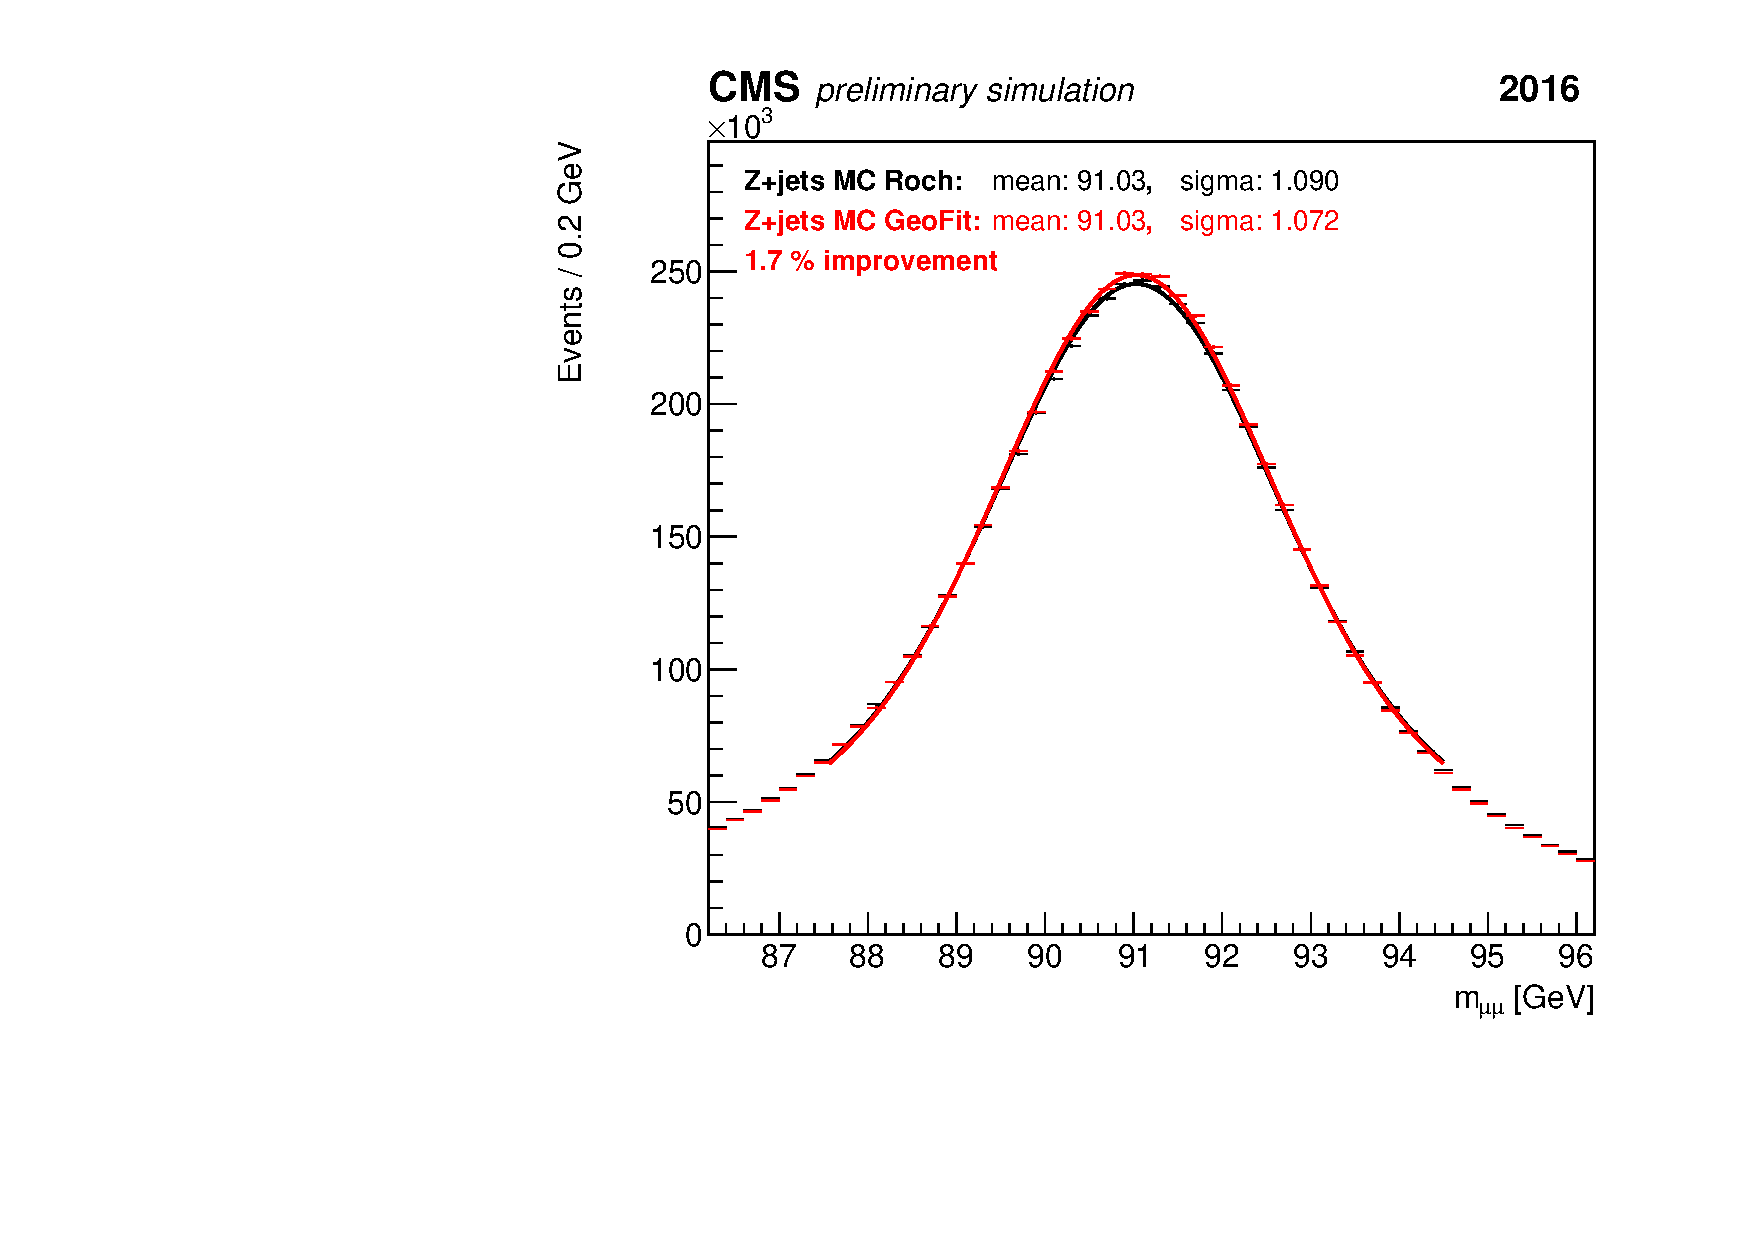
\includegraphics[width=0.32\textwidth]{images_geofit/DY_MC_mass_geofit_2016.pdf}
    \includegraphics[width=0.32\textwidth]{images_geofit/DY_MC_mass_geofit_2017.pdf}
    \includegraphics[width=0.32\textwidth]{images_geofit/DY_MC_mass_geofit_2018.pdf}
    \caption{Dimuon mass peak around 91 \gev for Z+jets MC samples in 2016 (left), 2017 (center) and 2018 (right) fitted by using a Voigtian+exponential function.}
    \label{fig:dimu_mass_DY_MC}
\end{figure}

\begin{figure}[h!]
    \centering
    \includegraphics[width=0.32\textwidth]{images_geofit/DY_data_mass_geofit_2016.pdf}
    \includegraphics[width=0.32\textwidth]{images_geofit/DY_data_mass_geofit_2017.pdf}
    \includegraphics[width=0.32\textwidth]{images_geofit/DY_data_mass_geofit_2018.pdf}
    \caption{Dimuon mass peak around 91 \gev for Z+jets data samples in 2016 (left), 2017 (center) and 2018 (right) fitted by using a Voigtian+exponential function.}
    \label{fig:dimu_mass_DY_data}
\end{figure}

\begin{figure}[h!]
    \centering
    \includegraphics[width=0.32\textwidth]{images_geofit/ggH_mass_geofit_2016.pdf}
    \includegraphics[width=0.32\textwidth]{images_geofit/ggH_mass_geofit_2017.pdf}
    \includegraphics[width=0.32\textwidth]{images_geofit/ggH_mass_geofit_2018.pdf}
    \caption{Dimuon mass peak around 125 \gev for ggH signal MC samples in 2016 (left), 2017 (center) and 2018 (right) fitted by using a double-sided crystal ball function.}
    \label{fig:dimu_mass_ggH}
\end{figure}

\begin{figure}[h!]
    \centering
    \includegraphics[width=0.32\textwidth]{images_geofit/VBF_mass_geofit_2016.pdf}
    \includegraphics[width=0.32\textwidth]{images_geofit/VBF_mass_geofit_2017.pdf}
    \includegraphics[width=0.32\textwidth]{images_geofit/VBF_mass_geofit_2018.pdf}
    \caption{Dimuon mass peak around 125 \gev for VBF signal MC samples in 2016 (left), 2017 (center) and 2018 (right) fitted by using a double-sided crystal ball function.}
    \label{fig:dimu_mass_VBF}
\end{figure}

\begin{figure}[h!]
    \centering
    \subfigure[]{\label{fig:dimu_mass_VH_ZH_2016}\includegraphics[width=0.49\textwidth]{images_geofit/ZH_mass_geofit_2016.pdf}}
    \subfigure[]{\label{fig:dimu_mass_VH_ZH_2018}\includegraphics[width=0.49\textwidth]{images_geofit/ZH_mass_geofit_2018.pdf}}
    \hfill
    \subfigure[]{\label{fig:dimu_mass_VH_WH_neg_2016}\includegraphics[width=0.49\textwidth]{images_geofit/WH_neg_mass_geofit_2016.pdf}}
    \subfigure[]{\label{fig:dimu_mass_VH_WH_neg_2018}\includegraphics[width=0.49\textwidth]{images_geofit/WH_neg_mass_geofit_2018.pdf}}
    \hfill
    \subfigure[]{\label{fig:dimu_mass_VH_WH_pos_2016}\includegraphics[width=0.49\textwidth]{images_geofit/WH_pos_mass_geofit_2016.pdf}}
    \subfigure[]{\label{fig:dimu_mass_VH_WH_pos_2018}\includegraphics[width=0.49\textwidth]{images_geofit/WH_pos_mass_geofit_2018.pdf}}
    \caption{Dimuon mass peak around 125 \gev for VH signal MC samples for ZH in 2016 (top left), ZH in 2018 (top right), WH negative in 2016 (middle left), WH negative in 2018 (middle right), WH positive in 2016 (bottom left), WH positive in 2018 (bottom right) fitted by using a double-sided crystal ball function.}
    \label{fig:dimu_mass_VH}
\end{figure}

\begin{figure}[h!]
    \centering
    \includegraphics[width=0.32\textwidth]{images_geofit/ttH_mass_geofit_2016.pdf}
    \includegraphics[width=0.32\textwidth]{images_geofit/ttH_mass_geofit_2017.pdf}
    \includegraphics[width=0.32\textwidth]{images_geofit/ttH_mass_geofit_2018.pdf}
    \caption{Dimuon mass peak around 125 \gev for ttH signal MC samples in 2016 (left), 2017 (center) and 2018 (right) fitted by using a double-sided crystal ball function.}
    \label{fig:dimu_mass_ttH}
\end{figure}

One interesting aspect of \textit{GeoFit Corrections} is that the performance of these corrections improve with increasing average \pt of muons. This is consistent with the geometric nature of these corrections since this effect scales with $\pt^2$. This results in a better performance for \textit{GeoFit Corrections} in ggH, VBF, VH, and ttH signal samples compared to Z+jets samples.

The uncertainties on \textit{GeoFit Corrections} are mostly due to the derivation of the constant of proportionality. The fitting uncertainties are usually on the order of $10\%$. These uncertainties are assumed to be covered by signal shape fitting uncertainties, and are not propagated to the final corrected muon \pt.









